%% ----------------------------------------
%%
%% NYU PhD thesis template.
%% Created by José Koiller 2007--2008.
%% Modified by Siddharth Krishna, 2019.
%%
%% ----------------------------------------


%% Use the first of the following lines during production to
%% easily spot "overfull boxes" in the output. Use the second
%% line for the final version.
%\documentclass[12pt,draft,letterpaper]{report}
\documentclass[12pt,oneside,letterpaper]{report}


% ----------------------------------------
% Macro to switch between draft version and final version
% ----------------------------------------

% Use or comment this to enable/disable draft version
% \def\draftversion{}
\newcommand{\draftfinal}[2]{\ifdefined\draftversion#1\else#2\fi}
\newcommand{\draftonly}[1]{\draftfinal{#1}{}}
\newcommand{\finalonly}[1]{\draftfinal{}{#1}}


% ----------------------------------------
% Thesis metadata
% ----------------------------------------

%% Replace the title, name, advisor name, graduation date and dedication below
%% with your own. Graduation months must be January, May or September.
\newcommand{\thesistitle}{TBD}
\newcommand{\thesisauthor}{Peixian Wang}
\newcommand{\thesisadvisor}{Professor Ismail Alatas}
\newcommand{\thesisdept}{Hagop Kevorkian Center for Near Eastern Studies, GSAS}
\newcommand{\gradmonth}{May}
\newcommand{\gradyear}{2023}
%% If you do not want a dedication, scroll down and comment out
%% the appropriate lines in this file.
\newcommand{\thesisdedication}{To my dog Weierstra\ss, with affection.}


% ----------------------------------------
% Layout and formatting
% ----------------------------------------

% Uncomment to get a big black box to spot "overfull hboxes"
% \setlength{\overfullrule}{5pt}


%% Page layout (customized to letter paper and NYU requirements):
\RequirePackage[margin=1in, includefoot, letterpaper]{geometry}


%% Color definitions:
\RequirePackage[prologue]{xcolor}
\definecolor[named]{ThesisBlue}{cmyk}{1,0.1,0,0.1}
\definecolor[named]{ThesisYellow}{cmyk}{0,0.16,1,0}
\definecolor[named]{ThesisOrange}{cmyk}{0,0.42,1,0.01}
\definecolor[named]{ThesisRed}{cmyk}{0,0.90,0.86,0}
\definecolor[named]{ThesisLightBlue}{cmyk}{0.49,0.01,0,0}
\definecolor[named]{ThesisGreen}{cmyk}{0.20,0,1,0.19}
\definecolor[named]{ThesisPurple}{cmyk}{0.55,1,0,0.15}
\definecolor[named]{ThesisDarkBlue}{cmyk}{1,0.58,0,0.21}

% School color found from university's graphic identity site:
% http://www.nyu.edu/employees/resources-and-services/media-and-communications/styleguide.html
\definecolor{SchoolColor}{rgb}{0.3412, 0.0235, 0.5490} % purple
\definecolor{chaptergrey}{rgb}{0.2600, 0.0200, 0.4600} % dialed back a little
\definecolor{midgrey}{rgb}{0.4, 0.4, 0.4}

\usepackage{hyperref}
\hypersetup{colorlinks,
  linkcolor=ThesisDarkBlue,
  citecolor=ThesisPurple,
  urlcolor=ThesisDarkBlue,
  filecolor=ThesisDarkBlue}


%% Captions of Figures, tables
\RequirePackage[labelfont={bf,sf,small,singlespacing},
                textfont={sf,small,singlespacing},
                % justification={justified,RaggedRight},
                % singlelinecheck=false,
                margin=0pt,
                figurewithin=chapter,
                tablewithin=chapter]{caption}

%% Chapter headings, captions
\usepackage{fix-cm}
\RequirePackage[raggedright,sc]{titlesec}
\definecolor{gray75}{gray}{0.75}
\newcommand{\hsp}{\hspace{20pt}}

\titleformat{\chapter}[hang]
{\Huge\sc}
{\textcolor{SchoolColor}{\thechapter}\hsp\textcolor{gray75}{|}\hsp}
{0pt}{\Huge\sc\raggedright}
% [\textcolor{gray75}{|}\hsp\textcolor{SchoolColor}{\thechapter}]


%% The following makes chapters and sections, but not subsections,
%% appear in the TOC (table of contents). Increase to 2 or 3 to
%% make subsections or subsubsections appear, respectively. It seems
%% to be usual to use the "1" setting, however.
\setcounter{tocdepth}{2}

%% Sectional units up to subsubsections are numbered. To number
%% subsections, but not subsubsections, decrease this counter to 2.
\setcounter{secnumdepth}{3}

%% Use the following commands, if desired, during production.
%% Comment them out for final version.
%\usepackage{layout} % defines the \layout command, see below
%\setlength{\hoffset}{-.75in} % creates a large right margin for notes and \showlabels

%% Controls spacing between lines (\doublespacing, \onehalfspacing, etc.):
\usepackage{setspace}

%% Use the line below for official NYU version, which requires
%% double line spacing. For all other uses, this is unnecessary,
%% so the line can be commented out.
\finalonly{
  \doublespacing % requires package setspace, invoked above
}


% ----------------------------------------
% Comments and TODOs:
% ----------------------------------------

% Uncomment this to remove all comments
\newcommand{\nocomments}{}

% Uncomment this to remove all TODOs
\newcommand{\notodos}{}

% Comments and TODOs
\newcommand{\fcomment}[2]{\ifdefined\nocomments{}\else\footnote{\textcolor{red}{#1:} #2}\fi}
\newcommand{\todo}[1]{\ifdefined\notodos{}\else\textcolor{red}{TODO\ifstrempty{#1}{}{: #1}}\fi}
\newcommand{\ftodo}[1]{\ifdefined\notodos{}\else\fcomment{TODO}{#1}\fi}


% Author comments:
\newcommand{\aen}[1]{\fcomment{Emmy}{#1}}


% ----------------------------------------
% User-specific packages and macros
% ----------------------------------------

%% This inputs your auxiliary file with \usepackage's and \newcommand's:
%% It is assumed that that file is called "defs.tex".
% ----------------------------------------
% Packages
% ----------------------------------------

% 
% Place here your \usepackage's. Some recommended packages are already included.
%

% Graphics:
\usepackage[final]{graphicx}
%\usepackage{graphicx} % use this line instead of the above to suppress graphics in draft copies
%\usepackage{graphpap} % \defines the \graphpaper command

% Uncomment this to indent first line of each section:
% \usepackage{indentfirst}
\graphicspath{ {./images/} }
% Good AMS stuff:
\usepackage{amsthm} % facilities for theorem-like environments
\usepackage[tbtags]{amsmath} % a lot of good stuff!

% Fonts and symbols:
\usepackage{times}
\usepackage{amssymb}
\newcommand\myworries[1]{\textcolor{red}{#1}}


% Set the fonts

% For typesetting inference rules
\usepackage{mathpartir}
% \usepackage{pftools}  % A local package
\newcommand{\bmmax}{2}
\usepackage{bm}

% Formatting tools:
%\usepackage{relsize} % relative font size selection, provides commands \textsmalle, \textlarger
%\usepackage{xspace} % gentle spacing in macros, such as \newcommand{\acims}{\textsc{acim}s\xspace}

% Page formatting utility:
%\usepackage{geometry}

\usepackage{booktabs}   %% For formal tables:
                        %% http://ctan.org/pkg/booktabs
\usepackage[labelformat=simple]{subcaption} %% For complex figures with subfigures/subcaptions
                        %% http://ctan.org/pkg/subcaption
% Options to subcaption are to label and refer to subfigures as Fig 1(a) etc.
\renewcommand\thesubfigure{(\alph{subfigure})}

\usepackage[T1]{fontenc} % needed for scaling fancy fonts (?)
\usepackage[utf8]{} % not sure this is needed
\usepackage{fontspec}

\usepackage{amssymb}
%\usepackage[table]{xcolor}

\usepackage{float}
% For code
\usepackage[final]{listings}
\lstset{mathescape=true}

% For code highlighting
% \usepackage{bold-extra}
% Tikz
\usepackage{tikz}
\usetikzlibrary{matrix,arrows,positioning,calc,fit,backgrounds}

% To control enum item labelling/numbering
\usepackage[shortlabels, inline]{enumitem}
% To give custom item labels and reference them
\makeatletter
\newcommand{\myitem}[1][]{
  \protected@edef\@currentlabel{#1}%
\item[#1]
}
\makeatother

% To stop aligned env swallowing up []s
\usepackage{mathtools}

% To use ifstrempty
\usepackage{etoolbox}

% For math mode tables
\usepackage{array}
% A text column in array
\newcolumntype{L}{>$l<$}

% For \llbracket and \rrbracket
\usepackage{stmaryrd}

% For dashed boxes
\usepackage{dashbox}

% For big separating conjunction
\usepackage{scalerel}

% For mathpar environment
\usepackage{mathpartir}

\usepackage{xspace}
\usepackage{multirow}

% To stop citations overflowing lines
\usepackage{breakcites}

\usepackage{csquotes}


% For citet command
\usepackage{natbib}
\setcitestyle{%
    authoryear,%
    open={[},close={]},citesep={;},%
    aysep={},yysep={,},%
    notesep={, }}
\let\cite\citep


\usepackage{polyglossia}
\setdefaultlanguage{english}
\setotherlanguage{arabic}
\setmainfont{STIX Two}[
  UprightFont={* Math},
  ItalicFont={* Text Italic},
  BoldFont={* Text Bold},
  BoldItalicFont={* Text Bold Italic},
]

\newfontfamily\arabicfont[Script=Arabic,ItalicFont=*,Scale=1.75]{Scheherazade}

%%
%% Place here your \newtheorem's:
%%

% \theoremstyle{plain}
% \newtheorem{theorem}{Theorem}[chapter]
% \newtheorem{conjecture}[theorem]{Conjecture}
% \newtheorem{proposition}[theorem]{Proposition}
% \newtheorem{lemma}[theorem]{Lemma}
% \newtheorem{corollary}[theorem]{Corollary}
% \theoremstyle{definition}
% \newtheorem{example}[theorem]{Example}
% \newtheorem{definition}[theorem]{Definition}
% \theoremstyle{plain}


% ----------------------------------------
% Generic definitions
% ----------------------------------------
% Required packages: listings, tikz

% A footnote without a marker
\newcommand\blfootnote[1]{%
  \begingroup
  \renewcommand\thefootnote{}\footnote{#1}%
  \addtocounter{footnote}{-1}%
  \endgroup
}

\renewcommand{\le}{\leqslant}
\renewcommand{\ge}{\geqslant}
% \renewcommand{\emptyset}{\ensuremath{\varnothing}}
% \newcommand{\ds}{\displaystyle}


%% Caligraphic
\newcommand{\Aa}{{\mathcal{A}}}
\newcommand{\Bb}{{\mathcal{B}}}
\newcommand{\Cc}{{\mathcal{C}}}
\newcommand{\Dd}{{\mathcal{D}}}
\newcommand{\Ee}{{\mathcal{E}}}
\newcommand{\Ff}{{\mathcal{F}}}
\newcommand{\Gg}{{\mathcal{G}}}
\newcommand{\Hh}{{\mathcal{H}}}
\newcommand{\Ii}{{\mathcal{I}}}
\newcommand{\Jj}{{\mathcal{J}}}
\newcommand{\Kk}{{\mathcal{K}}}
\newcommand{\Ll}{{\mathcal{L}}}
\newcommand{\Mm}{{\mathcal{M}}}
\newcommand{\Nn}{{\mathcal{N}}}
\newcommand{\Oo}{{\mathcal{O}}}
\newcommand{\Pp}{{\mathcal{P}}}
\newcommand{\Qq}{{\mathcal{Q}}}
\newcommand{\Rr}{{\mathcal{R}}}
\newcommand{\Ss}{{\mathcal{S}}}
\newcommand{\Tt}{{\mathcal{T}}}
\newcommand{\Uu}{{\mathcal{U}}}
\newcommand{\Vv}{{\mathcal{V}}}
\newcommand{\Ww}{{\mathcal{W}}}
\newcommand{\Yy}{{\mathcal{Y}}}
\newcommand{\Zz}{{\mathcal{Z}}}

% Wrappers: Parens, brackets, etc
% \newcommand{\op}[1]{\operatorname{#1}}
\newcommand{\paren} [1] {\ensuremath{ \left( {#1} \right) }}
\newcommand{\bigparen} [1] {\ensuremath{ \Big( {#1} \Big) }}
% \newcommand{\bracket}[1]{\left[#1\right]}
\newcommand{\tuple}[1]{\ensuremath{\langle #1 \rangle}}
\newcommand{\abs}[1]{\ensuremath{\lvert #1 \rvert}}
% \newcommand{\set}[1]{\ensuremath{\left\{#1\right\}}}
\newcommand{\setcomp}[2]{\ensuremath{\left\{#1\;\middle|\;#2\right\}}}

% References
\newcommand{\refCh}[1]{Chapter~\ref{#1}}
\newcommand{\refSc}[1]{Section~\ref{#1}}
% \newcommand{\refSc}[1]{\S\ref{#1}}
\newcommand{\refFig}[1]{Figure~\ref{#1}}
\newcommand{\refDef}[1]{Definition~\ref{#1}}
\newcommand{\refLem}[1]{Lemma~\ref{#1}}
\newcommand{\refThm}[1]{Theorem~\ref{#1}}
\newcommand{\refAlg}[1]{Algorithm~\ref{#1}}
\newcommand{\refEx}[1]{Example~\ref{#1}}
\newcommand{\refCor}[1]{Corollary~\ref{#1}}
\newcommand{\refTab}[1]{Table~\ref{#1}}
\newcommand{\refEq}[1]{\ensuremath{(\ref{#1})}}
\newcommand{\refRule}[1]{(\ref{#1})}
\newcommand{\refApp}[1]{Appendix~\ref{#1}}

\newcommand{\tool}[1]{\textsf{#1}}
\newcommand{\code}[1]{\textnormal{\small\texttt{#1}}}
% \newcommand{\code}[1]{\text{\lstinline{#1}}}

% TODO have macros for \forall and \exists

\newcommand{\tick}{\ensuremath{\checkmark}}
\newcommand{\cross}{\text{\sffamily X}}

\interfootnotelinepenalty=10000
% ----------------------------------------
% Paper specific macros & commands
% ----------------------------------------


% Put your definitions here
% \newcommand{\arahamza}{{\fontspec{Symbola}\char"02BE}}
% \newcommand{\arah}{{\fontspec{Symbola}\char"1E25}}
% \newcommand{\aras}{{\fontspec{Symbola}\char"1E63}}
% \newcommand{\arad}{{\fontspec{Symbola}\char"1E0D}}
% \newcommand{\arat}{{\fontspec{Symbola}\char"1E6D}}
% \newcommand{\arath}{{\fontspec{Symbola}\char"1E93}}
% \newcommand{\araayn}{{\fontspec{Symbola}\char"02BF}}
% \newcommand{\araalif}{{\fontspec{Symbola}\char"1D44E\char"0304}}
% \newcommand{\arawaw}{{\fontspec{Symbola}\char"1D462\char"0304}}
% \newcommand{\araei}{{\fontspec{Symbola}\char"1D73E\char"0304}}

%%% Local Variables:
%%% mode: latex
%%% TeX-master: "thesis"
%%% End:




% ----------------------------------------
% Document header
% ----------------------------------------

%% Cross-referencing utilities. Use one or the other--whichever you prefer--
%% but comment out both lines for final version.
%\usepackage{showlabels}
%\usepackage{showkeys}

\begin{document}
%% Produces a test "layout" page, for "debugging" purposes only.
%% Comment out for final version.
%\layout % requires package layout (see above, on this same file)


%%%%%% Title page %%%%%%%%%%%
%% Sets page numbering to "roman style" i, ii, iii, iv, etc:
\pagenumbering{roman}
%
%% No numbering in the title page:
\thispagestyle{empty}
%
\vspace*{25pt}
\begin{center}
  {\Large
    \begin{doublespace}
      {\textcolor{SchoolColor}{\textsc{\thesistitle}}}
    \end{doublespace}
  }
  \vspace{.7in}

  by
  \vspace{.7in}

  \thesisauthor
  \vfill

  \begin{doublespace}
    \textsc{
    % A dissertation submitted in partial fulfillment\\
    % of the requirements for the degree of\\
    % Doctor of Philosophy\\
    \thesisdept\\
    New York University\\
    \gradmonth, \gradyear}
  \end{doublespace}
\end{center}
\vfill

\noindent\makebox[\textwidth]{\hfill\makebox[2.5in]{\hrulefill}}\\
\makebox[\textwidth]{\hfill\makebox[2.5in]{\hfill\thesisadvisor}}

\newpage


%%%%%%%%%%%%%% Dedication %%%%%%%%%%%%%%%%%
%% Comment out the following lines if you do not want to dedicate
%% this to anyone...
% \cleardoublepage
% \phantomsection
% \addcontentsline{toc}{chapter}{Dedication}
% \vspace*{\fill}
% \begin{center}
%   \thesisdedication
% \end{center}
% \vfill
% \newpage


%%%%%%%%%%%%%% Acknowledgements %%%%%%%%%%%%
%% Comment out the following lines if you do not want to acknowledge
%% anyone's help...
\chapter*{Acknowledgements}
\addcontentsline{toc}{chapter}{Acknowledgments}
% This research owes a deep debt to the various people in Iraq, locals and foreigners alike. I owe a debt of gratitude to my advisor, Professor Ismail Alatas, and my thesis reader, Professor Sara Pursely, for their support throughout this entire project.
A thousand thanks to Mélisande Genat for blazing a path for research in Iraq, this research would have been impossible without her. I have to commend Yasmine Mosimann, Haley Bobseine, and Sam Sweeney for their patience and willingness to hear out and challenge my ideas. A special thanks to Abu Shams and Doctor Nofour Abbas, who both helped me greatly in grasping the rich context of Karbala. To my many interviewees that I badgered with questions, many of whom sadly must go unnamed in this thesis, I am forever indebted to the all of you. A great thanks to Arran Walshe and Professor Alix Phillipon for their help throughout the revising process.

Last, but certainly not least, I must thank everyone at the Shrine of Imam Hussein, especially the janitors: Ali, Hussein, and Kassem. Your generosity in opening the rooftop for me every evening to sleep preserved my sanity in those 40 degree summer nights. 

\newpage


%%%% Abstract %%%%%%%%%%%%%%%%%%
\chapter*{Abstract}
\addcontentsline{toc}{chapter}{Abstract}

This study offers a novel exploration of the vital role of religious rituals among Karbala's devout populace, emphasizing the nuanced tensions between the laity and the clerical hierarchy. It scrutinizes various religious entities and ritual participants, including liturgy chanters, known as \emph{radūd}, the Iraqi militias called Hashd al-Shaabi, and local neighborhood assemblies, referred to as \emph{mūkib}. Drawing on unique ethnographic data collected in Karbala, this research reveals that lay Karbalaeis are not mere bystanders in their faith. They actively engage in an intricate contestation of the public sphere and significantly influence the evolution of their religious customs. Critically, this study diverges from the prevalent Najaf-centric research approach in Shi'a religious studies, where the focus has traditionally been on clerics and their relationships with the state or followers. It underscores the substantial role that grassroots actors in Karbala play in molding the religious terrain, thereby presenting a more comprehensive view of Iraq's religious environment that extends beyond Najaf's boundaries.

\newpage


%%%% Table of Contents %%%%%%%%%%%%
\tableofcontents


%%%%% Body of thesis starts %%%%%%%%%%%%
\pagenumbering{arabic} % switches page numbering to arabic: 1, 2, 3, etc.


% ----------------------------------------
% Body of Thesis
% ----------------------------------------

\chapter{Introduction}
\label{introduction}

What do religious rituals mean for pious residents of a shrine city? That is the central question I hope to answer in this thesis. Rituals themselves is already a leaky box of abstraction, intersecting with facets of lived experience, historical imperatives, and religious faith, yet rituals are also expected to play a key role in the formation of faith. 

For rituals to work, certain constraints must be placed upon them. They cannot be too loose with symbols and traditions, which risks tearing the ritual apart and losing meaning and followers. Yet too much rigidity poses the same threat of driving away followers, the nightmare of tradition cannot weigh too heavily on the laity. 

This thesis is focused on two main goals: an accurate description of the experience around rituals within and around Karbala, and an attempt to understand how these rituals provide space for new discourse. 

Some of the essential characteristics can be glimpsed from the unique political context of Karbala: a holy Shi'a city in rivalry with the other holy cities of Shi'ism and Islam in general, situated within a country crawling out of invasion and sectarian wars in the past two decades, all less than 20 kilometers from a cradle of civilization. The past presses close in Karbala, pulling its residents from the cacophony of the present and pushing them into becoming the agents they could otherwise never be. 

Having said what this thesis is about, I should also say what it is not about. The thesis is not a complete review of all Shi'a rituals, it is not the comparative nature of rituals across borders that I am interested in, but rather the merging of the holy city context with rituals. I am also unconcerned with the aspects of belonging and self-transformation that occur to pilgrims, the focus is on the institutions and people who make the rituals happen, as well as the residents of Karbala. 

Women are conspicuously absent within this thesis. This is an unfortunate facet of the Karbala context: as a man, nearly all rituals I observed was only men, and the conservative Islamic context prevented me from conducting extensive fieldwork with women. Rather than attempting to shoehorn a token section on the role of women, I hope that there is further study in the future by someone else on the role of women in Shi'a rituals. 

% As Geartz mentions in his seminal work on culture and religion: "the notion that religion tunes human actions to an envisaged cosmic order and projects images of cosmic order onto the plane of human experience is hardly novel. But it is hardly investigated either, so we have very little idea of how, in empirical terms, this particular miracle is accomplished." \cite[90]{geertz_interpretation_1993} While a pile of ethnographic work supports that this miracle is constructed through repeated actions, yet Geertz rejects this as a sufficient explanation, going on to mention that more theoretical works must be constructed. 

% Repetition is another oft studied facet. From Derrida's iteration and play to eternal pilgrims of Shikoku \cite{reader_pilgrims_2021}, pilgrimage, the idea that repetition itself creates space for change is also hardly novel. 

% What is the argument? The argument is that iteration, with language, photography, and iteration, is the key difference between this and seeing it as a pilgrimage. People aren't seen as pilgrims, especially in Karbala, because they're not pilgrims. Yet they still use the same transformative structures. 

\section{Background}
This project originally began as yet-another-study into sectarianism and sectarianian identity formation within Iraq, specifically focused on the Hashd al-Shaabi. However after sustained fieldwork among the Hashd, my interests shifted into the banality of religious entwinement with the Hashd. After the sheen of militia studies had worn off as another bloody sword to swing, I realized that my research among the Hashd offered a gateway into peering into Karbala. 

Another motivating factor was that nearly every work on post-2003 Iraq centered around either poor people or politics. Due to a dearth of journalists and academics within Iraq, NGOs, especially IOM, had stepped in as local experts on the ground. This lead to journalists seeking NGOs as partners and "experts on the ground", creating a situation where NGOs effective became newsmakers, allowing NGOs to drive reporting and use media outlets as self justification. As NGOs primarily focus on poor people or politics, naturally work from Iraq centered on those two topics.

Even among NGOs, Karbala has remained a relatively understudied site. Najaf's close relations with the government, especially following recent law changes that requires Najaf to nominate the minister of religious endowments \cite{hamoudi_engagements_2020} has drawn the majority of focus towards Najaf. As a result, I decided that Karbala would prove to be a fruitful site in order to conduct research, although at the beginning my work still heavily focused on sectarianism and militia demobilization, disarmament, and reintegration. 

%My original background lies in Physics, Computer Science, and Linguistics. Natural language processing systems such as the GPT flavors have gradually taken over modern computer interfaces, with eschewing traditional linguistics studies of grammar morpology and formulic approaches to language. Frederick Jelinek, a researcher into automatic speech recognition, once famously said "Every time I fire a linguist, the performance of the speech recognizer goes up", referencing how sheer quantities of data have repeatedly outperformed brittle theories of language. I approached my work in the same way, in 

\section{Fieldwork}

Fieldwork was conducted in three major phases, two short visits of a month each in Karbala, a longer active fieldwork phase in Karbala, and a third smaller phase in comparative work in Baghdad. The first two phases of fieldwork were conducted in August 2021 and March 2022 respectively. The longer, active fieldwork consisted of fieldwork between May to October of 2022. A final phase of research focused on Baghdad from January to February 2023. 

Preliminary fieldwork largely was focused on building contacts and finding questions related to the fieldwork. In August 2021, my first visit was during Ashura in Karbala, with frequent travels to Najaf. Additional fieldwork was done in the Kurdish north, specifically with Shi'as residing in Duhok. March 2022 focused on Karbala specifically, with more in depth work about organization and institutions of Shi'a pilgrimage. Between May and October, I mostly resided in Karbala, but made frequent trips to other cities in order to do some comparative analysis, specifically the cities of Tel Afar, Samarra, Hilla, and Baghdad. In the two months of January and February of 2023, I decided to focus on fieldwork within Baghdad, since Baghdad's privileged role as the cultural and population center of Iraq has caused it to develop its own specific culture. 

\section{Organization}

This thesis is organized into two main content chapters. The rest of this introduction focuses on a description of Shi'a politics within contemporary Iraq, as well as a brief background of Shi'ism and religious rituals.

The first content chapter focuses on the role of institutions within Karbala, and how the institutions themselves shape rituals. Writing against traditional literature that focuses its role on the pilgrim, specifically with regards to tourism or the spiritual economy of pilgrimage, I attempt to show that the institutions play an active role in using pilgrims to further their own expansion, which also exposes them to change beyond their control. 

The second chapter focuses on a specific institution: the mowkeb. As the mowkeb lies at the heart of Iraqi Shi'a rituals, the second chapter draws out the history of mowkebs within Karbala, the specific sociolinguistic role they play, and how they act as the final piece in the bridge between tribes, politics, and religion. 

\section{Shiism and the Politics of Iraq}
Iraq's Shi'a majority city all hold specific pilgrimages, referred to as \emph{ziyara} (\begin{Arabic}زِيَارَة\end{Arabic}), or visitations. Four of them: Karbala, Najaf, Samarra, and Baghdad hold shrines for one or more of the twelve Imams. The Shrine of Imam Hussain (the third Imam) and the Shrine of Abbas are in Karbala, the Shrine of Imam Ali (the first Imam) lies in Najaf, the al-Askari Shrine in Samarra contains the tombs of Imam al-Hadi (the tenth Imam) and Imam al-Askari (the eleventh Imam), and the Shrine of Imam al-Kathim contains the tombs of Imam al-Kathim (the seventh Imam) and Imam al-Jawad (the nineth Imam). 

Each shrine has a bureaucratic institution called an \emph{attaba} (\begin{Arabic}عتبة\end{Arabic}). Each attaba is responsible for soliciting donations, upkeep of the shrine, media relations, as well as other religious affairs. In Karbala specifically, the shrines of Abbas and Imam Hussein have separate attabas. Each attaba has an independent media affairs office, independent museums, radio stations, archives, and so on. The attabas are institutions of considerable size, funded by a combination of waqf funds, state funds, and donations. In Karbala, the al-Kafeel foundation, the attaba for the shrine of Abbas, manages public health by running a series of public hospitals, including opening a new women's hospital in 2022. 

These bureaucratic expansions all largely occurred after 2003. During the Saddam years, attaba institutions were small and tightly monitored, limited to only maintenance of the shrines themselves \footnote{An interviewee described the attabas before 2003 as "shrine cleaning services", speaking to the limited role that was allowed during the Saddam era.}. Control and political power came after 2003, especially as article 43 of the 2005 constitution affirms the freedom of religions and sects to administer their waqf affairs as they see fit. Article 43 even specifically mentions the freedom of ritual practice, including the Shi'a specific rituals, known as Sh'yr Husseiniyya (\begin{Arabic}حسينية شعائر\end{Arabic}), or Husseini rituals \cite{jawad_iraqi_2003}. 

Haider Ala Hamoudi has mentioned how Article 43 has created an archipelago of diwans (administrative bodies for waqfs) rather than a single uniform ministry \cite[220]{hamoudi_engagements_2020}. While Hamoudi specifically is looking at Najaf and   This relative freedom has combined with donation revenue from worldwide Shi'as to build massive bureaucracies to administer the shrines and expand the powers of the attaba. Sleek websites, public works projects, and media outreach has allowed the attabas of Abbas and Hussein to become the largest landowners in the old city of Karbala. 

Institutional rivalry is not only between specific attabas, but also between different cities as well. Karbala and Najaf have always held a historical rivalry, with Karbala being the center of pilgrimage, while Najaf remains as the Iraqi center of Shi'a studies in the form of hawze. Although historically outside of the halls of political power in Baghdad, the emergence of a Shi'a dominated parliament in Baghdad has inexorably drawn Najafi clerics into politics. In recent years, this has manifested in the shape of the Waqf Bueau Law of 2012, which effectively gives veto power to the highest ranking Najafi cleric for the nominee of the head of the Waqf Bureau. 

Due to the centrality of waqf within Islamic law, the rise of Shi'a waqfs in south Iraq is indicative of merging of religion and politics. While politics and religion were artificially separated during the ostensibly secular Saddam era, Ayatollah Sistani, currently the highest ranking jurist in Najaf, played an active role in the formation of the 2005 Constitution \cite[146]{nakash_reaching_2006}. Sistani's 2014 "Wajib al-Kifai" calling for arms against the Islamic State lead to the formation of the Popular Mobilization Forces, also known as the Hashd al-Shaabi. From 2014 until the present, the Hashd evolved to become a paramilitary force that is loosely affiliated with the state, with their own media arm, medical centers, and functioning bureaucracy, all the while resisting calls to become further integrated into the Iraqi state. At the time of writing, the Hashd are almost akin to a parallel army within Iraq, including providing medical aid for foreign countries, such as Syria after the earthquakes in February 2023. Certain ties have developed between attabas and the hashd as well. At any major shrine, pilgrims will wave Hashd flags, and donation boxes will be setup for injured Hashd veterans. The al-Kafeel foundation has a campus outside of Karbala used for combat medicine training as well. 

The linkage between waqfs, clerics, and militias is to emphasize the point that the Shi'a rituals take place within this context. The explosion of Shi'a-affiliated bureaucracy after 2003 has resulted in pilgrims, especially pilgrim attention, being at the center. Institutions each vie for the pilgrims attention, billboards and radio stations announce the public works projects specific waqfs or attabas do, the Hashd set up tents during pilgrimage season to provide medicine, food, and water to pilgrims, while also setting up small tent museums showcasing the body armor or weapons of Hashd martyrs. 

One tempting way of framing such actions is that the various institutions represent new loci of power emerging. Foreign aid money, combined with state revenues diverted by Shi'a politicians, and donation money combine to form powerful institutions, who require further substance and attention to grow. Individual clerics hold popular social media \cite{ann_wainscott_engaging_2019} for individual engagement as well. A laity hungry for Shi'a-affiliated content is now overwhelmed. Yet out of this arises a new type of engagement with institutions: because there are so many institutions, pilgrims now realize that their actions and the way they represent themselves in rituals carry meaning and power. This makes rituals a site of engagement between not only the pilgrims and the deity, but also between the laity and the the religious institutions. 

\section{Sha'ir Husseiniyya}
While the concept and scope of sha’ir husseiniyya or Husseini rituals has competing definitions, I will focus on the specific rituals conducted in Karbala during the month of Muharram and Safar, leading up to the 20th of Safar, which is the day of Arbaeen. 

The first two months of the Islamic calendar are Muharram and Safar. Within these months, there are two major dates for Shi’a Muslims, Ashura, the date when Imam Hussein was killed, and Arbaeen, the 40th day after the Battle of Karbala. While ‘Ashura represents the physical date of death (Ashura literally means 10), ‘Arbaeen’s history is a little more mixed. The most often agreed account was that 40 days after the death of Imam Hussein, one of the companions of the prophet, Jabir ibn. ‘Abd Allah al-Ansari visited the grave of Imam Hussain, and has been held to be the first pilgrim. For this reason, Arbaeen is seen as a pilgrimage date, while Ashura is seen as a mourning date. 

%Ashura (literally 10th) is the 10th day of Muharram, the first month in the Islamic Hijri calendar. Considered to be the day that Imam Hussein was martyred, the Shi'a believe that Hussein’s body remained undecomposed for three days, with the 13th of Muharram considered “burial day”. 

Muharram as a month is considered bad luck for Karbalaeis, being a whole month of mourning. In general, people tend not to make large purchases during Muharram such as furniture or cars, with the belief that such purchases are cursed and may catch fire. 

Logistically, the most amount of pilgrims arrive on Arbaeen, the 20th of Safar or 40 days after the death of Imam Hussein. While Ashura is still a large pilgrimage date, it is deemed acceptable to commemorate Ashura within one’s own city, with different Ashura celebrations in different cities of Iraq and across the world, including in New York\cite{noauthor_festival_nodate} and Najaf. While many Iraqis choose to travel to Karbala for Ashura, those with logistical difficulties will often celebrate it within their own cities, such as in northern cities such as Tel Afar, a Shi'a enclave within the Sunni north.  

Karbala has complicated logistics for pilgrimage, as the tradition of the mokweb must be regulated in order to accommodate the massive amount of pilgrims. Mowkebs are organizations which also set up tents to provide services for pilgrims, such as food, water, and lodging. This gives rise to a curious combination of state-run and clerical-run bureaucracies. Mowkebs within city limits are regulated by the Department of Mowkebs, which is run by the al-Kafeel foundation, affiliated with the Shrine of Abbas. The Department provides licenses to run mowkebs, which are then policed by the city. The Iraqi army and local police all provide security during non-peak seasons, but a few days before Ashura and Muharram additional security is provided by the Hashd al-Shaabi, a group of largely Shi'a militias that formed after the 2014 fatwa by Ayatollah Sistani, calling for action against the Islamic State. The Hashd themselves provide various mowkebs as well, in a combination of para-military, state, and religion. 

The Shrines of Imam Hussein and Abbas are centered in the old city of Karbala. Both shrines are massive, multistory mausoleums capable of holding thousands of people. Viewed from above, the two shrines form an oblong shaped, ringed by a single road and linked by large, tiled walkway known as \emph{bayn haramiiyn}\begin{Arabic}هرمين بين\end{Arabic}\footnote{Curiously, the same term of \emph{haramiyyn} is used by Sunnis and other Muslims to describe the holy cities of Mecca and Medina}. Bayn harmiin serves as a resting spot for pilgrims, with many families sitting in circles, as well as a site for rituals linking both shrines: one can walk into the Shrine of Abbas from the outer gate, into bayn harmiin, and into Shrine of Imam Hussein. 

The basic act of visitation to the shrine is called a \begin{Arabic}
    زيارة
\end{Arabic}\emph{ziyara} (lit. \emph{visit}). A pilgrim is expected to approach the shrine with a pure heart and clean clothes, and speak to the figure as if they were in the same room as them. The pilgrim first kisses the doors of the shrine similar to kissing in greeting a friend, then walks into the shrine to speak to the figure \cite{qisa_publications_illustrated_2018}. Within the center of the shrine is a the tomb room, coated in reflective crystal and glass. The tomb itself is encased within a large, barred cage, similar to a mortsafe. Pilgrims will often kiss the bars, or rub items against them in order to spiritually "bless" the items. 

Markets outside the shrines sell a variety of memorabilia and guides on visitation. Due to the mixture of backgrounds of the various pilgrims, a variety of visitation guides are sold in multiple languages, including Hindi, Urdu, Arabic, Farsi, and English. 

Shi'a religious rituals have faced various phases of discrimination and encouragement from state authorities for hundreds of years. Under Mamaluk control, Shi'a rituals were completely banned \cite{yitzhak_nakash_attempt_1993}. Even during Ottoman periods, policy towards pilgrimage and rituals varied between attempts of outright bans to encouragement, depending on the necessity of the loyalty of the Shi'a populace to the empire, as exemplified by the rule of Midhat Pasha \cite{aghaie_martyrs_2004}. More recently, during Saddam's rule, Shi'a rituals were banned and the Shrine of Imam Hussein was sacked in 1991 as a result of Shi'a uprisings after the Gulf War. Pilgrimage was outright banned after 1991, interviewees described how they would walk in circuitous routes between different villages in order to perform pilgrimage between Najaf and Karbala. After 2003, a constitutional article specifically mentions freedom to practice Shi'a rituals, leading to a massive growth in participation and an explosion of Shi'a affiliated institutions and bureaucracies. 

This thesis commences by examining the post-2003 and post-ISIS context in which the emerging Shi'a bureaucracy has converged with the historical imperative of a holy city, transforming Karbala into a battleground. The lived religion of Karbalaeis is now infused with complex meanings, as they find themselves caught between competing powers of the Iraqi state, militias, the city, and tribes. This study aims to analyze rituals and pilgrimage beyond personal experiences, viewing them as open-ended processes that shape a specific future.

Rather than simple narratives which emphasize the role of clerics in Najaf, we see that Karbala exists as counter-pole to clerical control. I argue that Shi'a Husseini rituals serve as the primary platform in molding lived Shiism in Karbala.  Each actor, whether consciously or not, comprehends their role in this intricate dynamic. Through this lens, the experiences of Karbalaeis provide fresh insight into how rituals intersect with the various centers of power, and how the laity can derive their influence from these rituals. 

\chapter{Karbala Institutions}
\label{chapter-1}

While there exist multiple accounts of rituals between Ashura and Arbaeen, such as \emph{zangeel} (self-flagellation by chains), \emph{tatbir} (ritual cutting of the head), and \emph{latmiya} (self-beating often accompanied by elegies), there is significantly less focus on the institutions and structures surrounding \emph{husseiniyya} rituals. Existing research often focuses on pilgrimage as a temporary state of being, where pilgrims extract themselves from their regular routines to perform the pilgrimage, gaining new perspectives and undergoing transformation in the process.

Within anthropology, most pilgrimage studies have emphasized the temporary aspect of pilgrimage, treating it as a break from the pilgrim's routine. To date, the only known contemporary study of pilgrimage that attempts to approach pilgrimage as a permanent state of being is focused on the Shikoku pilgrimage, in which pilgrims often walk tens, if not hundreds of times within their lifetime \cite[9]{reader_pilgrims_2021}. While Reader and Shultz provide convincing arguments for understanding pilgrims, little focus is given to the people who provide for the pilgrims: the temples, bureaucracy, and culture surrounding it.

% - institutions matter, people aren't just touring
% - everything has agloomed onto the religious level, which actually is eating away at clerical authority 
%     - things that look like acts of faith don't automatically imply the growth of clerical power


I want to emphasize the work institutions surrounding pilgrimage accomplish, and how pilgrimage has become a multifaceted site of contestation. While pilgrims and other pious subjects experience a market in the consumption and decision of spiritual authenticity \cite{moufahim_pilgrimage_2018}\cite{mujtaba_husein_phenomenological_2018}, the mechanisms which support these spiritual markets require constant labor and upkeep. Specific in Shi'ism within Karbala, the post-2003 environment has lead to a massive expansion of shrine institutions, which has caused previously clear authority lines to become muddled through increasing bureaucratization. Combined with the role the laity play in the Shi'a ritual of Majlis al-{\araayn}za contribute to making the majalis an environment where religious authority is constantly being negotiated. 

\section{The City and the Militias}
The oral history of Karbala suggests that it quickly became a pilgrimage site after the death of Imam Hussein, with tribes eventually settling in the area. This history is apparent from the way this city is structured, the urban topology deviates from the conventional pattern found in most cities, where the old city typically lies at the center. Instead, the old city of Karbala occupies a distinct section of the town, reflecting a unique spatial organization that has developed over time. 

The city has largely developed in an oblong shape, with the old pilgrimage sites jutting out from the middle. The old section of Karbala is purely the shrine and surrounding areas. This status has led to a continuous influx of pilgrims and visitors, prompting the need to maintain the area's historical and religious integrity. Consequently, urban expansion has been focused on the areas surrounding the old city, ensuring the preservation of its unique character and heritage.

The shrines themselves have functioned as autonomous administrations for many areas of Karbala. Leaning into the explosion of post-2003 Shi'a \emph{waqfs} \cite{hamdan_development_2012}, the managerial institutions of the shrines known as the \emph{ʿttabat}  have developed many tentacles, becoming massive landholders in their own right. While \emph{waqfs} have largely disappeared across the Arab world \cite{moumtaz_gods_2021}, the \emph{ʿttabat}  have become massive landholdings and public work institutions, holding offices for public health, journalism, public relations, and so on. 

However, it is important to note that not only are we within the post-2003 era, we are in the post-ISIS era as well. The rise of the Hashd al-Shaabi following Ayatolla Sistani's engagement in the formation of the 2005 constitution \cite{al-rahim_sistani_2005} the 2014 fatwa \cite{rudolf_battlefield_nodate}\cite{ann_wainscott_engaging_2019} have created a complex entanglement with the state in Baghdad, the poles of power in Najaf, and the variegated \emph{ʿttabat} . The creation of the Hashd al-Shaabi, or the Popular Mobilization Forces, have entered a strange territory with respect to literal power. While the Iraqi army is locked behind of the aegis of the state and sources its funding from the state, the Hashd are described as a "hybrid-security actor", as they functions similarly to a gendareme but with little government oversight \cite{cambanis_hybrid_2019} \cite{renad_mansour_popular_2018}. In addition, multiple Hashd groups and non-Hashd militias such as Sayara Salaam have control over entire cities: the city of Tel Afar, a Shi'a enclave in the Sunni province of Anbar, is completely run by members of the local Hashd division, including its police force and local government. The city of Samarra, near the shrine of Imam Askari, is run by Sayara Salaam, who exerts control over city council and checkpoints into and out of the city, extracting taxes and bribes over goods in transit. It is not uncommon to see a story or talk to militia members who confiscate material such as alcohol or electronics from truck drivers. 

Omar Sirri has written about how the network of checkpoints and the privileged access provided to the militas in Baghdad have dramatically changed the landscape, stating that "residents frequently noted how parastatal groups were ‘in control’ (msaitreen) of the city’s different districts" \cite[14]{omar_sirri_destructive_2021}. A similar process has undertaken in Karbala, where militia symbols and logos adorn mosques and shops. 

Any visitor to Karbala will come across the Safeer Imam al-Hussein Surgical hospital next to the shrine of Imam Hussein. This hospital is funded and affiliated with the shrine itself, providing medical care for pilgrims during pilgrimage season, as well as general public health initiatives. The Safeer hospital is repeatedly shown in social media, photographers working for the shrine of Imam Hussein repeatedly show up to take photos, which are then published on the Imam Hussein website, available in over 6 languages, including Hausa. The Hussein shrine also has a research center dedicated to Shi'a history, publishing books and conducting archival work. The current manager of the Shrine of Imam Hussein is Doctor Nofour Abbas, who completed a masters in business management before taking up his role \cite{nofour_abbas_interview_2021}. Abbas mentioned that the \emph{ʿttaba} participated in financing the Hashd after 2014, as well as providing funerals for deceased members. By his count, over 18,000 people work across various shrine institutions within all of Iraq. 

In competition with the Shrine of Imam Hussein is the Shrine of al-Abbas, whose \emph{ʿttaba} goes by the name of al-Kafeel foundation. The al-Kafeel foundation is locked into an institutional rivalry with the shrine of Imam Hussein, they both host separate research centers for Shi'ism, parallel media arms, and extol the public for donations. Notably, al-Kafeel is responsible for the issuing of licenses for \emph{muwālkib}, which are tents that offer various services to pilgrims. Serving pilgrims is seen as a religious duty, and many Karbalaeis set up \emph{muwālkib} during the pilgrimage path, providing food, water, foot massages, and places to sleep and conduct religious rituals. However, due to the limited space within the old city of Karbala, bureaucratic control reasserts itself in order to manage the physical space. 

\section{Husseiniyya}
A \emph{husseiniyya} (not to be confused with the adjective used in \emph{sh{\araayn}ir \emph{husseiniyya}}) is a mix between a mosque and a community center. All mosques within Karbala and all Shi'a mosques across southern Iraq are \emph{husseiniyyat}. Beyond acting as sites of worship, \emph{husseiniyyat} host various community events, such as Qur{\arahamza}an classes and liturgy classes, and act as rest stops for pilgrims. Shrine bureaucracies are called \emph{{\araayn}ttaba}, such as 
\begin{Arabic}
العتبة الحسينية المقدسة
\end{Arabic}.

Within Karbala, many \emph{husseiniyyat} are endowed by specific wealthy families or have particular political affiliations. Large photos of these patrons are hung inside the \emph{husseiniyya} itself. For example, Husseiniyya Shirazi is ideologically affiliated with Ayatollah Sadiq al-Shirazi from Iran and displays a backlit picture of al-Shirazi on top of the entrance and prominently on the back wall of the \emph{husseiniyya}. Husseiniyya Khadamat Ahlu Bayt similarly has two photos of the two patriarchs of the patron families of the \emph{husseiniyya}.

A \emph{husseiniyya} also collects donations from its attendees, often to serve pilgrims. A friend in Najaf mentioned that her family "gives everything to the \emph{husseiniyya}, including old furniture and spare cash." This is in addition to the \emph{waqf} endowment. 

\section{Majlis al-Hussein and Majlis al-ʿza}
There are two main types of Shi'a majlis: Majlis al-Hussein and Majlis al-ʿza. Both share specific features, but the key distinction is that Majlis al-ʿza is accompanied by a \emph{latm} at the end, whereas Majlis al-Hussein is not.

The distinction arises from the purposes of the majalis: Majlis al-Hussein is intended to be a "happy majlis of celebration," \cite{al-husseini_interview_2022} whereas Majlis al-ʿza is meant to be a ritual of mourning. The liturgical nature of \emph{latm} makes it appropriate only for the Majlis al-ʿza.

Both majlis begin with a sermon (called a \emph{niyahah}) delivered by a religious leader, usually a sheikh or someone from the \emph{ulama} \cite{hamdan_development_2012}, although another religious leader from the community may be selected. The sermon may be on any topic, although they are typically focused on a specific story relating to Hussein. For Majlis al-ʿza, this may be a specific story relating to sacrifice or tragedy during the Battle of Karbala, while for Majlis al-Hussein, the sermon may focus on themes such as an Imam's birth and related celebrations.

After the sermon, both majlis will bring a liturgical reciter, known as a \emph{radūd}, up to the stage. For Majlis al-Hussein, the \emph{radūd} will perform a "happy" song, in which the audience will either clap or chant along. For Majlis al-'ʿza, the \emph{radūd} will perform a liturgy known as a \emph{qasida}, and the audience will engage in chest-beating in accompaniment, known as \emph{latm}. The entire ceremony is called a \emph{latmiya}. During my fieldwork in Husseiniyya Khadmiat al-Bayt, a \emph{husseiniyya} with donations from multiple notable families within Karbala, many ritual participants would arrive towards the end of the niyahah or the beginning of the \emph{latmiya}.

Notably, the sermons in Karbala are conducted in Iraqi Arabic and not Modern Standard Arabic (MSA). Throughout my fieldwork in Karbala, I did not find a single Shi'a ritual conducted in MSA. This distinction is notable because Khutba, the equivalent of a Friday sermon for Sunnis, is always conducted in MSA. This distinction may arise because the Shi'a, as the religious minority within Islam, may feel it is necessary to be as inclusive as possible, as many Iraqis do not completely understand MSA. This method of inclusion mirrors how Shi'as often proclaim cross-sectarian affiliations not necessarily as an inherent tolerance but as a function of demographics, as suggested by Fanar Haddad\cite[183]{haddad_understanding_2020}. Furthermore, the distinction helps to highlight the differences between an "us" and "them" within the sectarian context of Iraq following ISIS: Sunni sermons and rituals are conducted in MSA, Shi'a rituals are conducted in colloquial.

\section{Radoods}
A liturgical performer, known as a \emph{radūd}, typically leads the audience in a \emph{latmiya}. The \emph{radūd} is responsible for selecting the appropriate chant and guiding the audience. As an active participant in the recitation, the \emph{radūd} often moves to the beat and provides prompts for the audience to chant or move.

During my fieldwork, I attended multiple sessions at the \emph{radūd} school located in Husseiniyya Yassine on Mohammad Yamine Street. Friday sessions are divided between Qur{\arahamza}an classes in the morning and \emph{radūd} practice in the afternoon. While Qur{\arahamza}an classes are conducted in formal Arabic, the qasidas performed by the \emph{radūd} are in Iraqi Arabic, with Friday classes providing Qur{\arahamza}an instruction in the morning and \emph{radūd} practice in the evening.

Radood classes are structured similarly to voice lessons, as students receive instruction on which parts of the mouth produce specific sounds and when to breathe during performances. Following the initial vocal training, students are expected to take the stage and perform a qasida, while their peers and the teacher provide guidance. This process is repeated for each student, who can come from any background or neighborhood and is not required to belong to a prominent family. Though multiple schools exist within Karbala, Husseiniyya Yassine is considered the most notable one, with several interviewees praising the skills of the teachers.

The teacher for the Husseiniyya Yassine school is a man named Ali, who typically works at the municipal water ministry. Like the other teachers, he was once a \emph{radūd} himself, but now volunteers his time at the \emph{husseiniyya}, training younger generations. Similarly, there are specific radoods for the Hashd groups, although anyone is welcome to see their performances. 

A poet provides the poems that the \emph{radūd} performs. While radoods sometimes perform their own poems, many poets often vie for the opportunity to have their poetry performed by a \emph{radūd}. As \emph{muwālkib} are usually associated with a specific house or neighborhood, they typically have only a single \emph{radūd}, who might be invited to perform or originate from that particular area. However, for a single \emph{mūkeb}, there may be multiple poets, who similarly can come from any region. 

A possibly apocryphal story about one of the most famous \emph{radūd}, Bassam Karbalei, claims that he receives poems at night and proceeds to perform them without practice the next day as a display of his skill\cite{al-husseini_interview_2022}. Individual radoods still hold great sway; Karbalei's predecessor, Hamza Ighazir, continues to resonate with many Karbaleis. 

Radoods have a far more diverse background than clerics. While the most famous clerics are typically descended from sayyid families (families who trace a linage back to the prophet), radoods can come from any neighborhood, and do not have titles. Clerics must attend seminaries such as the famous \emph{Hawza} in Najaf in order to reach various ranks, but anyone is eligible to be a \emph{radūd} \cite{al-husseini_interview_2022}. During my fieldwork, the school at Husseiniyya Yassine was graduating a blind \emph{radūd}. A \emph{radūd} joked that "there were more radoods than attendees," referring to the substantial increase in the number of radoods since 2003. The same interviewee mentioned that many members of the 'ulema found this rise uncomfortable, as people tend to believe what radoods say instead of what the 'ulema say \cite{al-husseini_interview_2022}. Compounding this issue is the fact that while \emph{Hawza} is a religious institution where MSA is venerated, \emph{radūd} training is conducted entirely in Iraqi Arabic. 

Radoods often travel to perform in other Shi'a majority countries as well, such as Bahrain and Lebanon. The same interviewee noted that when he performed in Lebanon and Bahrain, many of his colloquial phrases were not understood, as he relied too heavily on Iraqi expressions.

\section{\emph{Latm} and \emph{Latmiya}}

A \emph{latm} (literally "slap") is a form of self-beating, often on the head or chest. Those who perform \emph{latm} typically do so in response to a sermon or a \emph{latmiya}, viewing the pain as a means to become closer to the sacrifice or pain experienced by Imam Hussein.

\emph{Latm} can be performed in various ways, with or without a specific reciter. There are few rules dictating where a \emph{latm} can take place. From my experiences, any religious site with available space during pilgrimage season might be occupied by young men performing \emph{latm}. During the visitation to Kathmiya, I witnessed \emph{latmiyyat} being performed in the street by young men who were listening to a \emph{latmiya} played on a mobile speaker. Around the shrines in Karbala, any open space was likely to be taken over by \emph{latm} participants.

\emph{Latm} groups around the shrines were often organized along tribal, ethnic, or neighborhood lines. The Iraqis living in Karbala shared various stereotypes about the groups who performed \emph{latm}: Pakistani \emph{latm} participants were perceived as very violent, while Iranian \emph{latm} participants were considered to have a quicker rhythm. In these spontaneous \emph{latmiyyat}, participants would arrange themselves facing each other, sometimes in a circle but often haphazardly. Sometimes a \emph{latmiya} would be played on nearby speakers, but at other times, the participants would chant the \emph{latmiya} themselves while beating their chests.

While spontaneous \emph{latm} is common, a \emph{latmiya} with a \emph{radūd} typically requires more organization, specifically space for participants and speakers. The numerous \emph{husseiniyyat} and \emph{muwālkib} provide this space, often including complex sound systems and large speakers. I spoke with an electronics shop owner in Karbala at a cafe who mentioned that the majority of his business came from buying and selling speakers for various \emph{muwālkib} and \emph{husseiniyyat} during pilgrimage season.

For \emph{latmiyyat} involving radoods, participants can either arrange themselves in rows facing the \emph{radūd} or facing each other in circles. I noticed that during \emph{radūd} \emph{latmiyyat}, men would take their shirts off, which I attribute to the fact that \emph{radūd} \emph{latmiyyat} are typically performed in a more private, confined space, whereas spontaneous \emph{latmiyyat} in the streets are more public.

One of the key distinctions of \emph{latm} and \emph{latmiya} is its inclusive nature. During my fieldwork, I was struck by how often radoods would engage their audience by encouraging them to participate in the chant, often accompanied by shouts of "yallah shabab!" (a phrase used to encourage the audience). Radoods would leave space within their qasa'id for audience members to chant the refrain after the \emph{radūd} had repeated it several times. Often, but not always, audience members would remove their shirts and arrange themselves into circles facing each other rather than the \emph{radūd}.

The symbolism here is striking: a religious ritual performed in the local vernacular, with audience members participating and facing one another instead of the orator. The ritual is set up in an inclusive and egalitarian manner; while the \emph{radūd} leads, audience members are expected and encouraged to chant the same lyrics alongside the \emph{radūd}. The use of Iraqi Arabic instead of MSA emphasizes its inclusivity among Iraqis, reinforcing notions of authenticity. As Fanar Haddad mentions "Shi'ism needs the validation of Sunni acceptance in order to survive as a recognized part of mainstream global Islam; needless to say, the reverse does not hold" \cite[179]{haddad_understanding_2020}. The minority role of Shi'ism creates a politics of inclusion: while Sunni sermons may be free to exclude audiences in the usage of MSA, the Shi'as must cast as wide of a net as possible, turning themselves to the local vernacular\footnote{It is also interesting that many Shi'a \emph{qasidas} within other countries use the local vernacular: radoods in Lebanon use Levantine Arabic, radoods in Pakistan use Urdu, and British radoods use English. In Karbala, a common site is seeing one group of pilgrims participating in a \emph{latmiya} in Urdu next to another group using \emph{Azeri}. This mirrors the effect of the Vatican II accords where the Vatican council declared that liturgies must be performed in the local vernacular instead of Latin.}. The arrangement of audience members into circles facing each other further emphasizes that the ritual is not meant to reinforce the position of the \emph{radūd} but rather to connect the audience to each other and their belief in the pain of martyrdom and sacrifice.

\section{Majlis}
Attending a majlis is a deeply intimate experience. Upon entering, one is immediately struck by the ornate decorations, which include calligraphic designs, intricate poles, and often images of marja'. More elaborate majlis locations are promoted in advance on social media, with renowned radoods drawing attendees from across Iraq. A majlis with Bassam Karbalaei will typically overcrowd the shrine, leading the shrine attendees to ban women from the shrine courtyard. Individual radoods also advertise their upcoming appearances on platforms like Instagram and Telegram, using their channels to share details about their next performances.

Before attending a majlis, participants are usually treated to tea and socialization, with people frequently gathering outside the venue. Specific venues are associated with particular \emph{husseiniyyat}, which are, in turn, linked to neighborhoods or families. Khamat al-biyt and Khadamat Ali al-Akbar are two \emph{husseiniyyat} that host larger majalis between Ashura and Arbaeen, while various mokwebs host impromptu majalis throughout the city. Attendance at majalis peaks during Arbaeen and the night before, as pilgrims arrive from different cities in Iraq. While Ashura pilgrims are predominantly Iraqi, the week leading up to Arbaeen sees an influx of foreign pilgrims in Karbala.

Majalis are diverse and politically charged events. However, they consistently follow the same format: a niyaha at the beginning, typically delivered by a religiously educated person such as a sheikh, though not necessarily ordained. This is followed by a performance by a \emph{radūd}. While some majalis may omit the \emph{radūd}'s performance, sermons cover a wide range of topics and are always conducted in Iraqi Arabic.

Radood performances have few rules. Although some radoods may have received classical training within a school, many have not. Radoods are often chosen at a young age for their vocal talent and intonation. Being a \emph{radūd} is seldom a full-time job; all the radoods I encountered held other jobs, such as waiting tables in Baghdad, working at the Shrine of Imam Hussein, or holding government positions. When asked about their motivation, they described the pursuit of becoming a \emph{radūd} as a passion, rather than a specific goal.

\subsection{Husseiniyya Shirazi}
One of the more unusual \emph{radūd} performances I attended took place at Husseiniyya Shirazi, where locals often referred to the \emph{radūd} and participants as "crazy." This small \emph{husseiniyya} is located off the road leading to the Qibla gate in the Shrine of Imam Hussein and is notably drenched in red. Even before entering, the reverberations and echoes of the \emph{radūd} are audible from the street. Concealed behind a few stalls, a photo of Grand Ayatollah Sadiq Shirazi is displayed on the awning outside the \emph{husseiniyya}. The reputation of this \emph{husseiniyya} is well known; a female journalist friend who came to Karbala was warned against going there, as if the local Karbalaeis found it shameful. However, as a man, I had not been cautioned against this place beforehand.

Upon entering, it was immediately apparent that the atmosphere was entirely different from other \emph{husseiniyyat}. The \emph{radūd} performance varied significantly, with a heavy use of echo and chanting that bordered on screaming. Deep-throated chants of "Hussein Hussein" were prevalent throughout the entire performance, accompanied by lighting reminiscent of a heavy metal concert. Dark crimson enveloped the room, with only a brightly lit photo of Ayatollah Shirazi in blue standing out among the sea of red. The room itself was also quite small, nearly half the size of typical \emph{husseiniyyat}, although this might have been due to size restrictions on buildings near the shrine.

Rhythmic beating, which is often optional in performances, played a prominent role here, with loud drums resonating through the speakers. A single microphone hung in the middle of the room, connected to speakers to provide significant reverberation.

Instead of forming circles, as is common, people positioned themselves around the \emph{radūd}. As expected, the attendees were exclusively young males, giving the performance a rave-like atmosphere. The same \emph{radūd}, a man in his mid-30s with a rugged beard, performed the qasida each time. However, he declined to be interviewed by me.

Husseiniyya Shirazi continued to be a recurring fieldwork site for me, both due to its close proximity to the shrine and its uniqueness compared to other \emph{husseiniyyat}. I often observed young males gathered outside the entrance, hesitantly peeking their heads in as if afraid to enter. During another performance I attended, I witnessed a young man so overcome with grief for Hussein that he repeatedly attempted to grab the \emph{radūd}. Sobbing uncontrollably as if possessed, the \emph{radūd} had to push him aside to continue the performance. The lack of reaction from the rest of the audience was surprising, as if this was a common occurrence. This young man continued to double over in grief throughout the entire majlis, screaming and crying out "Hussein!" When the majlis ended, I approached and spoke with the young man, who casually explained that he was simply "overflowing with sadness." His friends informed me that the young man was from Hayy Abbas, a lower-income neighborhood to the north of the shrines.

Locals describing participants as crazy is reminiscent of criticisms directed at repeat pilgrims on the Shikoku pilgrimage, where pilgrims seek to undertake the pilgrimage again after completing it once. In the case of the Shikoku pilgrimage, people living along the pilgrimage route have suggested that "compulsive pilgrims are simply substituting one addiction for another" \cite{reader_pilgrims_2021}. Similarly, Salafis who obsess over ablutions have been labeled as "neurotic" by observers \cite[67]{gauvain_salafi_2013}.

What one outgroup perceives as a "substitution of addiction," "neurotic," or "crazy" is regarded as a common activity by the ingroup. All these activities, while displaying a striking outward appearance, are carried out in a nonchalant and calm manner. Whether it be pilgrims in Shikoku who are seen as addicts pursuing a behavior, Salafis who are seen as having an unhealthy attachment to purity, or Shirazi participants whose screams and chants are viewed as crazy, repetitive ritual acts that alienate others serve to create a tighter ingroup. This, in turn, fosters a space for ritual evolution, pushing and engaging the boundaries of what tradition permits.

Although Husseiniyya Shirazi had both political and visible differences compared to the rest of the majlises, photographs continued to play a central role. During each performance, at least two or three phones were actively recording throughout, often with someone clearly livestreaming it on Instagram.

\subsection{Husseiniyya Qazwini}
The al-Qazwini family originally hailed from Iran, settling in Karbala during the late 18th century. In contrast to the Shirazi majlises, the Qazwini majlises were more standardized. A male member of the Qazwini family usually delivered a lecture at the podium, often reciting a story related to Hussein. I attended two different majlises, one before Ashura and another after. On both occasions, the \emph{niyahah} consisted of a similar story about the sacrifice of Hussein, citing specific tales of redemption and sacrifice. For instance, the majlis performed by Ali Qazwini before Ashura focused on the concept of supplication:

\begin{quote}
\begin{Arabic}
شنو ليلة العاشر الحسين يكول "القوم لا يريدون غيري, لا يطلبون الا دمي, اذا ضفرو بي ذهلو عن غيري, اتركوني وعيالي." شوف شيصير, ذاك يكوملة شيكلة "لو متت ثم احييت" هذا يكوملة يكلة "ثم احرقت" ذاك يكلة "لو نُسفت" هذا يكلة "لو جعل بي كذا ما تركتك." هذا يكلة كذا هذاك يكلة كذا, ولهذا خلو الحسين يكول كلمة المعروفة المشهورة المحفوظة "لا اعلم اصحاباً" مو رأيت "لا اعلم" هواية فرق, ما ادري الاخوة يفرقون بين الاثنين لو ميفرقون؟
\end{Arabic}
\end{quote}

\begin{quote}
On the tenth night, Hussein says "The folk only want me, and they ask only for my blood, and if they succeed [in my death], they do not want to ask for anyone else, leave me and my children. See what shall happen, someone rises and says "if I died and was resurrected" and another says "then I was burned", another also rises and states "if I was blown up", and another says "even if something happens, I shall not leave you." This one declares and another declares. That is why they made Hussein say his well-known, well-quoted words of "I do not know of companions", he did not respond "I do not know", a big difference. Do you [all] know the difference between the two?
\end{quote}


I have reproduced this line in its entirety, as it exemplifies the typical majlis. A familiar story is narrated to an informed audience, and a brief exegesis is performed on the story to extract a specific moral. The audience is arranged in such a way that generally upper-class individuals, such as Sayids, celebrities, and prominent figures, are seated next to the reciter, while the commoners are positioned further back. Due to the room's layout, chairs along the way are generally reserved for members of the Sayyid family. I observed multiple instances where people would vacate their chairs and offer them to a Sayid or cleric who had just entered the room.

Similar to the Shirazi majlis, the audience is expected to fulfill a specific role in lamentation. During the niyahah, the audience follows along and occasionally chants blessings upon the Prophet and his family when prompted by the reciter. At other times, audience members are expected to cry and lament by placing their hands on their faces and weeping.

Towards the end of the Qazwini majlis, instead of a \emph{radūd} and \emph{latm}, the reciter performs a short recitation with a different intonation. Rather than using the white lights present throughout the rest of the room, a family member switches the lights to a blood-red color, creating a dramatic visual effect. Audience members cry out and weep, often repeatedly striking their own forehead, face, or chest, using pain as a means to bridge the temporal gap towards the imam.

% All Qazwini majlises are livestreamed. A phone is placed near the reciter, using Instagram Live to stream to several thousand followers. Each member of the Qazwini family, particularly those based in the United States, carefully maintains a social media presence. Similar preachers have emerged across the Islamic world; Turkish clerics have attracted millions of views\footnote{https://restofworld.org/2021/the-cleric-has-uploaded-a-new-video/}, Saudi preacher Abdul Aziz al-Ansari and Egyptian preacher Dr. Haitham Talaat each have hundreds of thousands of followers on YouTube. Mid-level clerics in Iraq also boast comparable social media followings, competing with radoods for attention. Heavily edited imagery, often featuring photoshopped chains or blood, frequently appears within Telegram channels.

\section{Competition in the City and Religion}
Karbala's growth following 2003 has lead to explosions of \emph{waqfs} and charities, but has also notably failed to achieve significant progress in infrastructure since 2003. Water from tap remains non-potable, electricity still relies on generator power to supplement government electricity, and public health care has largely declined. These lacunae have largely been filled by the shrines, such as the recent opening of the women's hospital affiliated in 2022 and the launch of Iraq's only autism center \cite{imam_hussain_holy_shrine_imam_2020}, both affiliated with the Shrine of Imam Hussein. The financing of the Hashd have made the \emph{ʿttabat} a central part of Iraqi life, the \emph{ʿttabat}  tolerate Hashd symbols and provide them with space to place donation boxes. This has placed them in direct competition with the weak Iraqi state on the political level, the policies of the \emph{ʿttaba} matter far more to Karbalaei residents than the work of the central or municipal governments. 

In parallel to the political competition, a religious competition has also emerged. The \emph{radūd} occupies a unique role as they hold a position of religious authority while being outside the clerical class. Radoods are often affiliated with the laity, using social media to draw audiences and speaking only in colloquial Arabic. Clerics have complained that the laity listen to radoods more often than the clerics themselves, speaking to a shift in the ways Karbalaeis relate to their religion. 

This points to the two shifts of Karbala institutions in the post-2003 and post-ISIS environments: the merging of the clerical class into a state-like managerial class, and the loss of clerical influence to a rise in radoods. Both of these have made Karbala an ideological battleground: pilgrims and residents are implored to donate to not just the shrines, but to various \emph{waqfs}, to the Hashd, to the radoods, and to the \emph{husseiniyyat}. The rhetorical merging of initiatives onto the religious level has opened the floodgates to competition of pilgrim attention and donations. Pilgrims and residents are not simple consumers of religion, their acts and attendance in Karbala has political ramifications. Take the seemingly simple choice of choosing to attend majlis as Husseiniya Shirazi or Husseiniyya Qazwini. Choosing Qazwini reinforces clerical authority, while choosing Shirazi reinforces \emph{radūd} authority. Another simple act of choosing which shrine to attend, whether the Shrine of Imam Hussein or the Shrine of Abbas, means supporting parallel bureaucracies. While it is obvious that each individual choice has an affect on the structures around it, the merging of all these facets onto the religious level and into the same ontological category of "Shi'ism" have made individual acts incredibly potent. I turn now to a subset of this competition that has existed since the founding of Karbala: the \emph{mūkeb}.
\chapter{Tribes and Mowkebs}
\label{chapter-2}


%No description of the act is complete without a description of the act of Majlis al-Aza’ and the \emph{mūkeb} procession. While both rituals are public and allow for anyone to join in, majlis al-aza’ is ultimately performed for a wider audience, where as the \emph{mūkeb} processions are performed for Karbalaeis themselves. 

% Neither ritual is limited to Karbala. While the majlis is performed all across the world in Shi'a communities, the \emph{radat}s are limited to the shrine cities in Iraq, around Imam Askari, Imam al-Hadi, Imam al-Kathim, Imam al-Ridha, Imam Ali, and Imam Hussein. It is unclear whether \emph{radat}s are performed around Imam Reza in Mashad, and such rituals are not practiced around the tombs of the Imams in Saudi Arabia. It is for this reason that the rituals are less discussed in modern studies of Shi’a rituals, but this does not make them any less important. 

% chapter 2 points:
% - bureaucratic representation is mixed in with tribal representation
% - neat history of karbala
% - religious rituals are fraught for clerics 
% - what's really interesting is the repetition and oral history with opens traditions to changing, eating away at the clerical class


% talk about ethics of self fashioning in this chapter
% also use public sphere here, show that the public sphere was occupied before with the tribes, and actually the clerics have always had to negotiate, and 

In 2017, nearly every tribal leader within Iraq outside of the Kurdistan region gathered in Karbala to sign the Karbala Honor Pact. Passed in response to a push by the government to crack down on tribal violence, the Karbala Honor Pact was issued on May 23rd, 2017, co-signed by tribal leaders, the Directorate of Tribes within the Iraqi Ministry of Interior, and the Karbala Center for Shi'a Studies. The Honor Pact specifies 14 points, all of which aim to reduce violence between tribes, such as outlawing forced displacement of tribes, reprisals against medical staff when a patient dies, rejecting collective punishment of families, and so on. In particular, the tribal custom of \emph{degga} was rejected, a practice that involved targeting one party's house within a conflict with weapons such as guns and grenades in order to force them into the negotiating table. The Honor Pact arose out of a government initiative to mitigate the violence between tribes following outbreaks of tribal violence against post-2014 returnees who were perceived to be affiliated with ISIS.

This process largely mirrors the changes of tribal policies to north Iraq as well during the same period. The post ISIS environment, which has yet to be filled by government authority, has led to an expansion of other authorities, such as the Hashd. While the Hashd have filled the security vacuum, the lack of a functioning judicial system and widespread corruption in state authorities have led scholars to note the role tribal mechanisms have played in reintegration of families that have been associated with ISIS \cite{genat_state_2023}.

Tribal influence within Iraq is deeply built into the system, and Karbala is no different. Tribal engagement with religion has weaved a complex history in all parts of the Islamic world, although Najaf's monopolization of centers for Shi'a learning has left Karbala in a strange position. With Najaf and Karbala already small-town provinces compared to the comparable cosmopolitan centers of Islamic learning in the Sunni world \cite{litvak_shii_2002}, Karbala has seen relatively larger amounts of engagements with tribal mechanics than Najaf. It is notable that the Karbala Honor Pact was co-signed by the Karbala Center for Shi'a Studies and the signing ceremony was held in the Shrine of Imam Hussein, and not anywhere in Najaf and without the symbols of the Imam Ali or al-Khoei foundations\footnote{There is a separate-but-similar effect in Najaf of institutions that alternate between collaboration and rivalry. The Imam Ali foundation is the \emph{attaba} of the Imam Ali shrine, which is nominally headed by people appointed by Sistani. The al-Khoei foundation, named after the late Ayatollah al-Khoei, is also a massive charitable foundation with branches overseas in London and New York.}. 

% \begin{figure}
% \caption{A photo of the Karbala Honor Pact, signed in 2017. Note the three institution logos at the top left. From left to right they are: the Iraqi Ministry of Interior, the Karbala Center for Shi'a Studies, and the \emph{ataba} of the Imam Hussein Shrine. Photo provided to the author in 2023 by Melisande Genat.}
% \centering
% 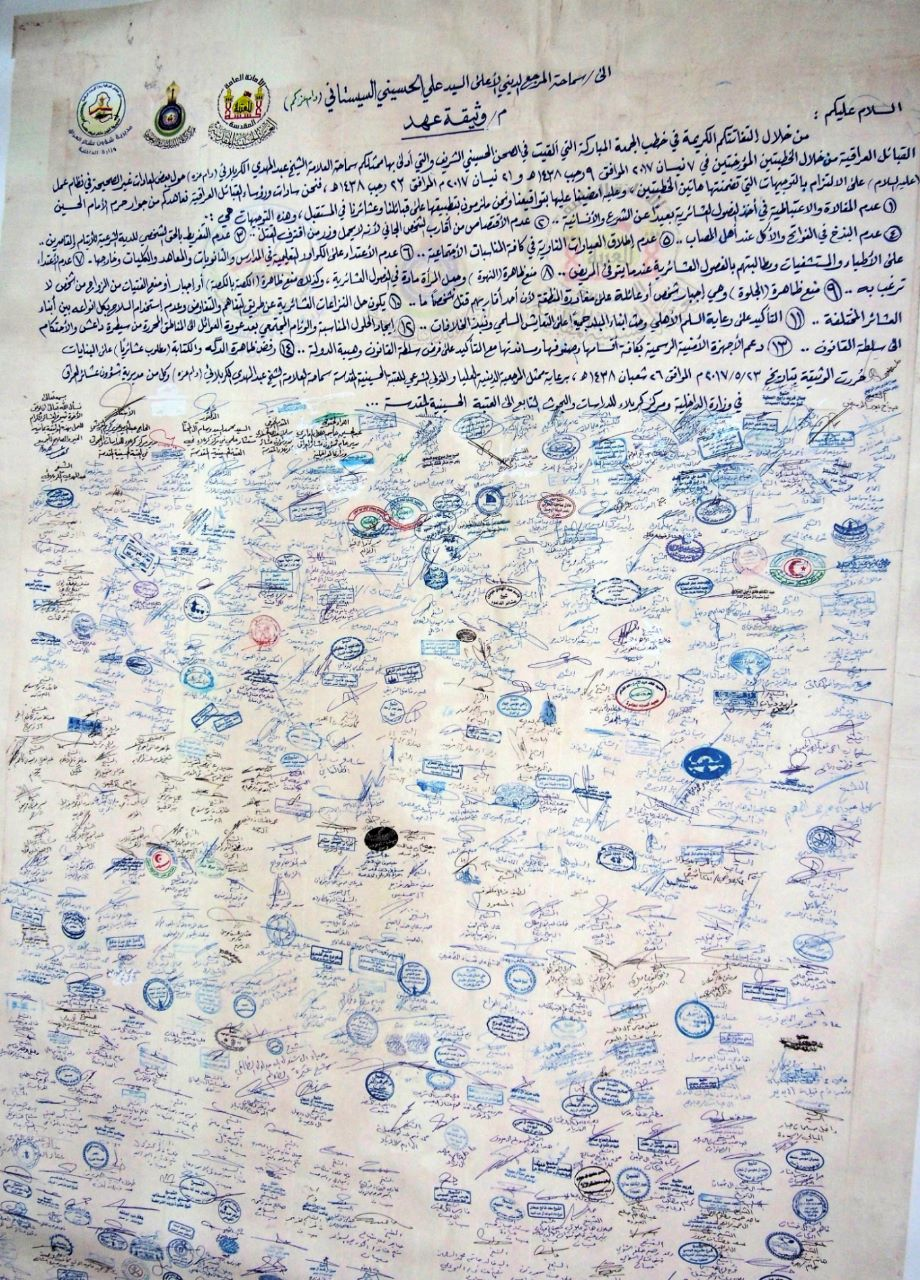
\includegraphics[height=0.5\textwidth]{images/karbala-honor-pact.jpeg}
% \label{fig:karbala-honor-pact}
% \end{figure}

The Honor Pact is a recent example of how Karbala entangles with tribal influence, politics, and religion. This complicates our typical understanding of clerical authority within south Iraq, complicating the notion that clerical authority can be easily translated into political authority. Marsin Alshamary has written about the concept of the "Najaf Veto", an often repeated trope from observers around election time \cite{alshamary_shia_2022}. While the veto captures the idea that there is an informal power the clerics have exercised in order to cross political hurdles and exert its influences, the signing of the Karbala Honor Pact shows that there are alternative means of expressing political authority beyond clerics. 

These tribal influences show that, historically, clerical authority has always been contested by other parties. Works that only focus on Najaf and the role of senior clerics misses how tribal influences have acted as a form of ethical self-fashioning outside of clerical guidance. 


\section{\emph{Muwālkib} Organization}
In Karbala, the most visible sign of this type of communal organization in guiding their own religious practices is in the \emph{muwālkib}. This chapter focuses on the intuition of the \emph{mūkeb} in Karbala, beginning by tracing the history of what the locals call the "Seven Great \emph{Muwālkib}", which represent the neighborhoods surrounding the shrine. These Seven perform a special religious ritual known as \emph{radat}, a type of procession combined with poetry. The history of the Seven is largely an oral history, and the \emph{radat} is an oral ritual which has been rarely discussed in English literature. To the best of my knowledge, after looking in the archives at the Center for Karbala Studies and the archives in the Karbala Central Library as well as various bookstores around town, I may be the first person to draw a map and record \emph{radat}s in recent history. The Seven Great \emph{Muwālkib} and their rituals provide an alternative frame to understanding how Karbalaeis articulate their understanding of their place in contemporary Iraqi society, and also shows that a clerical authority is under constant negotiation with local customs. 

A \emph{mūkeb} functions as the fundamental unit of organization for Shi’a rituals within Karbala. While not deemed specifically a Husseini ritual, the \emph{muwālkib} are responsible for organizing and providing services in order to facilitate the Husseini rituals. Villages around Karbala are typically organized alongside somewhat fluid tribal lines; the urban nature of Karbala changes the path of tribal organization. Instead, Karbalaeis organize themselves along \emph{beiyūtat}\footnote{This is already a double plural, \begin{Arabic}بيت\end{Arabic} is the singular form of the word "house", \begin{Arabic}
    بيوت
\end{Arabic} is the plural form of "houses. In order to distinguish the specific nominal meaning of "houses" or "clans", the Karbalaies have added the feminine plural ending of \begin{Arabic}
    -ات
\end{Arabic} onto a masculine plural word, forming \begin{Arabic}
    بيوتات
\end{Arabic}}, or houses. These houses in local neighborhoods often group together to form \emph{muwālkib}. The \emph{muwālkib} collect money from the affiliated houses and solicit outside donations in order to provide services for pilgrims, which religious devotees see as part of their duty to provide. 

\emph{Muwālkib} can also be from larger neighborhoods, such as the seven great \emph{muwālkib} of Karbala, explained later. The Hashd al-Shaabi also provides \emph{muwālkib} along the road from Najaf to Karbala. The manager of the Department of \emph{Muwālkib} describes this as:

\begin{quote}
    Anyone can start a \emph{mūkeb}...if someone wants to start a \emph{mūkeb} because they want to serve fish instead of lamb, they can go down the street and start a second [\emph{mūkeb}]. It is only in the city that we enforce licenses, because there is not enough space.
\end{quote}

A key function of the \emph{mūkeb} is to provide services for pilgrims in a tent. The term \emph{mūkeb} is used for both the tent and the organization itself. The tents can range from a single small tent with a stall providing basic food such as cheese and bread, to a full service tent providing sleeping space, cooked food, air conditioning, electricity, medical care, and foot massages. Many larger \emph{muwālkib} also provide space for rituals to be performed, although this may overlap with space that a \emph{husseiniyya} provides. It is not uncommon to see a \emph{husseiniyya}'s courtyard be filled with a particular family's \emph{mūkeb}, which provides food and other services. 

During the day before Ashura, as well as the week leading up to Arbaeen, the area around the two shrines is filled with \emph{muwālkib}. The Department of Muwalkib, run by the shrine of Abbas, is responsible for providing licenses and other various logistical efforts in supporting \emph{muwālkib} around the city.

\section{Department of \emph{Muwālkib}}
The department of \emph{Muwālkib} occupies a two story building tucked away in an alleyway close to the Shrine of Abbas, next to the shrine known as the "Left Hand of Abbas" \footnote{In the battle of Karbala, Abbas's hands were cut off, and there are two separate minor shrines known as the Left Hand of Abbas and the Right Hand of Abbas. These two shrines serve as additional visitation sites, one can often see women and men lamenting and performing \emph{latm} in front of these sites.}. 

The department of \emph{Muwālkib} was a repeated fieldwork site for me, I repeatedly visited the manager and other bureaucrats who ran the operation. During an interview with the manager of the department, who agreed to interviews but asked to not be specifically named in any English publication, the manager described that there were over 3,000 \emph{muwālkib} providing services within the city limits of Karbala, with around 200 providing sites to perform Majlis al-'aza. The department's primary role is to facilitate licenses to the 3,000 within city limits. The only exception to this licensing are \emph{muwālkib} affiliated with the Seven Great \emph{Muwālkib}, which I describe later in this chapter. 

% The licenses are issued as physical ID cards, with Arabic on one side and English on the other. These cards identify the typical information such as name, \emph{mūkeb} name, expiration, and so on. The licences bear the logos of both \emph{atabat}, although everyone working in the department was an employee of the al-Kafeel foundation, the \emph{ataba} for the Shrine of Abbas.

% \begin{figure}[!tbp] \label{fig:mowkeb-liscense}
%   \centering
%   \subfloat[Front side]{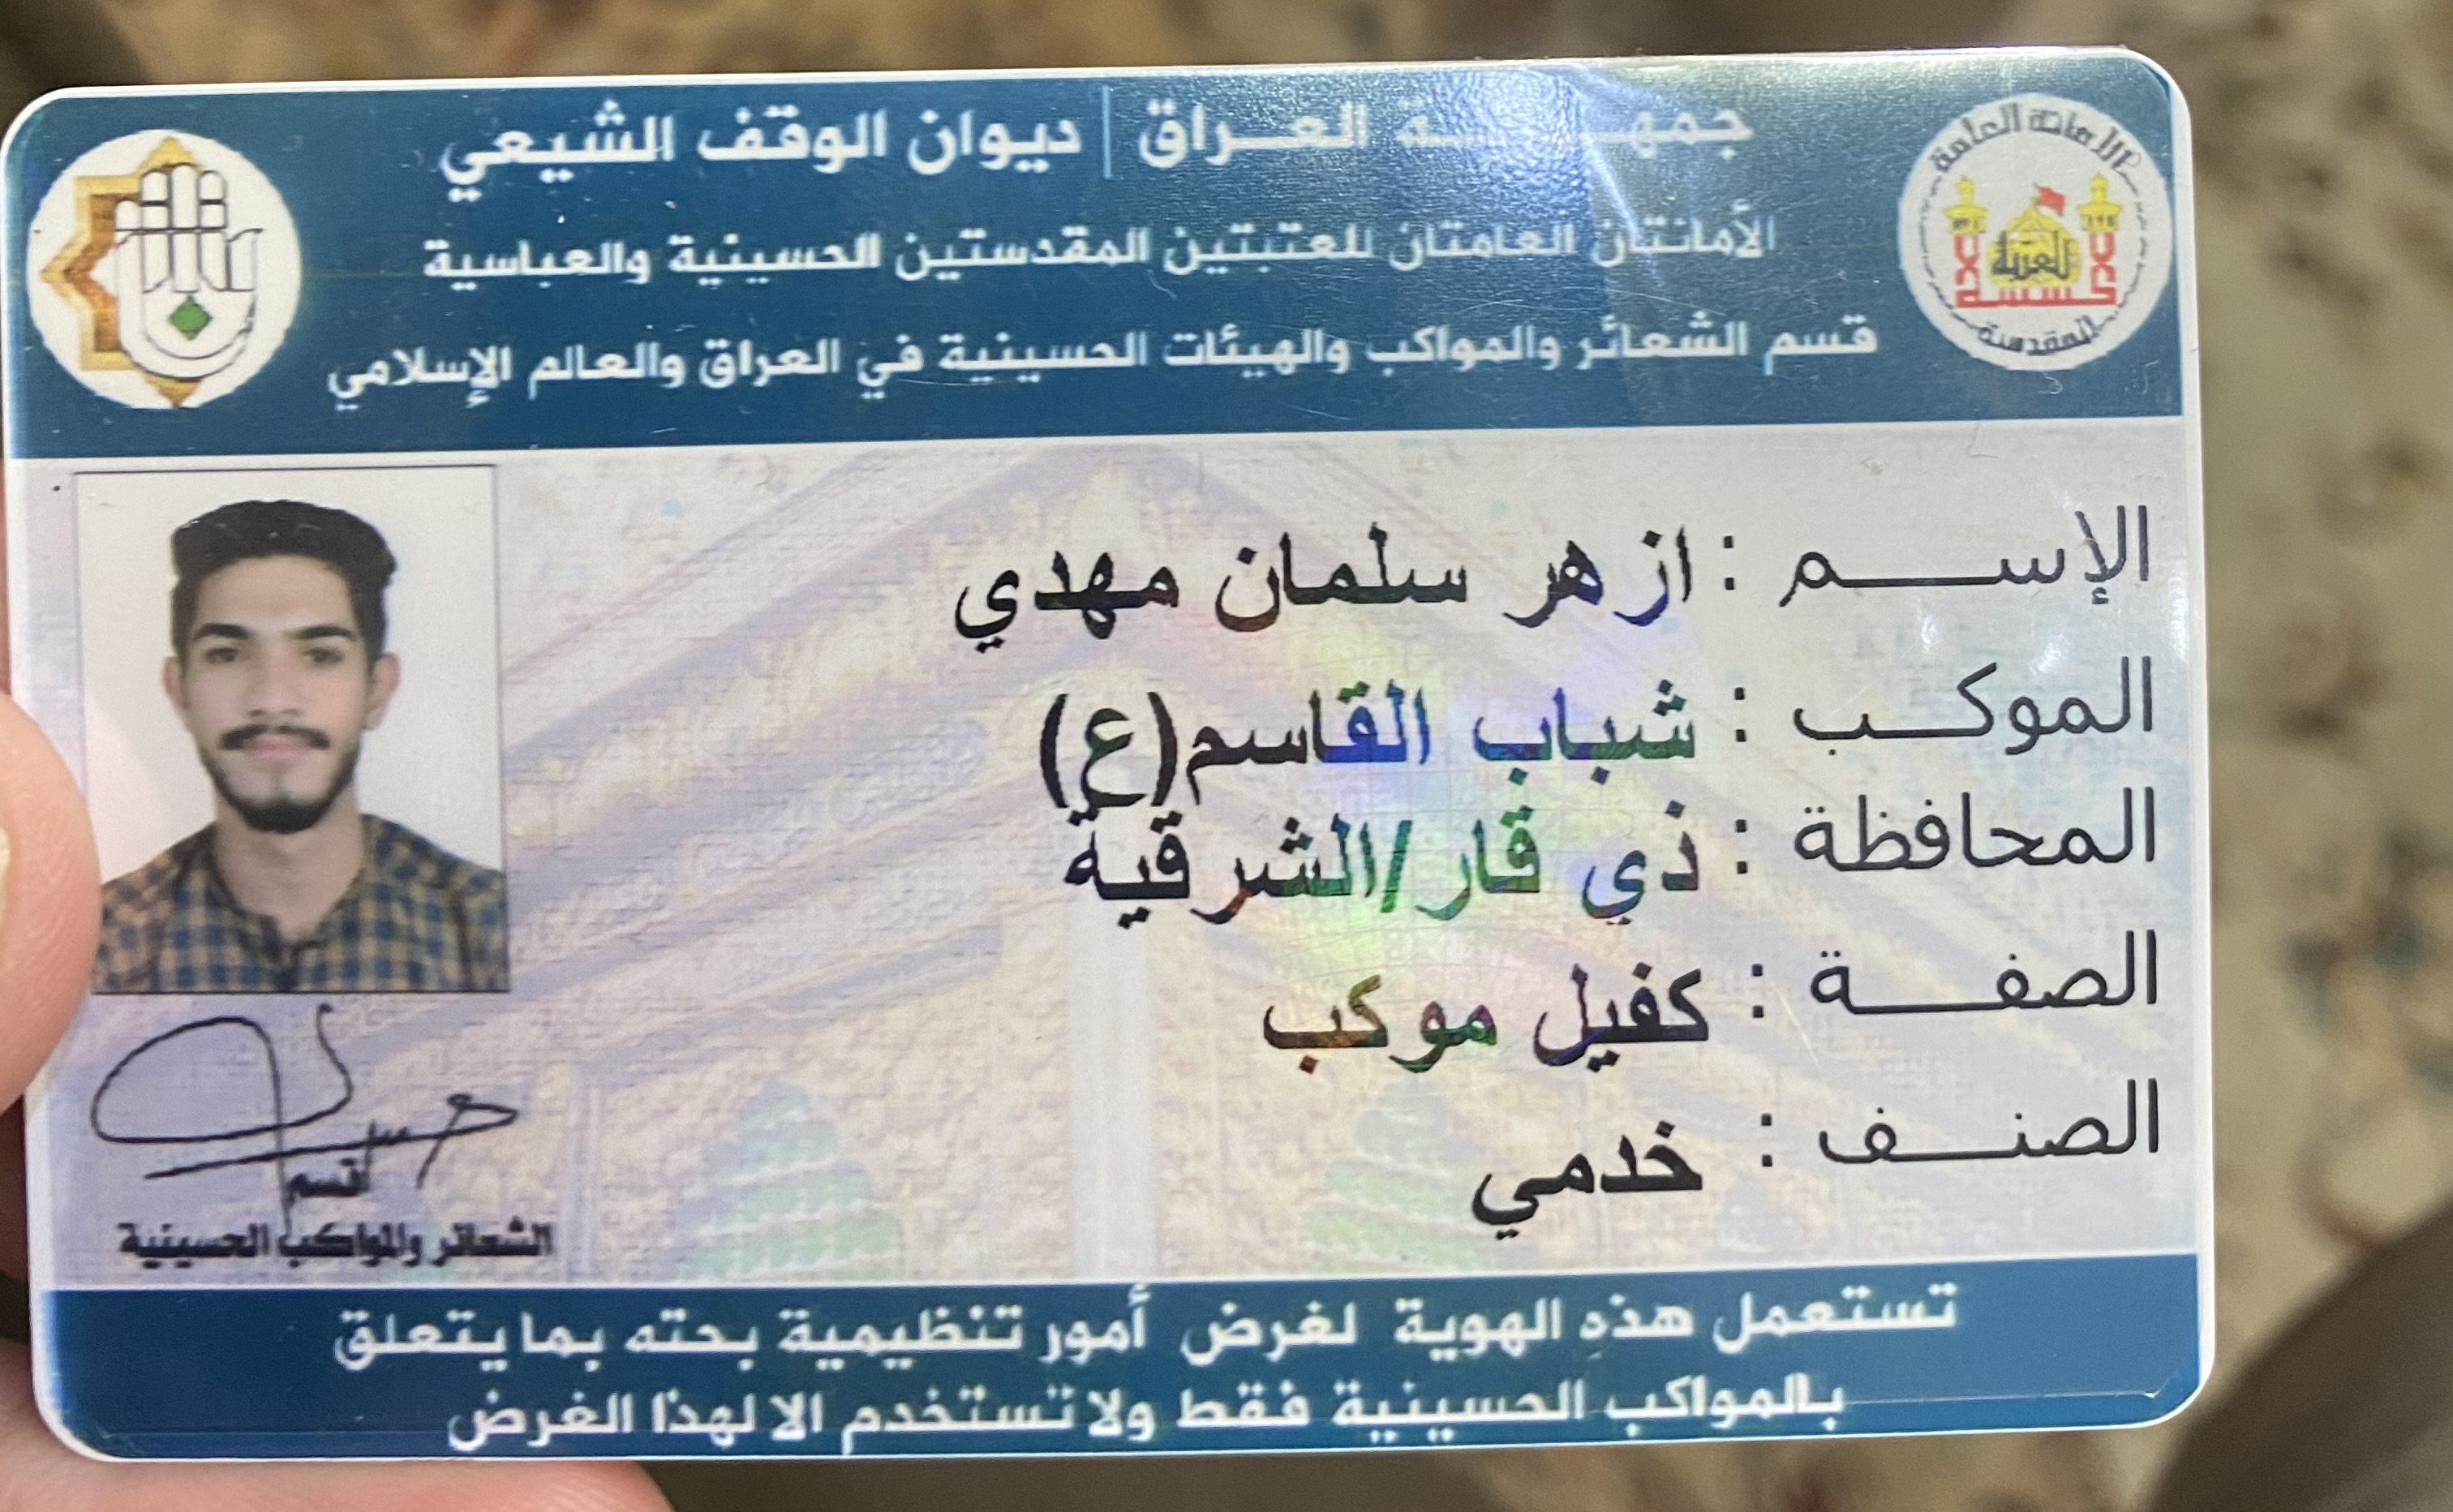
\includegraphics[width=0.4\textwidth]{images/mowkeb-liscense-front.jpeg}\label{fig:f1}}
%   \hfill
%   \subfloat[Back side]{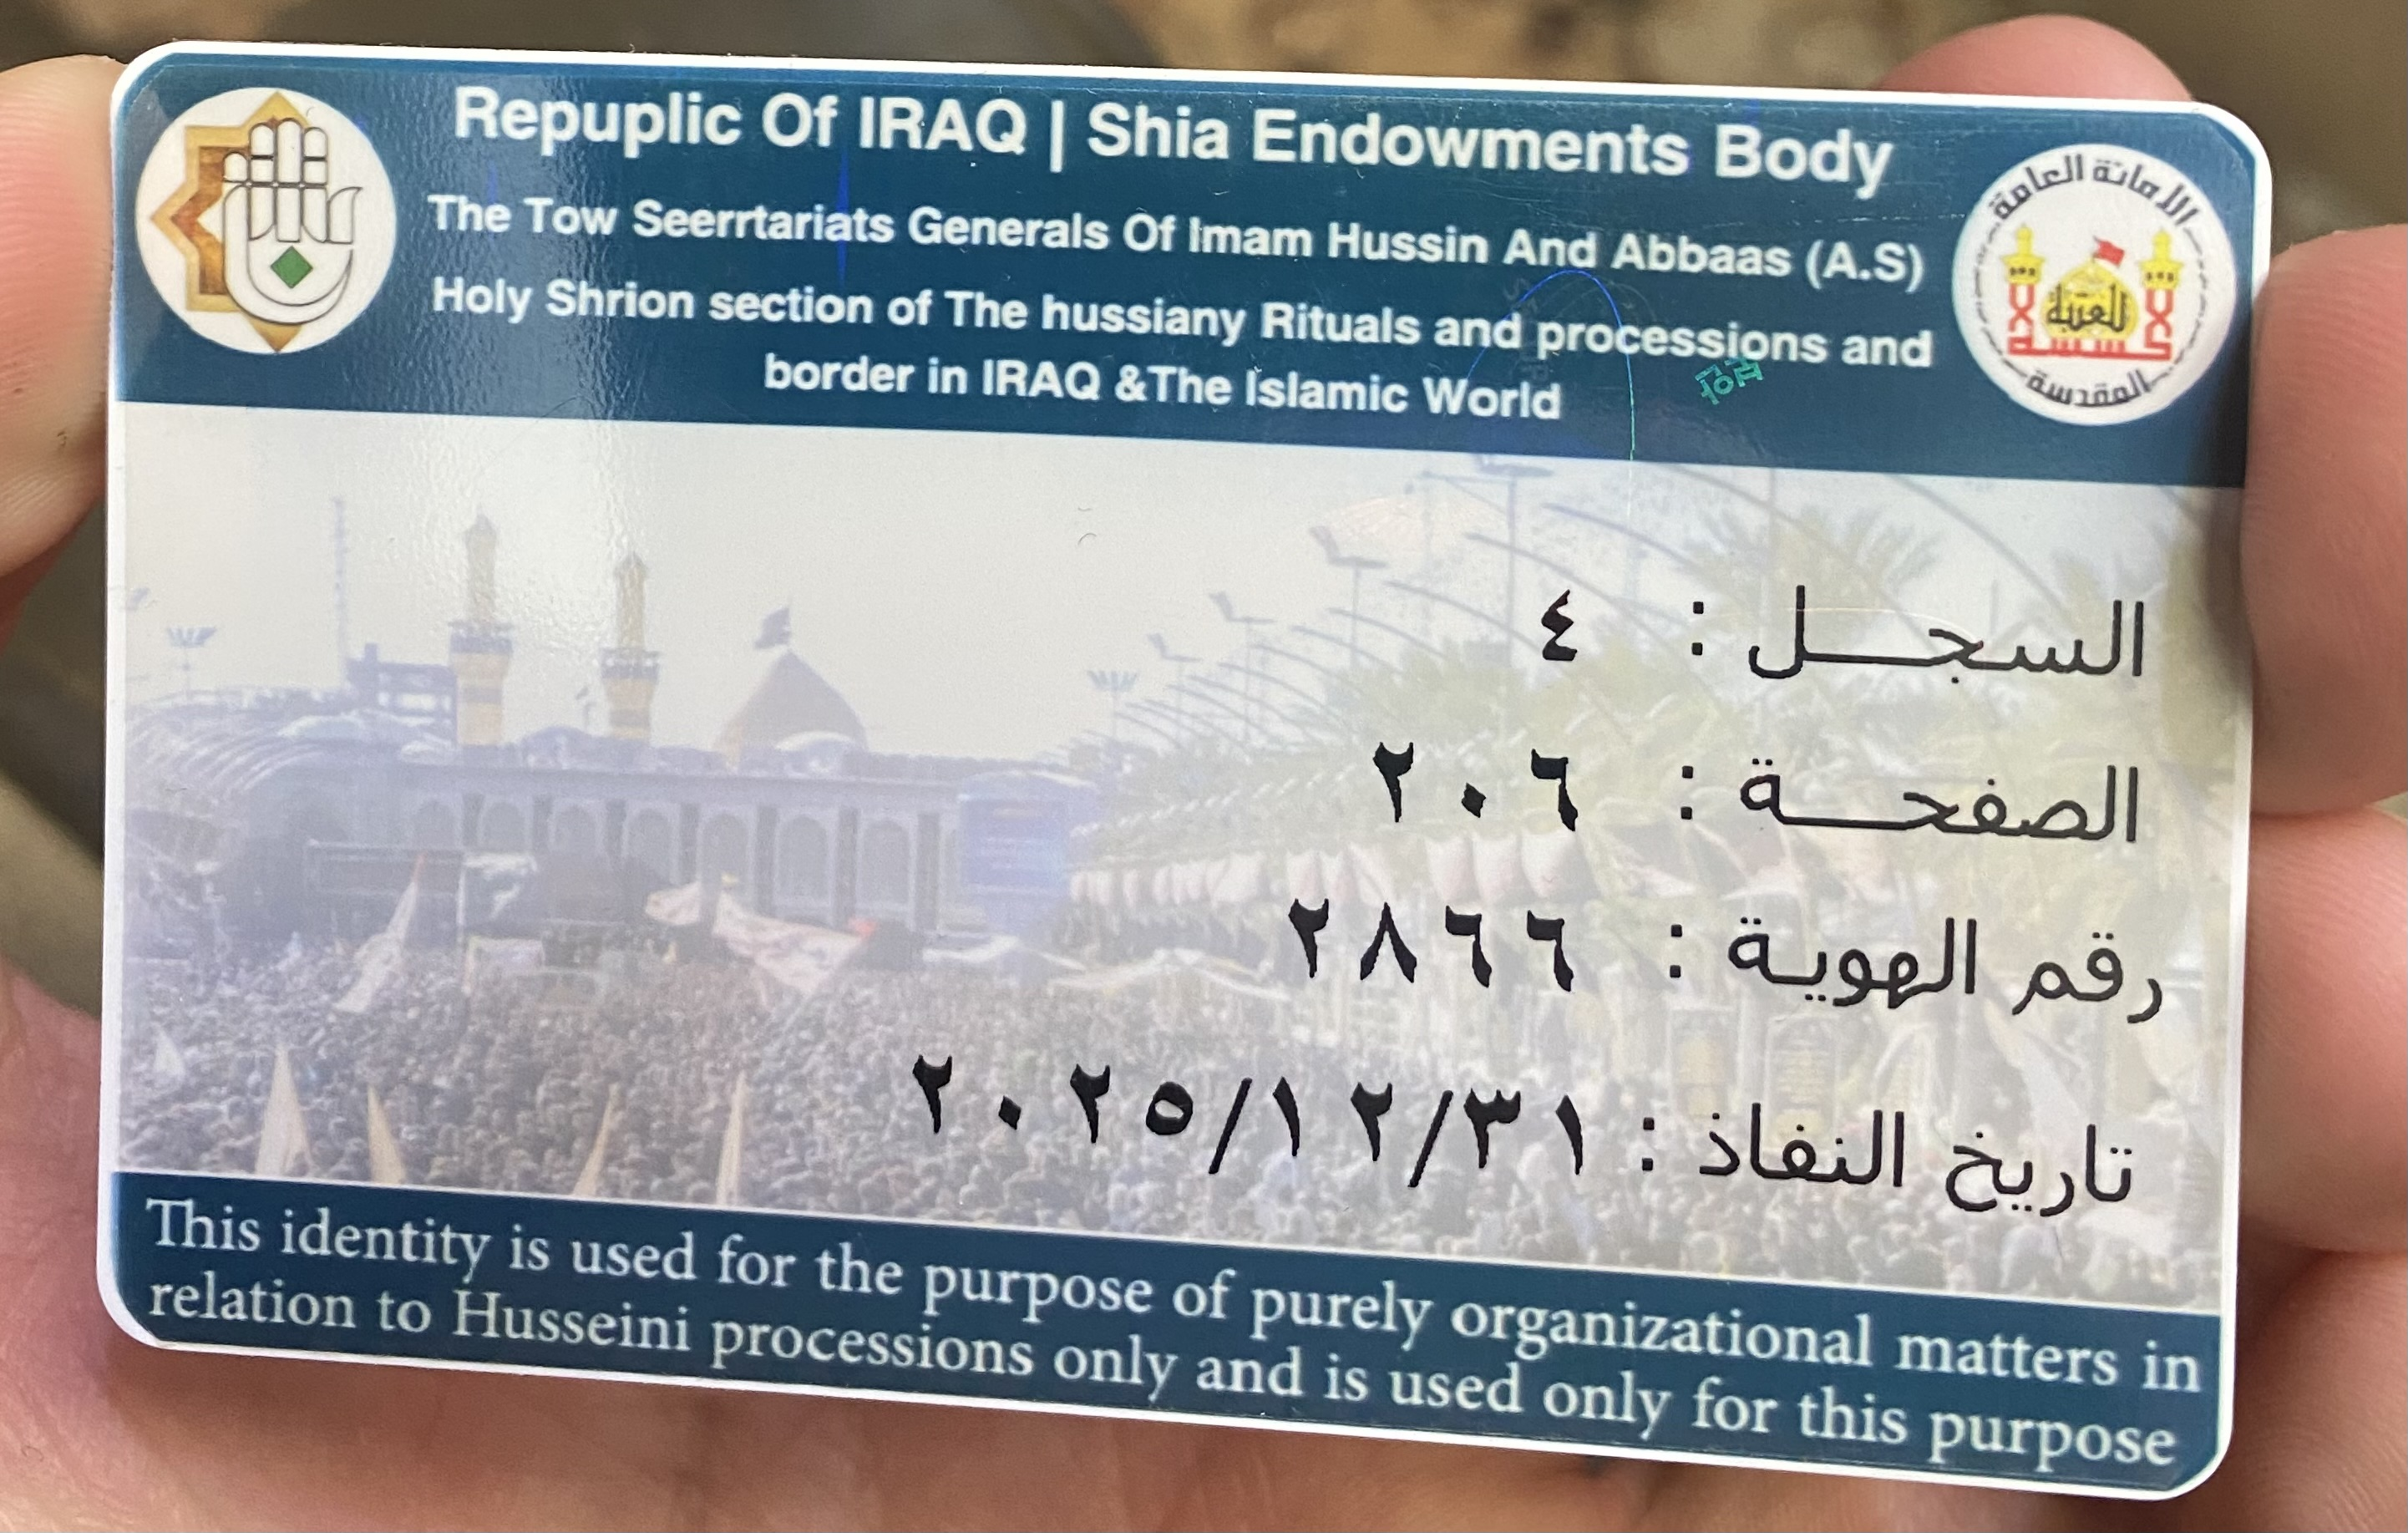
\includegraphics[width=0.4\textwidth]{images/mowkeb-licsense-back.jpeg}\label{fig:f2}}
%   \caption{A \emph{mūkeb} licsense issued from the Department of Muwālkib. Photo taken with the permission of the department in March 2022.}
% \end{figure}

Department workers were generally reluctant to provide interviews to me without assurances that I was not a journalist. The relatively recent BBC scandal mentioned in the introduction has caused every department to become more suspicious of foreigners asking questions, and it took over three months of repeated engagements before anyone besides the manager was willing to talk to me. However, I noticed that even after multiple workers had become accustomed to me, none, including the manager, was willing to provide an explanation for why the al-Kafeel foundation was solely responsible for running the department. Questions would often elicit non-answers such as "events happened this way" followed by signs that I should ask different questions. 

% \subsection{Schools of Thought (Shirazi, Iranian, Qaziwini, etc)}
% Among the many \emph{muwālkib} are the different schools of thought. Each \emph{mūkeb} is affiliated with not only a particular neighborhood, but the traditions of the neighborhood itself influences the political nature of rituals. For example, on the Qibla road leading towards the Shrine of Imam Hussein, multiple mokwebs can be see bearing the pictures of Ayatolla Sadiq Shirazi. Another popular \emph{mūkeb} is run by the family of Ayatollah Qazwini, which runs Husseiniya Qazwini, whose popularity in the United States has helped popularize the \emph{mūkeb} itself. 

% The \emph{muwālkib} are highly political as well, with many affiliated with the Hashd al-Shaabi. Opinions of the Hashd range from them being Iranian proxies to defenders of the faith, with many \emph{muwālkib} along the road creating mock graves for Abu Mahdi Muhandis and Qassem Soleimani. 

\section{The Seven Great \emph{Muwālkib}} \label{seven-great-mokwebs}
Although \emph{muwālkib} function as a unit of organization, the seven great \emph{muwālkib} have grown to encompass entire neighborhoods. Originally the seven neighborhoods surrounding the shrines of Karbala, each has developed into a distinct neighborhood with its personalities \ref{fig:mowalkib} in the old city. During my fieldwork, I walked with a member of each neighborhood in order to map out the boundaries on each \emph{mūkeb}. During Muharram, members of each neighborhood gather into their specific \emph{mūkeb}, with each \emph{mūkeb} performing a procession between the shrines of Imam Hussein and Abbas. In clockwise order they are:  Mukeb Taraf Bab Baghdad, Mukeb Bab al-Khan, Mukeb Taraf Bab al-Najaf, Mukeb Taraf Bab Abbasiyya, Mukeb Taraf Bab al-Mukhaym, Mukeb Taraf Bab al-Taq, and Mukeb Taraf Bab al-Salam.

As each of the seven great \emph{muwālkib} trace their roots to the founding of Karbala, their boundaries have been built into the roads of the city. The major highways leading to Baghdad and Najaf were built around the \emph{mūkeb}-neighborhoods themselves, leaving the \emph{mūkeb} divisions within the architecture of the city itself. 

\begin{figure}[H]
\caption{The seven great \emph{muwālkib} of Karbala. Exact neighborhood streets are subject to change occasionally, these represent the rough boundaries on each \emph{mūkeb} neighborhood. Map made from author's fieldwork.}
\centering
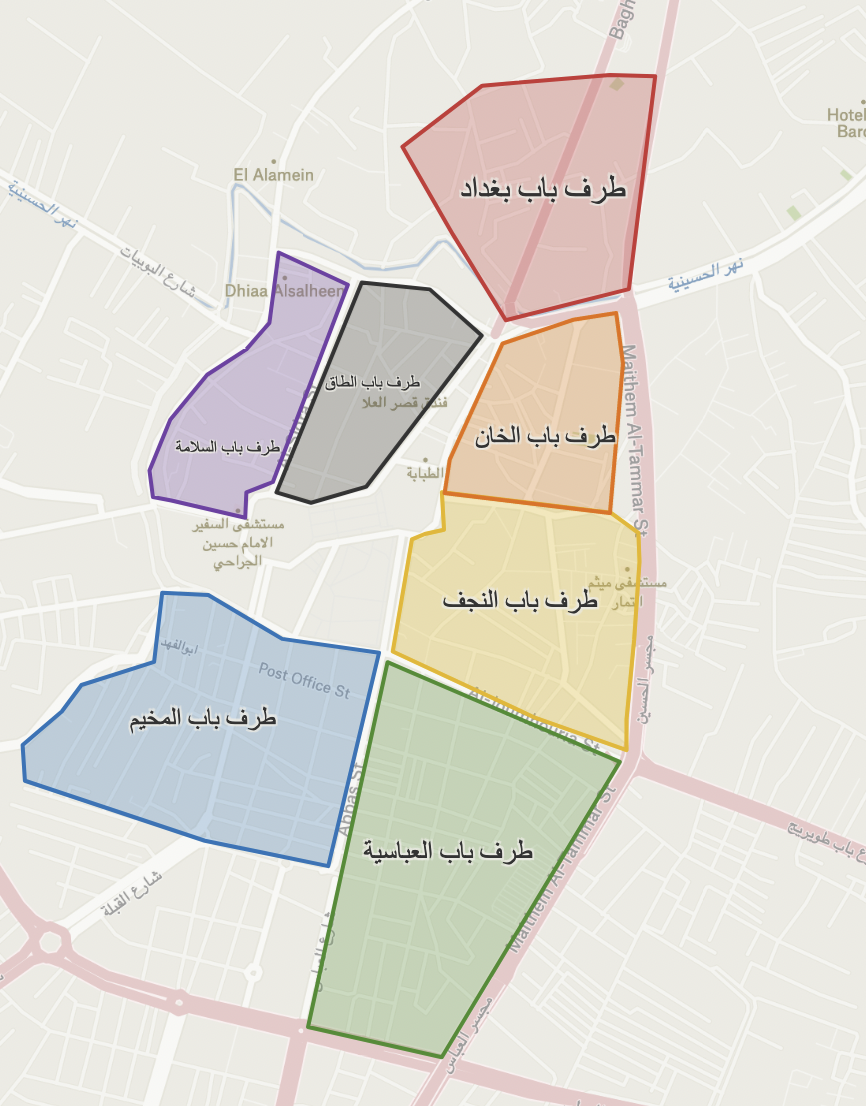
\includegraphics[height=0.75\textwidth]{images/seven-mowkebs.png}
\label{fig:mowalkib}
\end{figure}

Mukeb Taraf Abbasiyya is the most politically active \emph{mūkeb}, with many interviewees claiming that they are communist. While it is unclear how many communists actually resided in the neighborhood or were affiliated with the \emph{mūkeb} in the neighborhood as local records are not clear, the \emph{mūkeb} procession of Taraf Abbasiyya is known to be more political than the others, especially \emph{radat}. In contrast to Mukeb Taraf Abbasiyya is Mukeb Bab al-Najaf, whose \emph{radat} is perceived to be purely religious. Several of the same interviewees who described Mukeb Taraf Abbasiyya as communist went on to describe how Mukeb Bab al-Najaf only performs religious \emph{radat}. 

\section{\emph{Radat}}
A special ritual is conducted by the Seven Great \emph{muwālkib}, known as Radat Siyasi Karbalaei, translated as "the radat of Karbalaei politics". A \emph{radat} is a marching procession: a banner leads a group, followed by a second group carrying a \emph{howdej}, followed by multiple groups chanting sections of a poem. The march begins at the outer gates of the Shrine of Abbas, then proceeds to \emph{bayn haramayn}, and finally proceeds into the Shrine of Hussein, where all the ritual attendees gather for a \emph{latm} performed by a \emph{radūd} affiliated with the specific \emph{mūkeb}. Immediately behind the last group of one \emph{mūkeb} is the banner of another \emph{mūkeb}. 

Performed only during the third to the ninth of Muharram, the \emph{radat} is only performed by people belonging to specific Karbala neighborhoods. Because the vast majority of pilgrims arrive either on the ninth of Muharram or the two weeks leading up to Arbaeen, the vast majority of pilgrims are not aware of \emph{radat}. In my interviews with Iranian and Pakistani pilgrims, many of them expressed that they had never seen this ritual. 

The banner announces which \emph{mūkeb} the procession is affiliated with. The banner is an ornately decorated banner, held by two men, which spells out “\emph{mūkeb} X” in Arabic (see figure \ref{fig:taraf-abbiyya-banner}). Oftentimes this is accompanied by flags afterwards, which may be Iraqi flags, flags relating to Shi'a Islam, or flags of various Islamic colors. Multiple \emph{muwālkib} had flags bearing “Ya Hussein” or the Iraqi flag itself, which presents an interesting contrast of nationalism and religion. 

Following the flags is usually the \emph{howdej}: a 70 kilogram boat that is often carried by a single man (see figure \ref{fig:howdej}). A hadith from the prophet described Imam Hussein as the light of salvation, leading Shi'as to construct a metal boat of lamps. Either electric or gas-lit, the \emph{howdej} is a mainstay of Shi'a rituals between the third of Muharram to the ninth of Muharram. Cries of mourning can be heard as they carry the \emph{howdej}, with subsequent chants of "ya Allah!" or "ya Ali!". The \emph{howdej} itself is adorned with lights in the shape of a pyramid, crowned with a wreath at the top, representing Hussein. Two snake-like creatures flank the ends of the ship, with their open mouths turned towards the pyramid of light, representing the evil that lurks and the danger the world bears towards Hussein. 

\begin{figure}[H] \label{fig:radat-pics}
  \centering
  \subfloat[The banner of Mukeb Taraf Abbasiyya. The \emph{howdej} and chants follow in separate groups.]{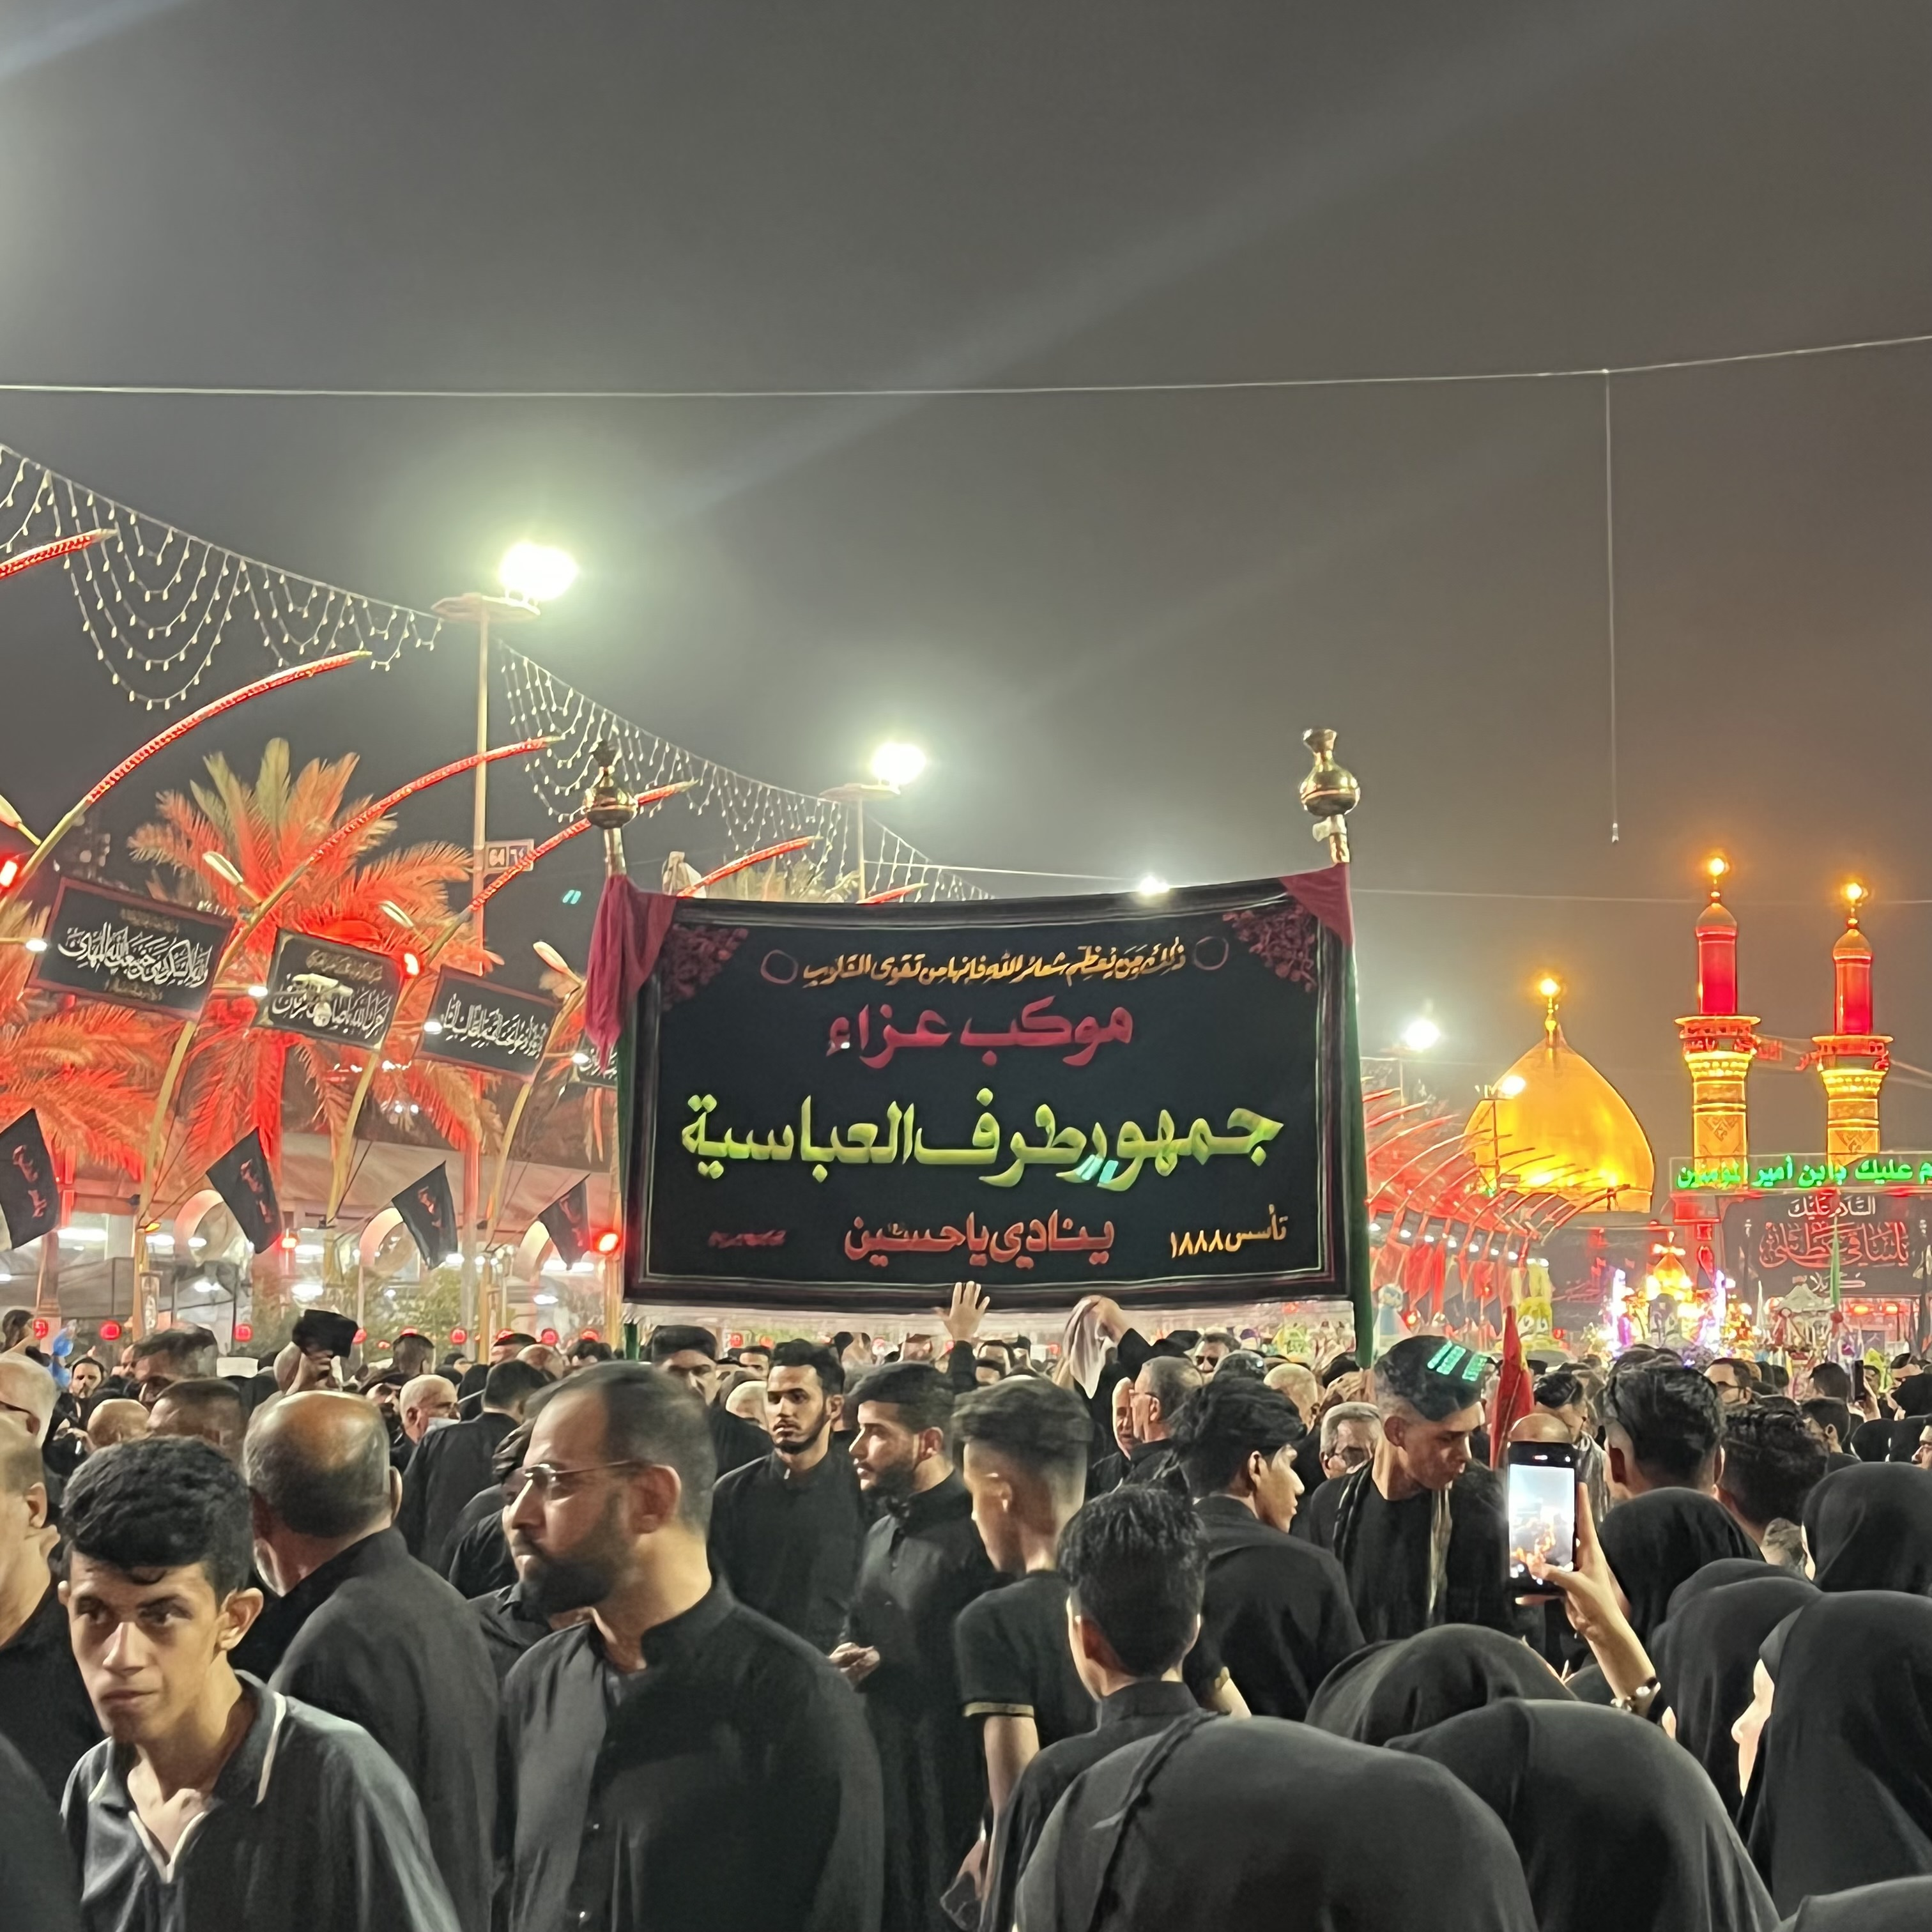
\includegraphics[width=0.4\textwidth]{images/mokweb-abasiyya/banner.jpeg}\label{fig:taraf-abbiyya-banner}}
  \hfill
  \subfloat[A \emph{howdej} being carried in between the two shrines.]{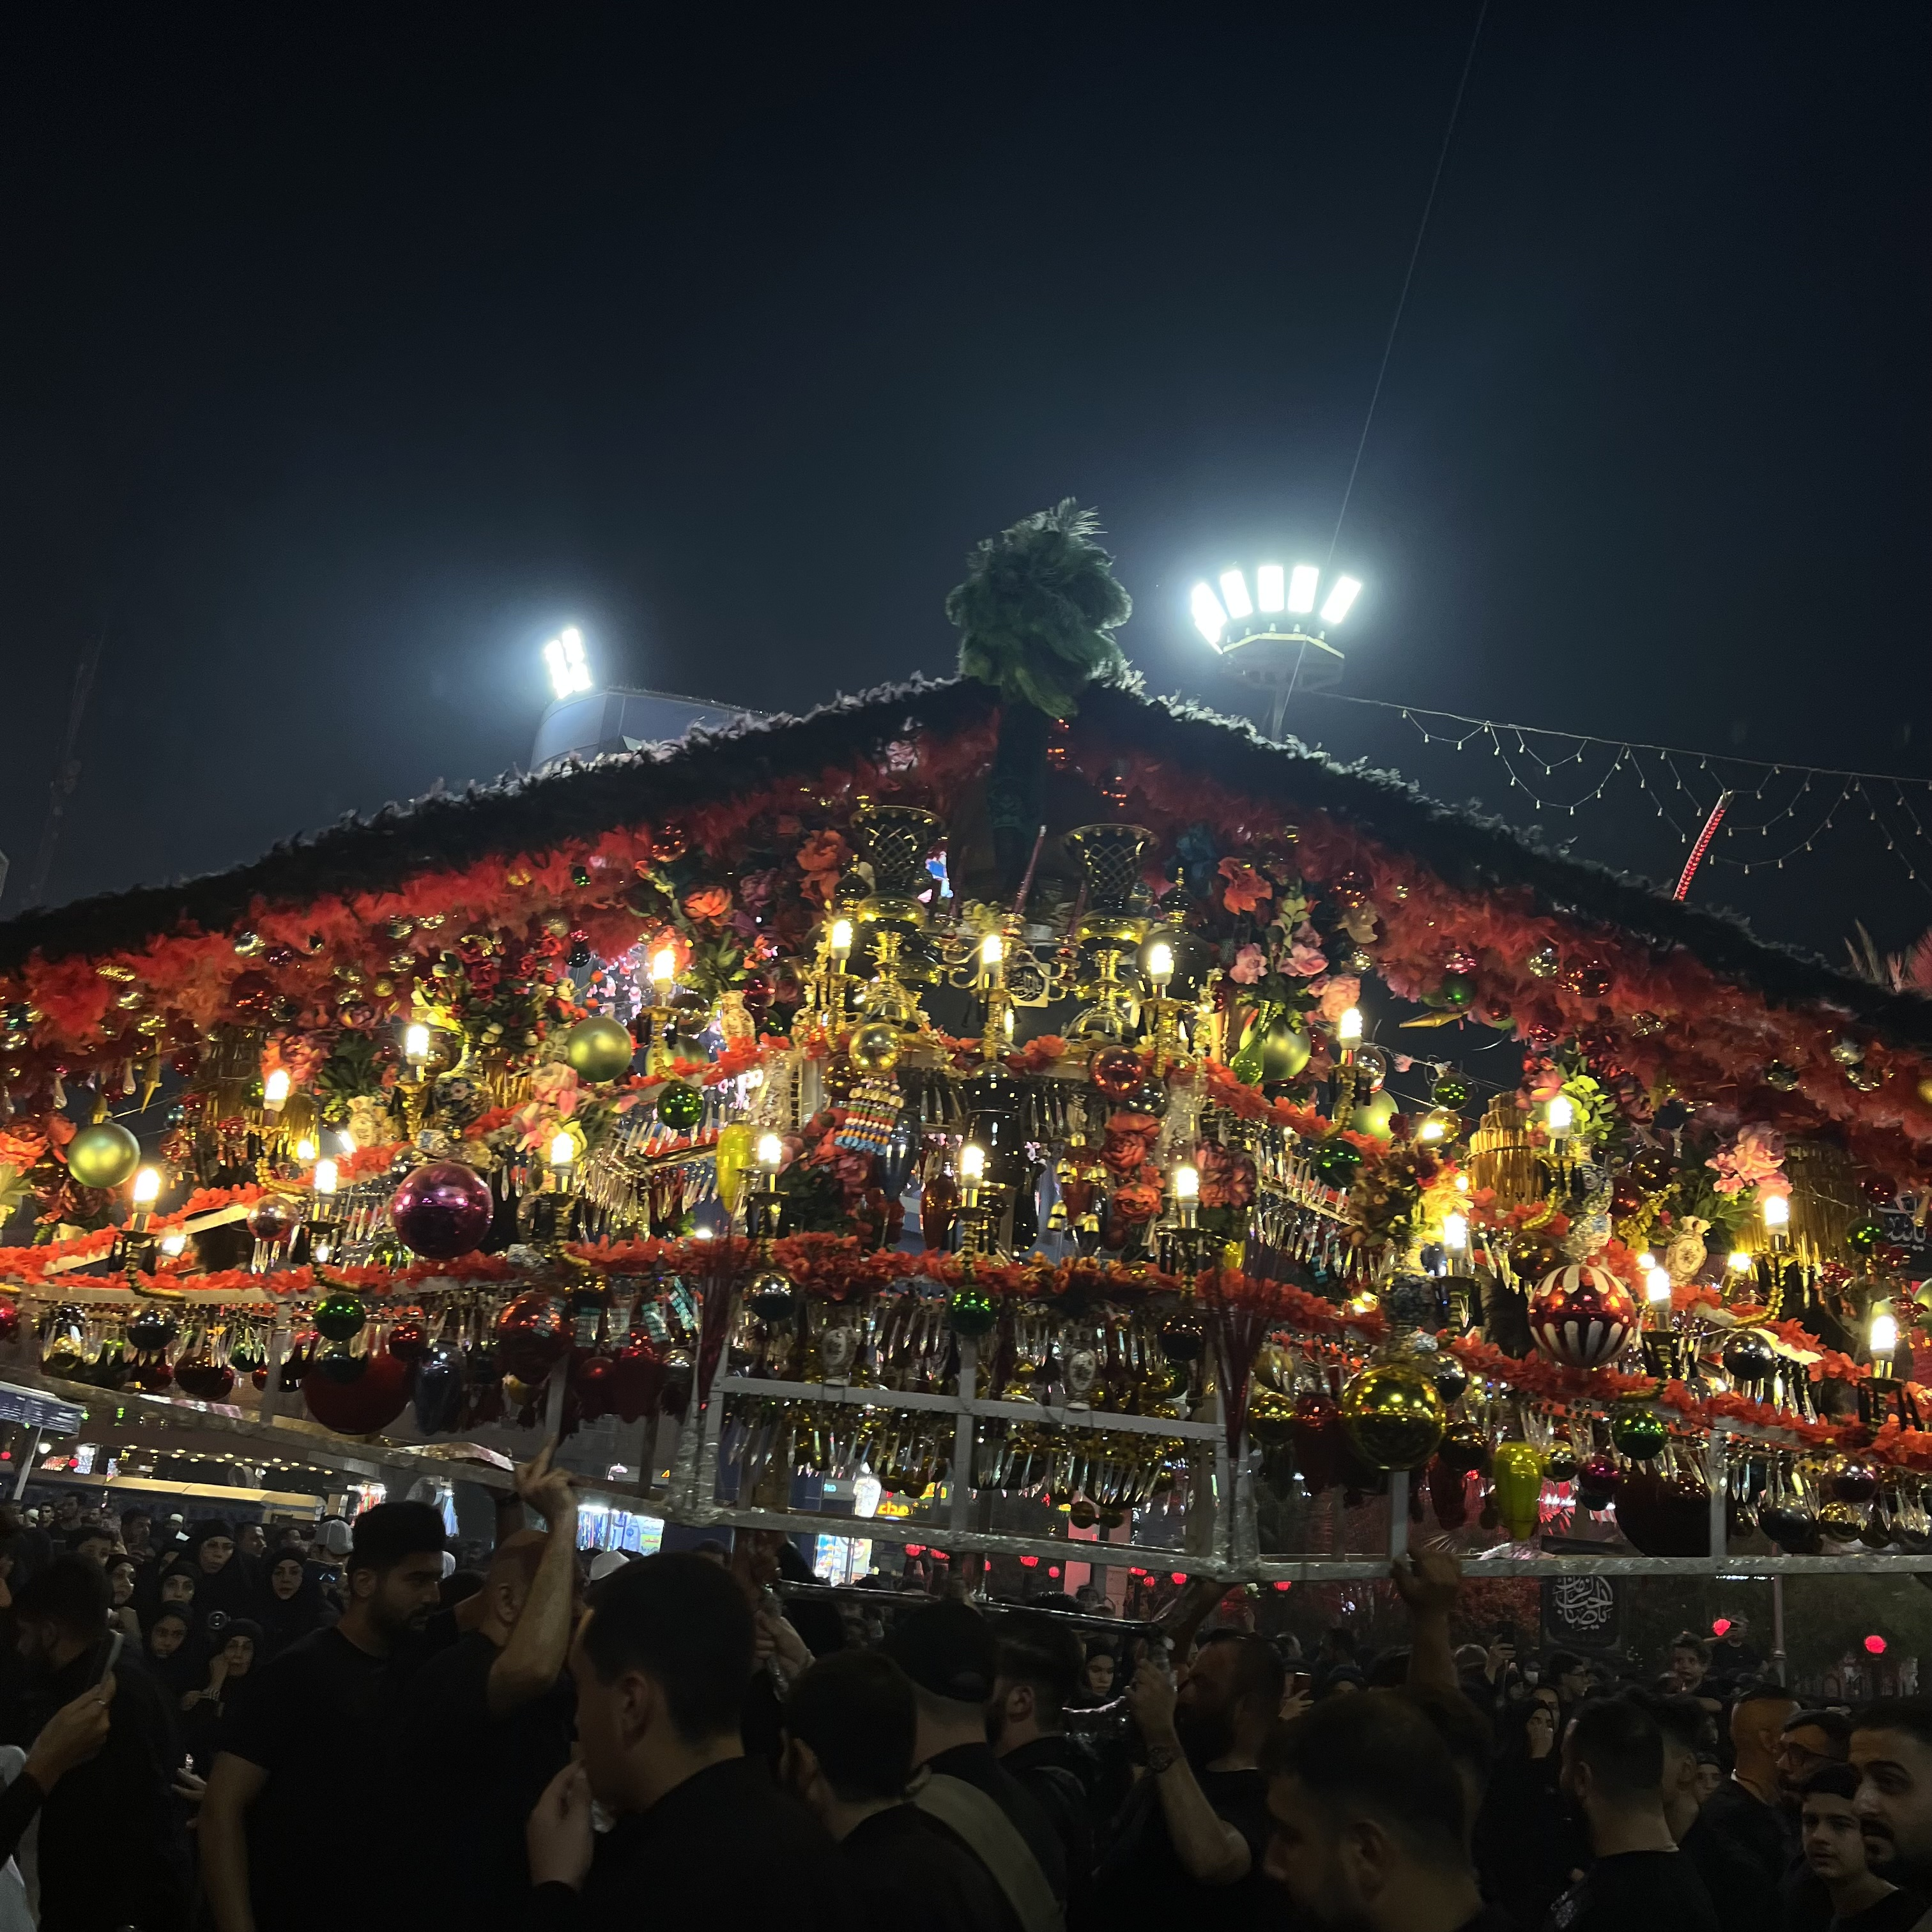
\includegraphics[width=0.4\textwidth]{images/mokweb-abasiyya/howdej.jpeg}\label{fig:howdej}}
  \hfill
\subfloat[Members of Mukeb Taraf Abbasiyya chanting a section of a poem as they enter the Shrine of Imam Hussein. The chant follows a specific meter, which participants wave their hands to. ]{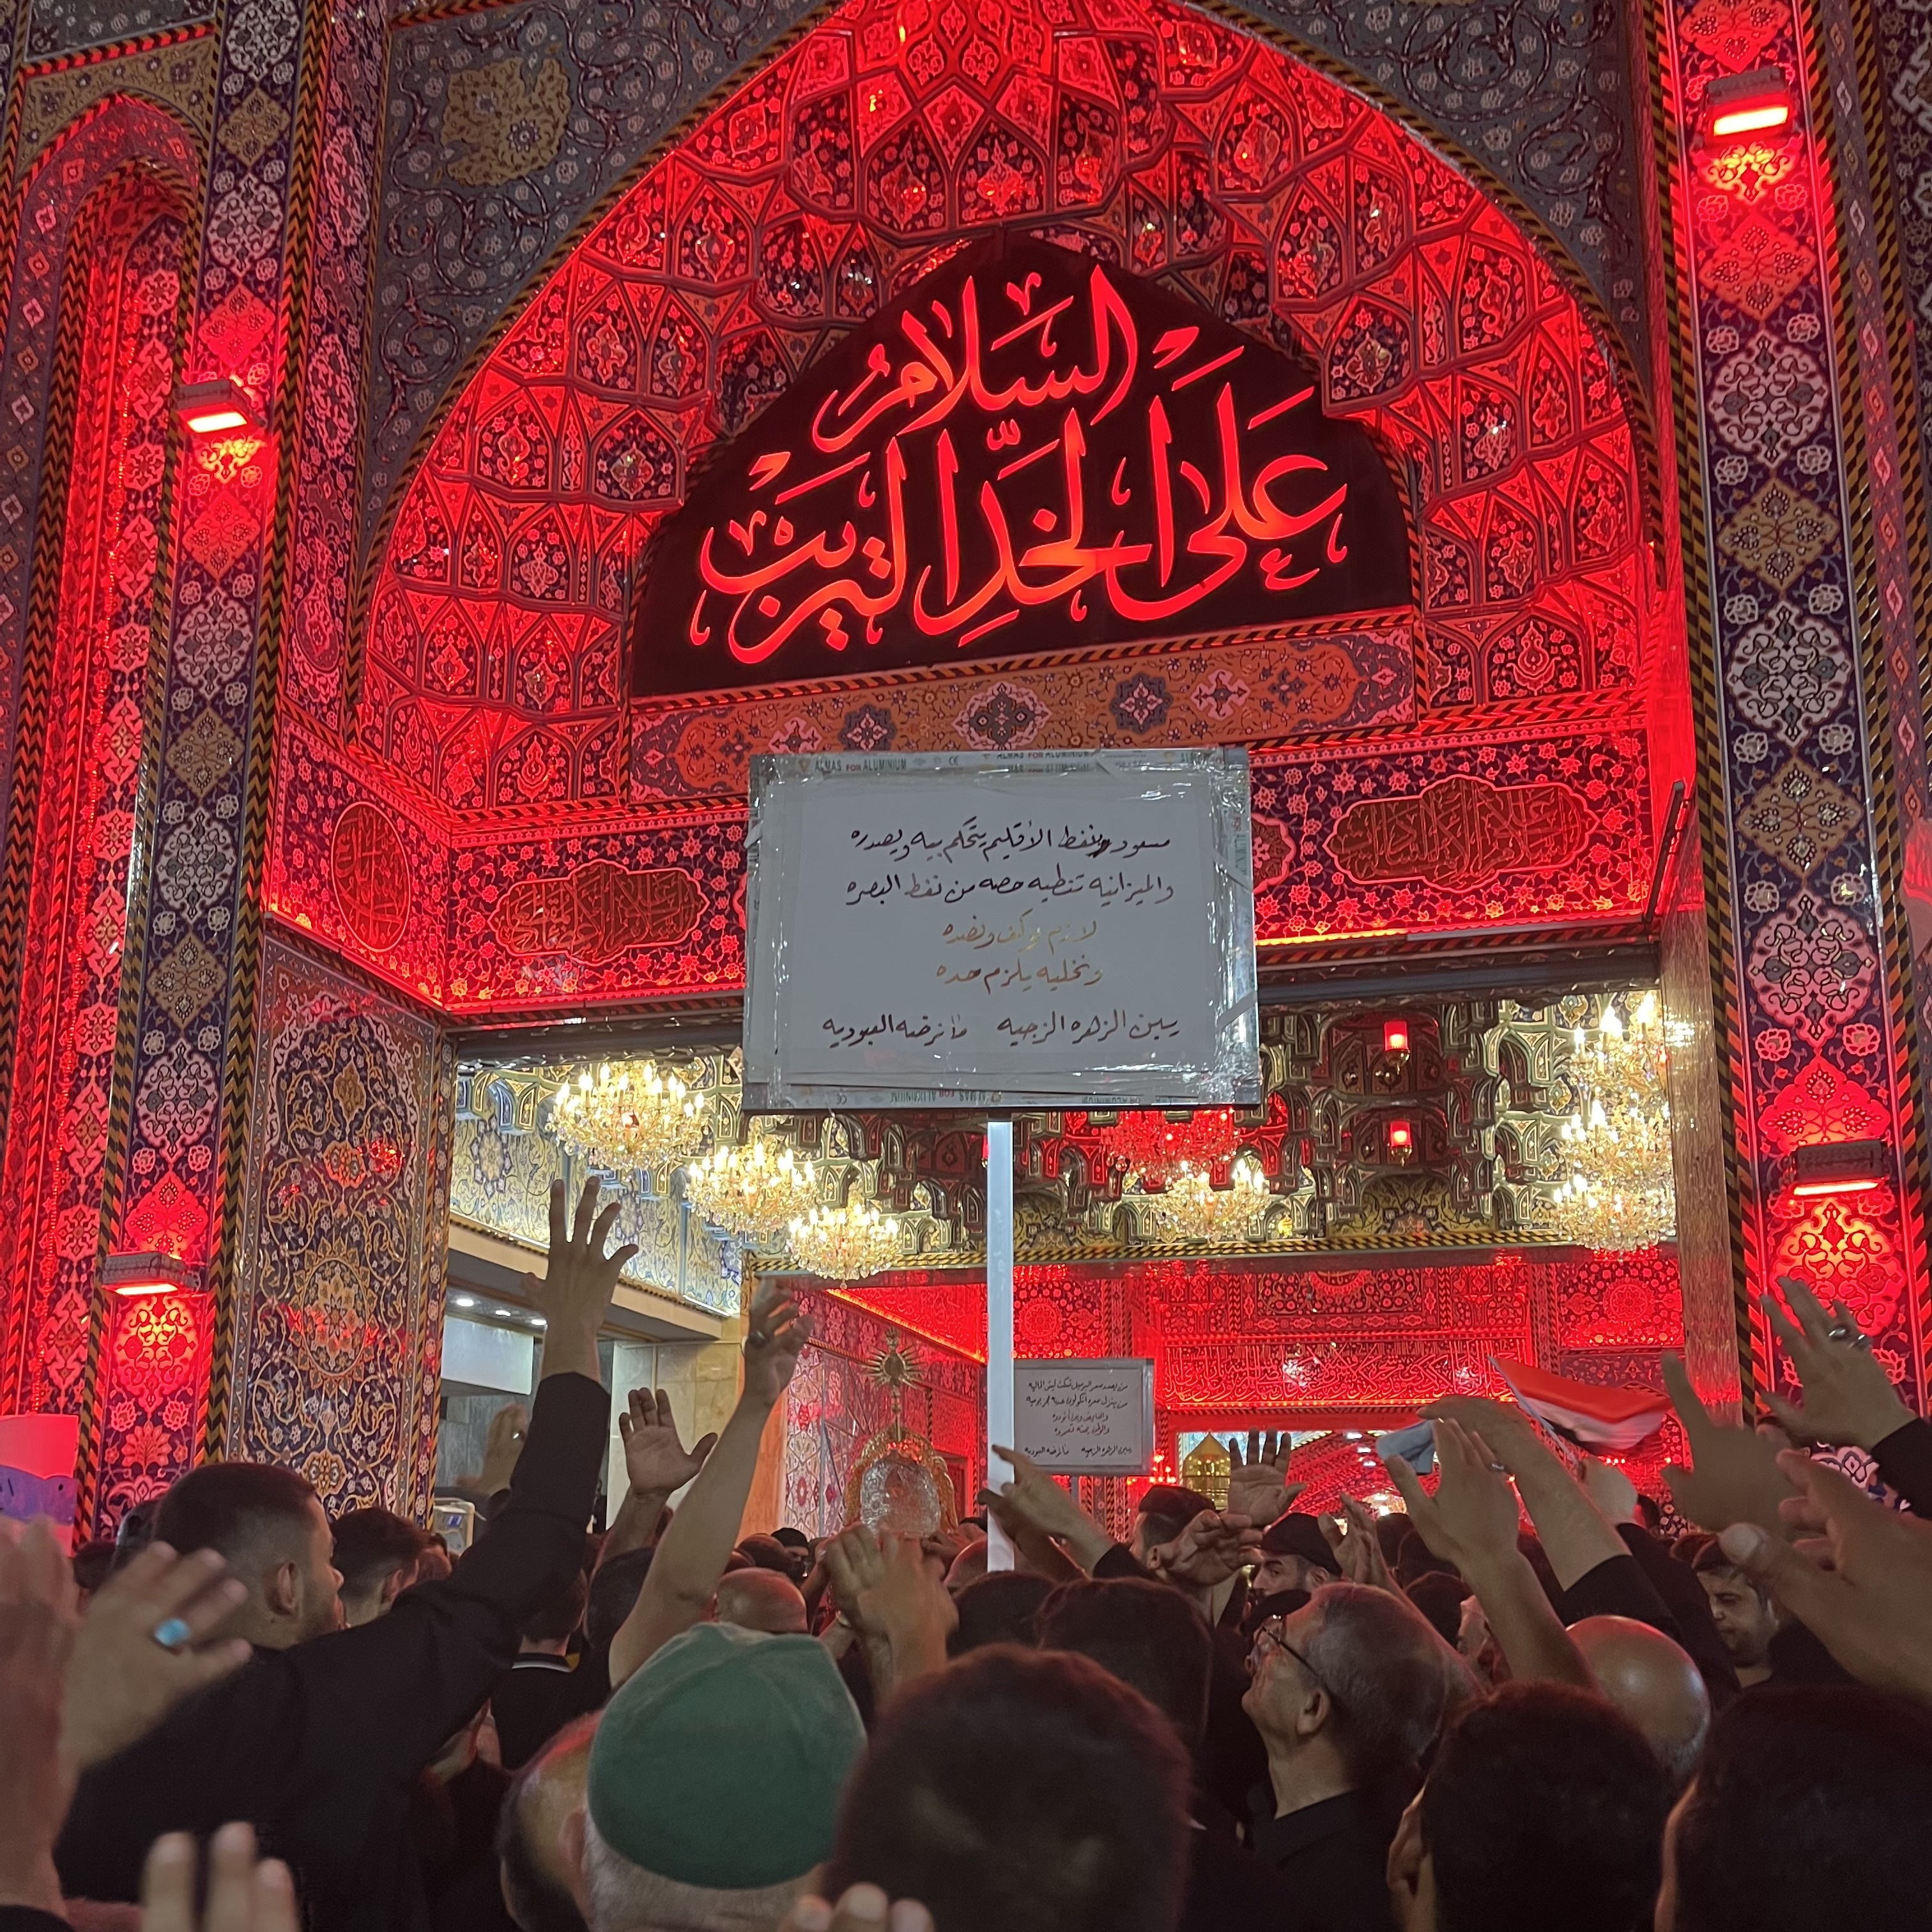
\includegraphics[width=0.4\textwidth]{images/mokweb-abasiyya/chant.jpeg}\label{fig:radat-chanting}}
  \hfill
  \subfloat[A young man holds the sign with a poem section for members of Mukeb Taraf Abbasiyya to read.]{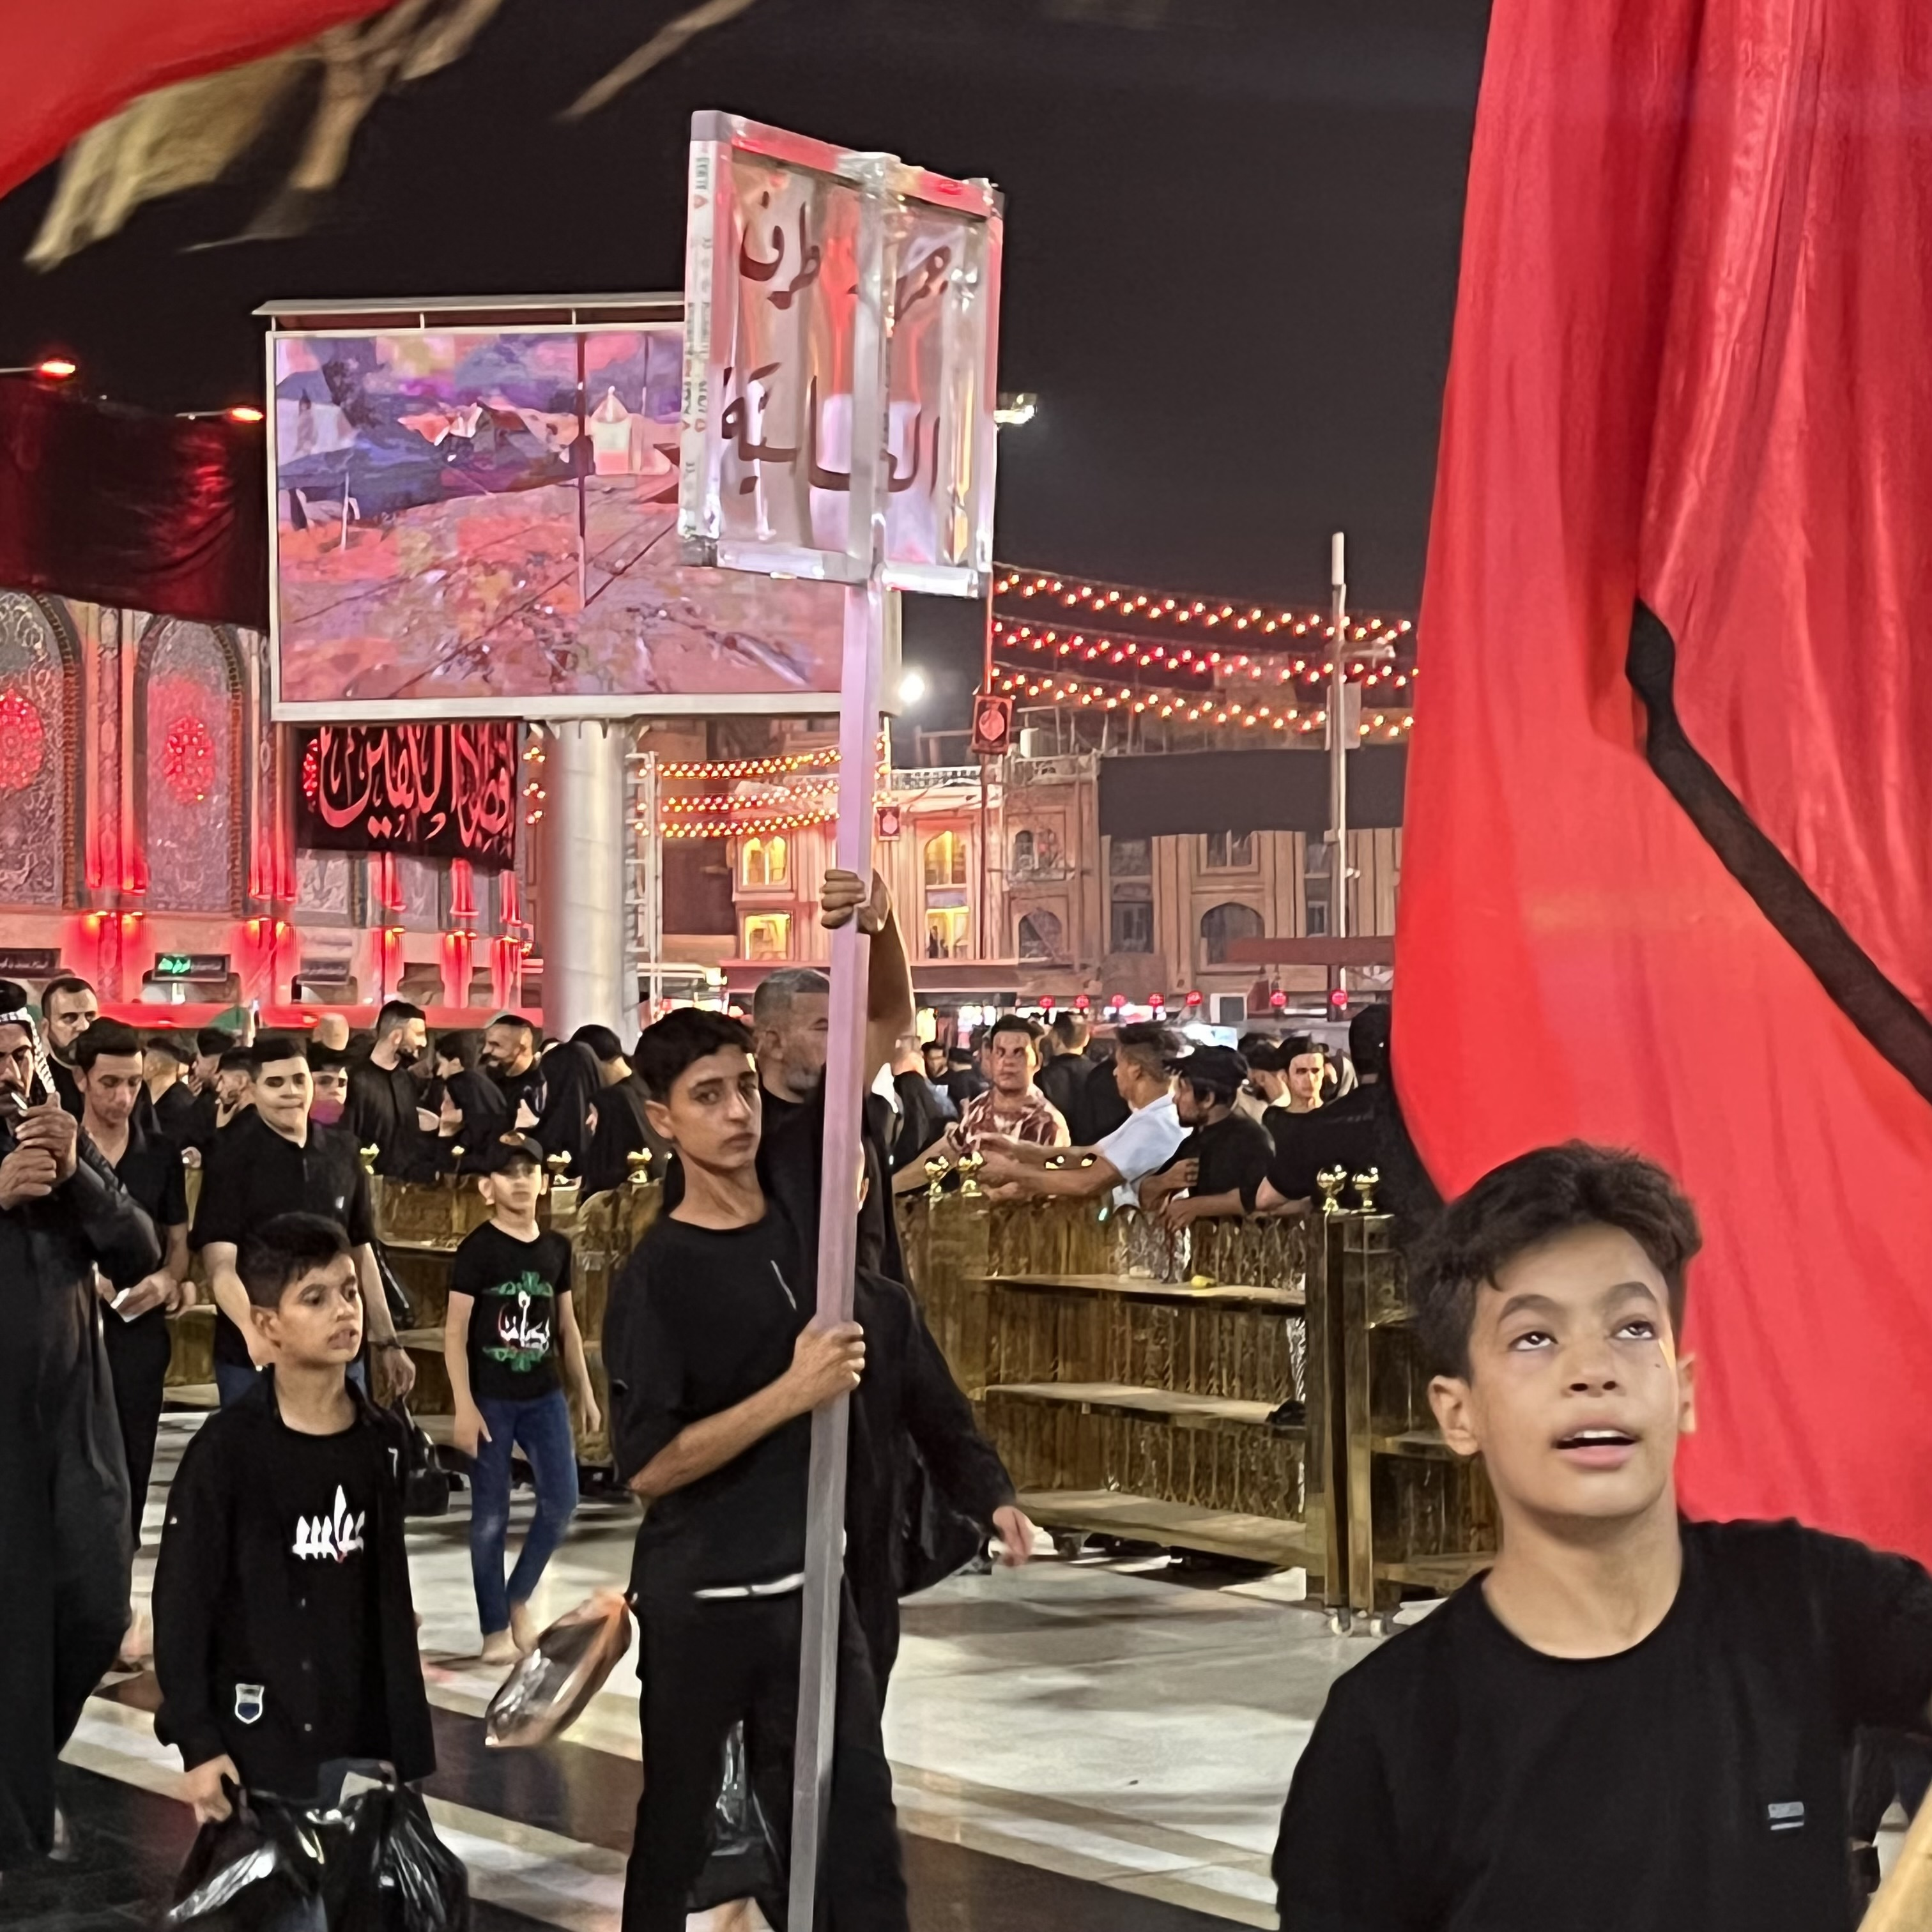
\includegraphics[width=0.4\textwidth]{images/mokweb-abasiyya/bearer.jpeg}\label{fig:radat-bearer}}

  \caption{The various sections of a \emph{radat}. Images taken by author in August 2022.}
\end{figure}

% \begin{figure}
%     \centering
%     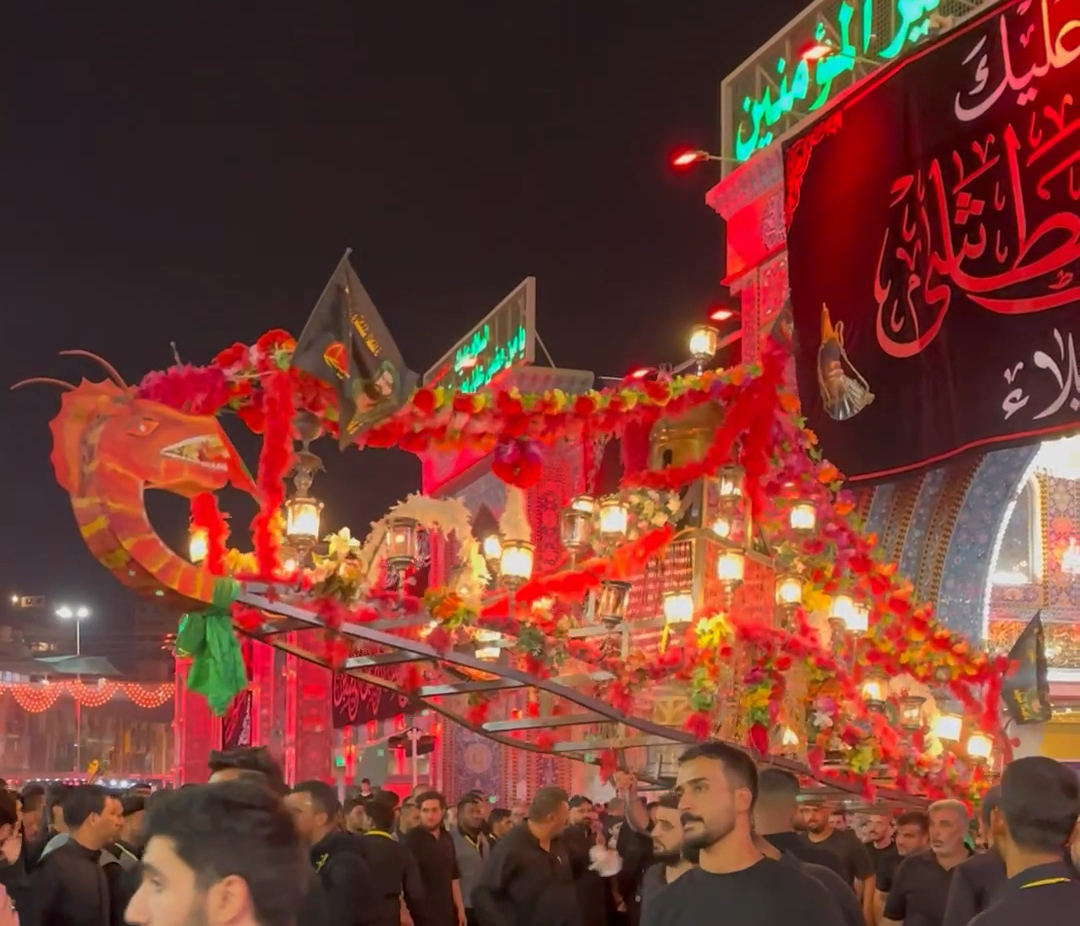
\includegraphics[width=0.5\textwidth]{images/howdej.jpg}
%     \caption{A \emph{howdej} being carried from the shrine of Imam Hussein. Note the snakes emerging from both ends. Image taken by author on August 5th, 2022.}
%     \label{fig:howdej}
% \end{figure}

% \begin{figure}
%     \centering
%     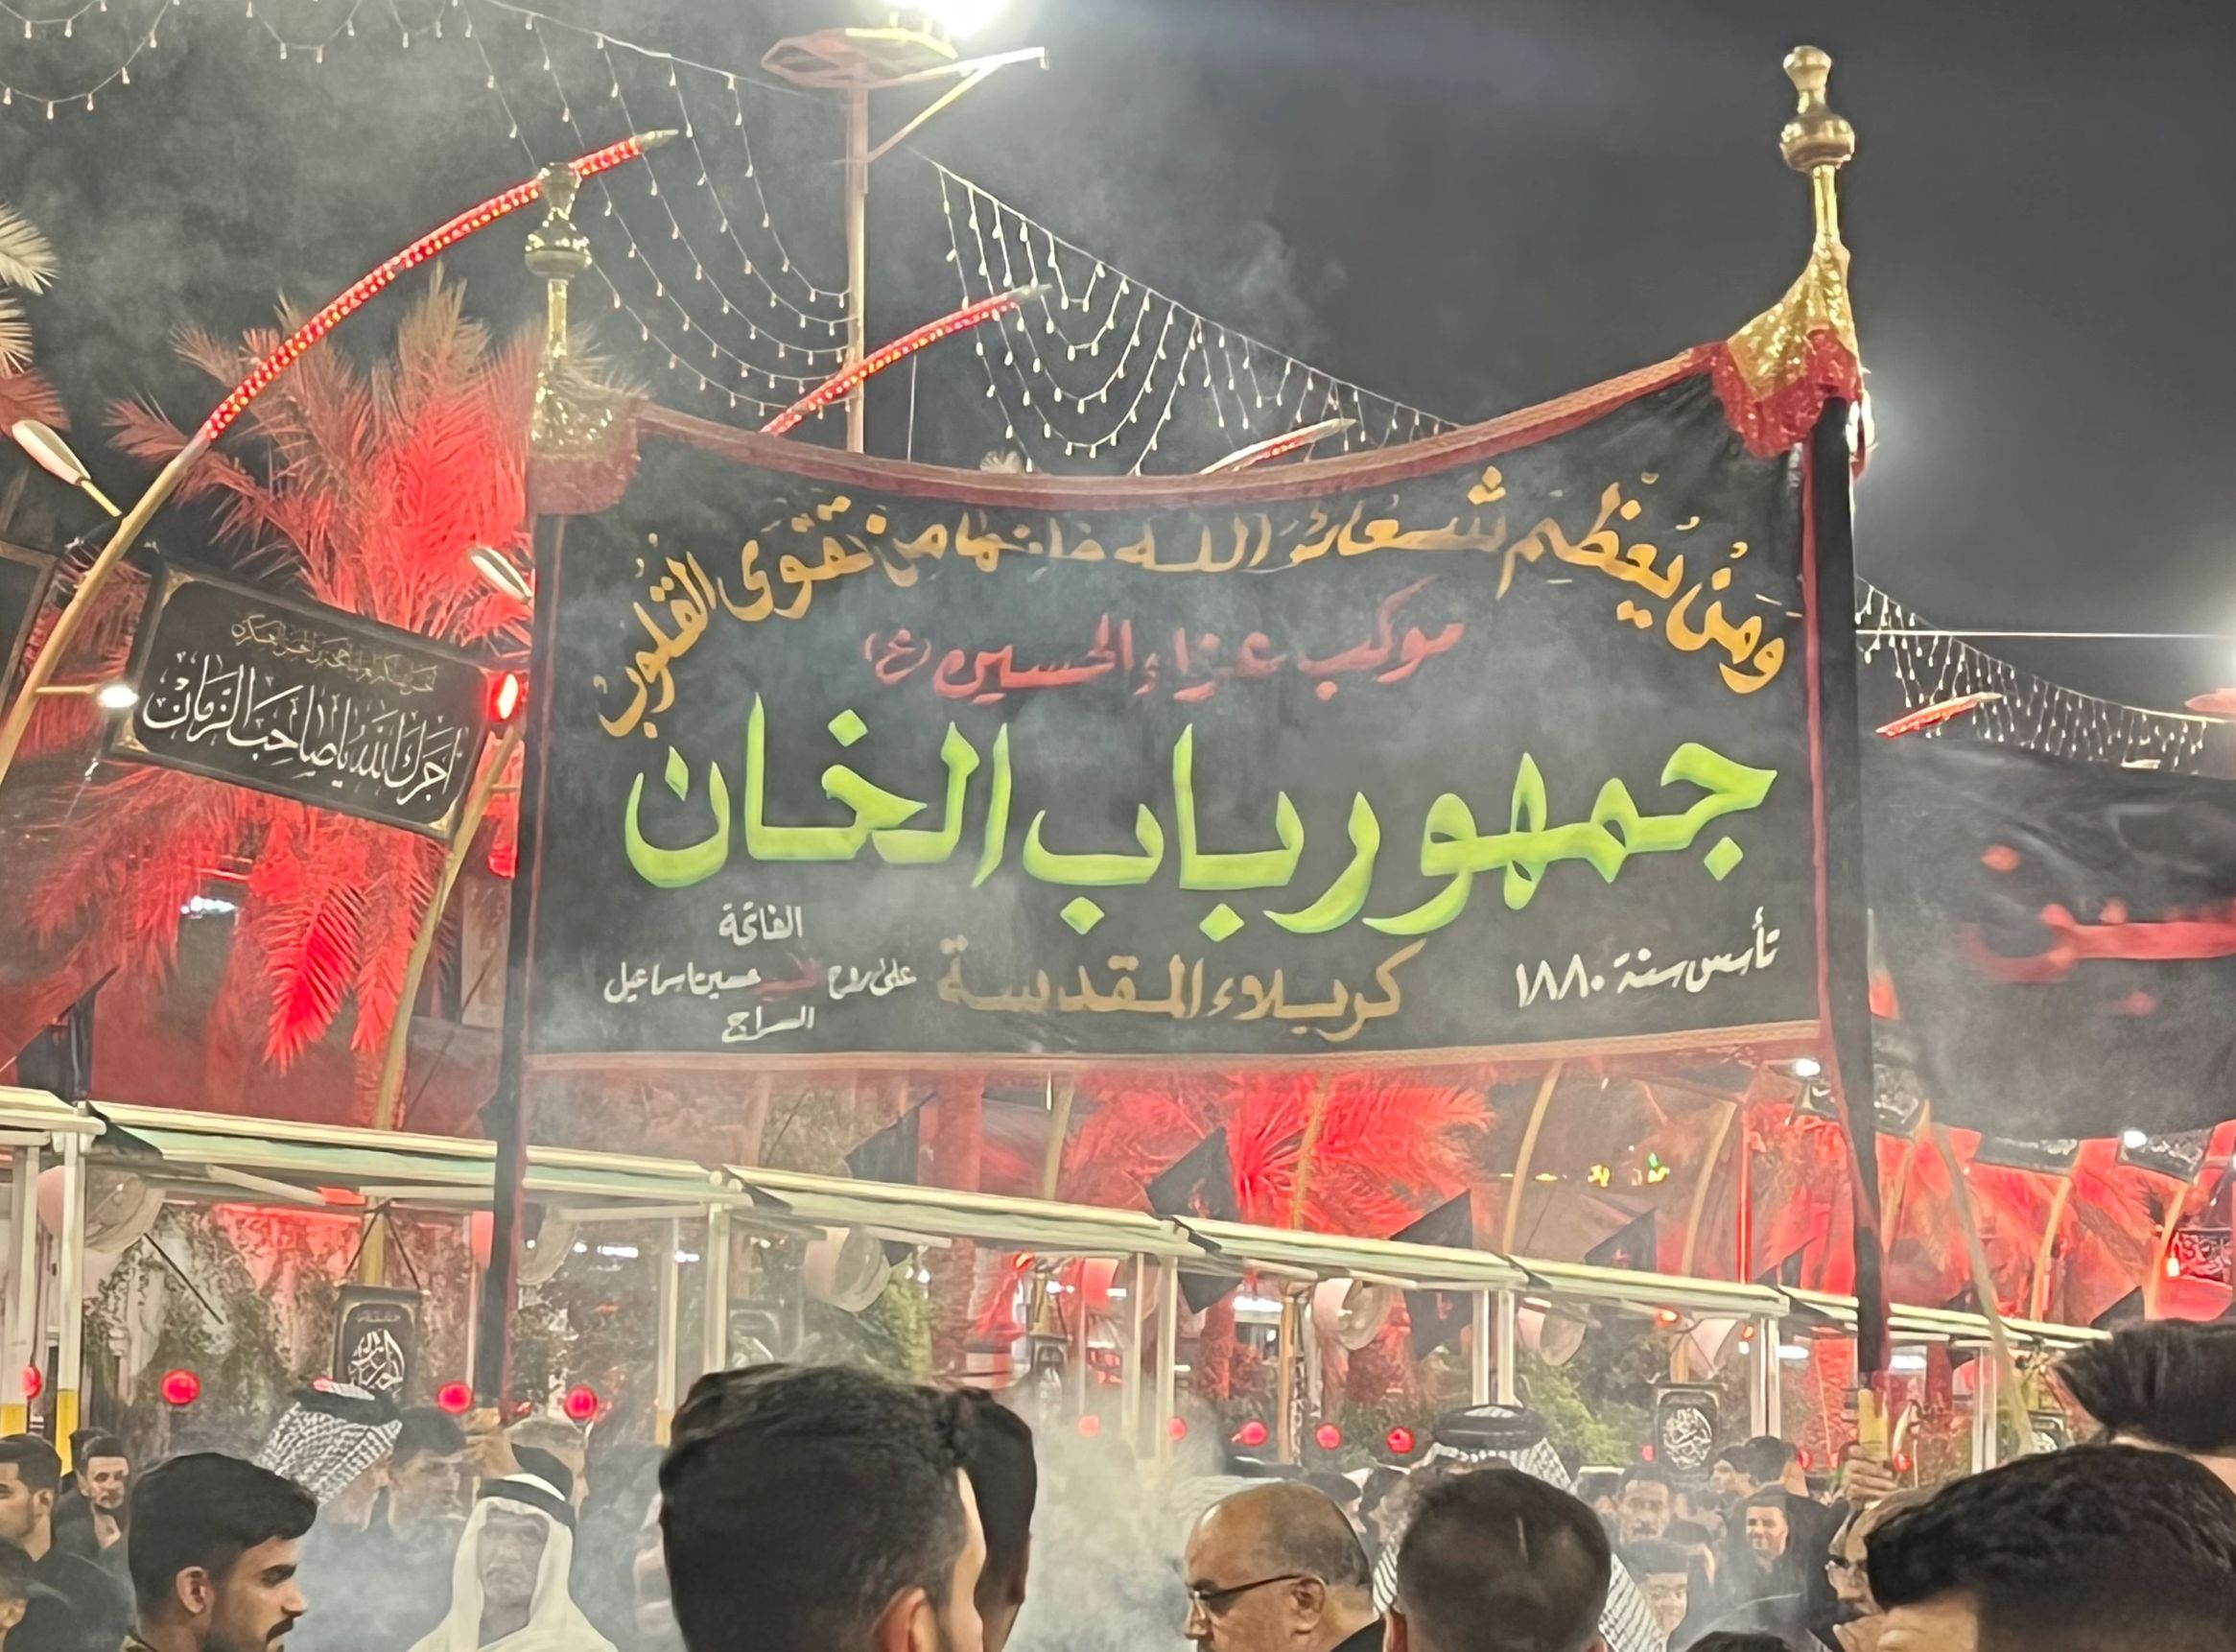
\includegraphics[width=0.5\textwidth]{images/mowkeb-bab-alkhan.jpg}
%     \caption{The banner of \emph{Bab al-Khan} procession. Image taken by author on August 4th, 2022.}
%     \label{fig:bab-alkhan}
% \end{figure}


Following the \emph{howdej} is the main part of the \emph{radat}: the chants themselves. A member of the \emph{mūkeb}, usually a young man, holds a sign and leads a group in chanting. There can be any number of groups, usually ranging from 5 to 10, with each group chanting a section of the poem. Men join and leave groups as they like, but usually due to how crowded the area between the two shrines is, members usually stick with one group, chanting the same three lines and the refrain as they begin at the gate of Abbas, through the Abbas shrine, through \emph{bayn haramayn}, and through the shrine of Imam Hussein. 

Walking with all seven great \emph{muwālkib}, I noticed that the chants were around various different topics. A member of Mukeb Taraf Abbasiyya noted that during previous years, the chants talked about the electricity supply or the water supply in Karbala\footnote{As of 2023, the water supply in all of Iraq is non-potable, and many Karbalaeis do not have access to clean running water. The electricity supply is also similarly problematic, government electricity is only available for 8-12 hours a day, while electricity during the other hours must rely on generator power, which are noisy, polluting, and charge exorbitant rates. As a result, electricity is a constant flash point during summer months, where the government will frequently announce rolling blackouts.}. He went on to describe how all the chants from 2022 were largely centered around Shi'ism or Iraqi nationalism. One \emph{mūkeb} in particular, Mukeb Taraf Abbassiyya, is famously political in their \emph{radat} chants. A section from their 2022 chant reads: 


% \begin{figure}
% \caption{A radat from Mukeb Taraf Abassiyya for Ashura 2022. Image taken by the author, August 2022.}
% \centering
% 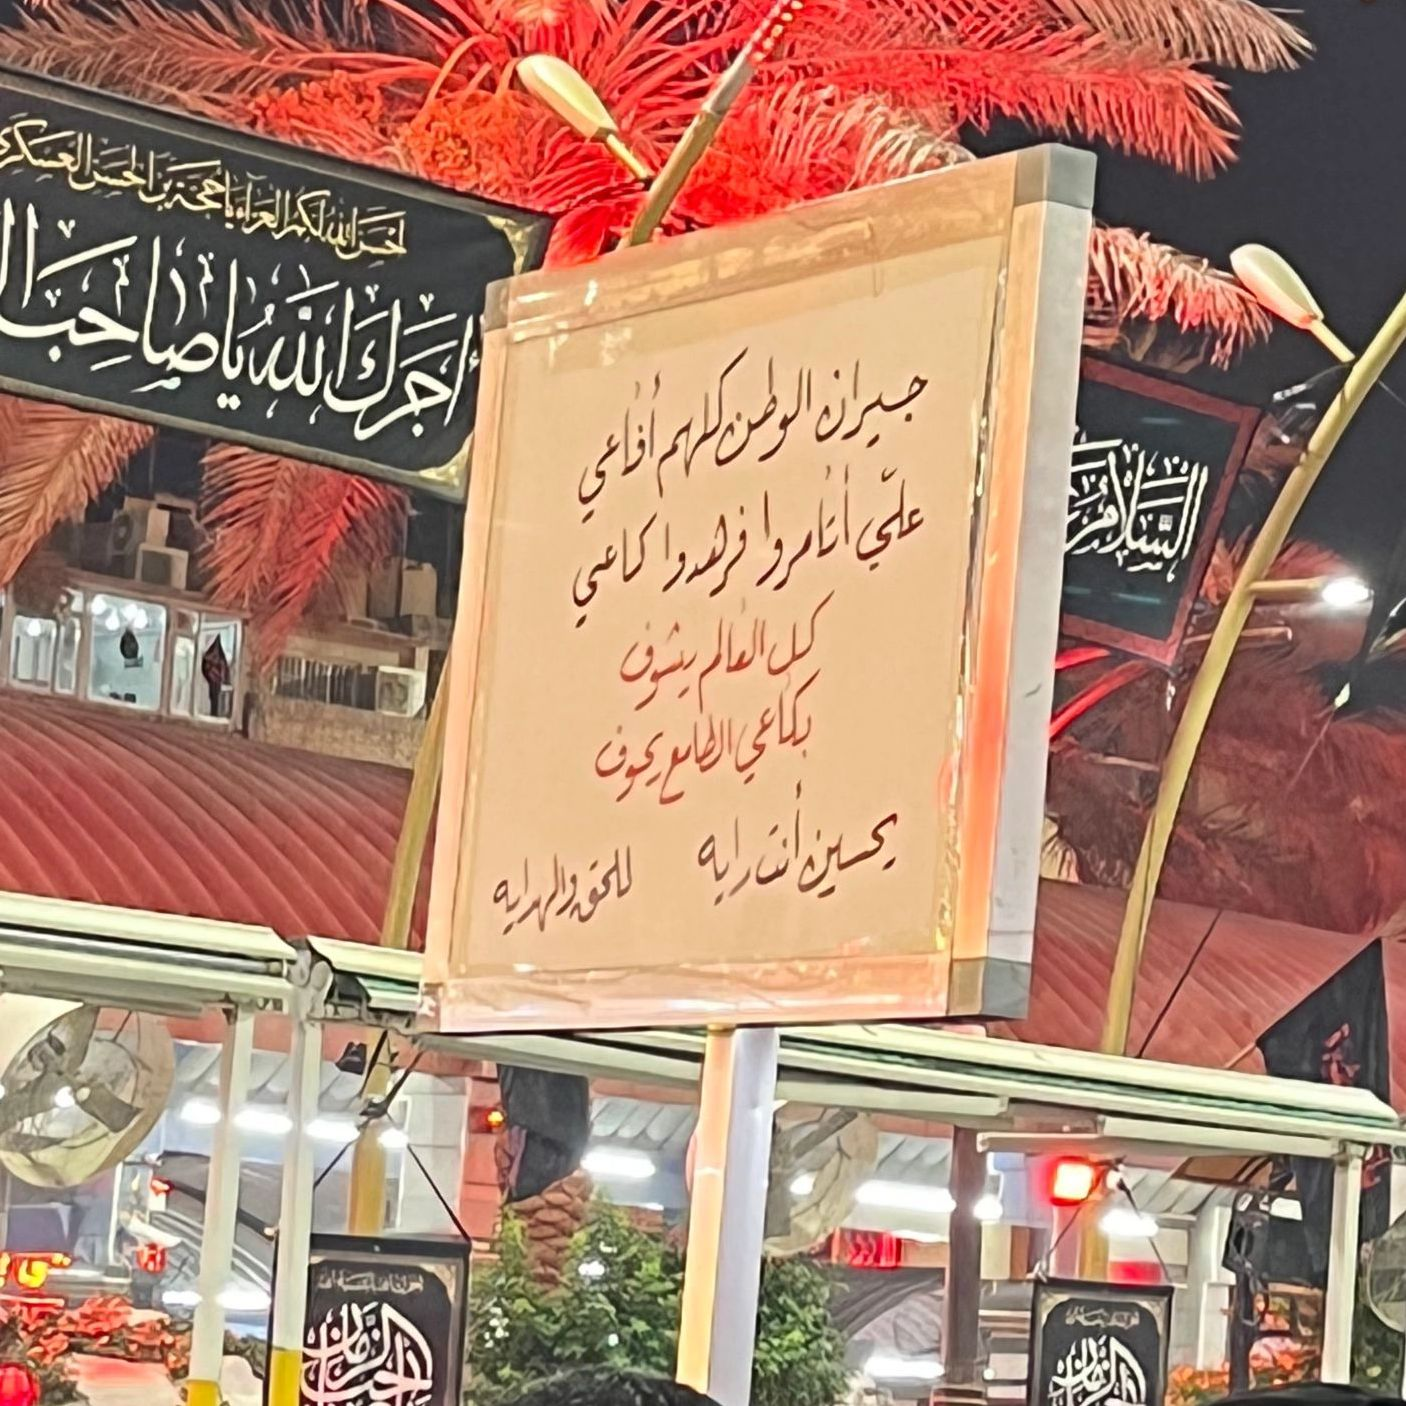
\includegraphics[width=0.5\textwidth]{images/snakes-radat.jpg}
% \label{fig:snakes-radat}
% \end{figure}

% \begin{quote}
% \begin{Arabic}
% جيران الوطن كلهم أفاعي

% علي أتامروا فرهدوا كاعي

% كل العالم يشوف

% بكاعي الطامع يحوف

% يحسين انت رايه

% الحق هداية
% \end{Arabic}
% \end{quote}

\begin{quote}
All of the neighbors of the homeland are snakes

Against me, they conspire to steal my land

The whole world sees

The thieves which roam my land

Oh Hussein you are the banner, the true guide
\end{quote}

On first observation, what stood out the most was the usage of \emph{waṭan}. \emph{Waṭan} colloquially refers to a homeland or nation. Initially, I thought the usage of "\emph{waṭan}" within this \emph{radat} may have referred to an ambiguous Karbalaei conception of \emph{waṭan}, or even a Shi'a \emph{waṭan}, but every person I asked this question refuted this understanding, and stated that \emph{waṭan} refers to Iraq in its modern nation-state form. Taking this, the phrase “neighbors of the homeland” then refers to the current political events occurring between Turkey, Iran, and Iraq. 

This stands in contrast to my interviewees in Baghdad and other cities, who often claimed that the Karbalaei are “Iranians in origin”. When I visited \emph{Wadi Salaam}, the holiest graveyard for Shi'as, two different gravediggers in Najaf mentioned that the Karbalaeis have different politics than Najafis because the area was “settled by Iranians”. 

The paradox between how the Karbalaeis are perceived versus how they see themselves is striking: while they are perceived as foreigners in the state of Iraq, the Karbalaeis themselves see themselves as representative for Iraq, making competing claims to unity. While the usage of the Iraqi flag during rituals may be seen in a sectarian light, such as Shi'as laying claim to the state and the nation, the \emph{radat} provides additional depth. By claiming the neighbors of the \emph{waṭan} are snakes, the Karbaleis are carving a different path beyond simple sectarianism, they are making a claim to a particular form of unity that incorporates that deeply incorporates the conceptions of the nation-state, in contrast to the ideas about the "Shi'a crescent" \cite[120]{haddad_understanding_2020}. 

The \emph{radat} chants also present themselves as an interesting intersection of the political, the religious, and class. Rather than seeing these spheres as disparate spheres, the Karbalaei themselves easily mix these together, with the conceptions of the nation-state interacting with the fact that the ‘ulema do not participate in these chants. There is a special \emph{mūkeb} called Mukeb Imam Hussein which is affiliated with the workers and members of the Shrine of Imam Hussein, but this \emph{mūkeb} is not affiliated with any traditional neighborhood. The overriding notion is not politics or sectarianism, but rather a distinction within the religion between the language, between the religious educated and the rituals of the streets. What is more interesting is that the \emph{radat} chants are a purely oral tradition, upon asking various historians and poets affiliated with different \emph{muwālkib} and the shrines, the tradition is strictly oral. The \emph{radat}s conducted by the Karbalaeis are avowedly present in nature and similar to majlis: the chants are about current events, or past events drawn into the present, while their oral nature allows them significant room to change: the past is malleable because it is not conducted in MSA, and conducted in the tongue of the people. 

In contrast, Najaf has held a so-called quietist tradition, rooted in a disdain on the part of Shi'a jurists towards involvement in politics and daily political activities \cite[216]{hamdan_development_2012}. This quietist tradition has paradoxically led to a mystification by scholars on the conditions in which Najafi clerics do become involved, such as the case of the "Najaf Veto" described at the beginning of the chapter. 

The oral nature of \emph{radat} and the rooting of \emph{radat} in distinctive neighborhood identities has enabled Karbalaeis to articulate their grievances and political positions. Cross-cutting politics, religion, and class, the \emph{radat} of previous years focusing on electricity and water functions as an act of resistance against an incompetent and corrupt government. The \emph{radat} of 2022, when clamoring for a specific Iraqi \emph{waṭan}, shows how the same ritual can be repurposed to mean a specific version of unity. Similarly to how the Salafi women in Saba Mahmood's work played an active role by shaping their own senses of conduct by breaking customary norms \cite[87]{mahmood_politics_2005}, the Karbalaeis break from the Najaf quietist tradition.
% \section{\emph{Tatbir}}
% Ashura, the 10th of Muharram, begins at dawn. I had slept at a \emph{husseiniyya} near the Shrine of Imam Hussein the night before in order to witness the event in its entirety. The \emph{husseiniyya} was already packed with pilgrims when I arrived the night before, I found a small cot near the wall and napped for a few hours. At 3:30am, I stumbled over to the Qibla road, the road that terminates at Bab al-Qibla in the shrine Imam Hussein. When I arrived, the celebrations were already in full swing. A throng crowded the streets, with soldiers and policemen attempting to divert the sea while maintaining distance from the people. The main event was about to begin, with the focus on \emph{tatbir}. 

% \emph{Tatbir} is the practice of ritualized bloodletting. Shaving of the head, followed by cutting of the flesh, either through quick, repeated strikes or a swift incision on the surface of the skin is made. \emph{Tatbir} is religiously controversial, even among the Shi'a, Ali Khamenei forbids \emph{tatbir}, Ayatolla Sistani has never given a fatwa on it, and other opinions of the clerics range from completely forbidding it, to allowing it under special circumstances, to encouraging it as a mustahab act. The Iraqi Shi'i \emph{mutjahid} ‘Abd al-Husayn al-Hilli has argued that the formation of these \emph{tatbir} and other ritual lamentations have become public events in recent years, but notably only mentions weeping and beating of the chest as religious obligations \cite[85]{weiss_shadow_2010}, with \emph{tatbir} conspicuously absent from his rulings. Theological debates aside, the International Media Department of the Shrine of Imam Hussein attempted to bar me from taking photos of \emph{tatbir} in previous discussions, although such a rule was impossible for them to enforce. 

% Dressed in white to showcase their bleeding, I saw a massive crowd march towards the gate of Imam Hussein, all men of various ages. I saw a young boy with a shaved head, no more than ten years old, walk up to an elder, offering the older man a small kitchen knife. The elder man made a swift and precise incision at the base of the skull, drawing blood, and offered the boy a white cloth to gather the blood. Other men held large swords, repeatedly vertically striking themselves on their skull with repeated shouts of "Haider!", another name for Imam Ali. From the second floor of the shrine, I could see women pressed against the window, watching the men. Cottons swabs soaked in iodine were handed out from various volunteers to sterilize the \emph{tatbir} wounds. A shocking amount of blood flowed in the streets with the mass of people making it impossible to move freely. Pushed around by the crowd, my sandals became stained in blood. Other spectators pressed their kuffiya or their shirts against their face to prevent themselves from vomiting. The air reeked of blood, iodine, and sweat. 

% As the crowd pushed me towards Qibla gate, I saw the participants cry out and raise their blades towards the sky. Drums and trumpets blaring, they marched into the shrine as I ducked out from under some swords.

% Like \emph{radat}, \emph{muwālkib} arrive in procession to perform, although instead of black banners, the \emph{tatbir} ones utilize white banners and red text, mimicking blood, playing a similar role to \emph{radat}s. However, the key difference is the hemic element, cutting of the head and bleeding is meant to evoke an imagery of sacrifice and justice. Edith Szanto has written about \emph{tatbir} in the context of the Damascus, noting how women were particularly proud of their husbands for participating \cite[86]{szanto_beyond_2013}. In a similar way, \emph{tatbir} in Karbala provides the same: I witnessed a young boy, no more than 8, having his head cut open by an elder. Afterwards, the entire \emph{mūkeb} gathered and congratulated the boy for his first \emph{tatbir} experience. The \emph{tatbir} experience a literal sublimation of the self via blood which then binds people together\footnote{Blood brother style rituals are similar to \emph{tatbir}. In Iraq, another tribal practice is called Kriev, which is similar to a blood brother ritual, but serves to bind two families. Kriev is a circumcision ritual, a boy of a weaker family is circumcised in the lap of the patriarch of another, more locally powerful family. Krievs were conducted between Yazidi families and Arab families before ISIS, however, many Yazidis have turned against the process, as many were given up to ISIS when they sought protection from their kriev families. It is unclear to me where the origins of the Kriev are, I have interviewed non-Yazidi Kurds with Kriev families all over northern Iraq. The practice seems less common in the south, however.}. 

% \section{Services}
% The most visible role of \emph{muwālkib} for pilgrims is during Ashura and Arbaeen, where \emph{muwālkib} provide services such as food, water, and places to rest. \emph{Muwālkib} will setup tents, with the numbers ranging from one to many, offering a dizzying array of services, such as medical care, bathrooms, foot massages, cooked food, areas for rituals, and so on. Other \emph{muwālkib} offer memorial services, such as many Hashd \emph{muwālkib} providing a museum for viewing propaganda as well as museums of war memorabilia for fallen martyrs of the Hashd. During Arbaeen, I walked through a \emph{mūkeb} which featured a cardboard cutout of both Qassem Soleimani and Abu Mahdi Muhandis, two men who were killed by the United States in early 2021. As both men were key figures in the militia regime between the Hashd al-Shaabi and the Iranian Republican Guard Corps, this \emph{mūkeb} offered a chance for pilgrims to see mock graves and take photos with their respective uniforms. 

% Iraqis residents raise money throughout the year in order to provide these services, including soliciting donations from the local community and around the world if they have additional resources. With innumerable service \emph{muwālkib} during every ziyara, an immense amount of resources is poured in, from furniture to cleanup to raw food material.

% Many of my interviewees pointed out the inclusive nature of service \emph{muwālkib}, with service \emph{muwālkib} being run by Lebanese, Iranians, Bahranis, and so on. The walk between Najaf and Karbala is approximately 80 kilometers, and the unit of measurement is electrical poles, which span every 50 meters. Pilgrims during the walk refer to specific \emph{muwālkib} near different poles as identification. Near pole 596, I saw a \emph{mūkeb} being run by Thailand Shi'a, who had a large banner written in Thai mentioning that it was the eighth time this group of Thailand Shi'a had done this. 

% Lale Can has written about the Sufi culture of guest lodges for pilgrims, which provided similar services and served as institutions of learning for Sufi pilgrims travelling to Mecca and Medina \cite{can_spiritual_2020}. Can noted that these lodges existed in precarious positions with regard to the Ottoman state authorities that managed pilgrimage, with fears from state authorities that pilgrims would overstay their welcome by living the the guesthouses for an extended period of time. The tension between the Ottoman Empire's role as a Muslim empire competed against the state imperative of control of guests via passports. As Christopher Low describes, the Ottoman Empire was deeply concerned about the rise of Indian immigrants to Mecca and Medina and how the empire authorities saw them as British subjects, and therefore a play by the British to assert control over the Hijaz \cite{low_imperial_2020}. 

% These tensions of state needs and religious needs continue today, albeit in slight different forms. The key difference in that Sufi guest lodges usually were attached to a specific mosque or waqf. Shi'a \emph{muwālkib} can be affiliated with any group, whether that group is a specific militia, homes or group of homes, or even individuals. Inside city limits of Karbala, especially closer to the shrines, \emph{muwālkib} require a license, which are issued through the al-Kafeel Department of \emph{Muwālkib} near the Abbas shrine. However, outside city limits, especially on the road from Najaf to Karbala or Baghdad to Karbala, \emph{muwālkib} are effectively unregulated, anyone can place a \emph{mūkeb}, start \emph{mūkeb}, collect donations for one, and so on. 

% The sheer number of \emph{muwālkib} only complicates the relationship they have with the state. The Iraqi visa regime is complex and often confusing. A brief discussion with the Thailand Shi'a revealed that the religious visa, which is intended to offer 30 day stays for pilgrims, is often not enough time to sufficiently prepare, such as organizing logistics around food, electricity, and generators. As Muharram has shifted into the summer months, air conditioning in \emph{muwālkib} has become a necessity, despite the fact that the electrical grid continues to deteriorate whenever summer arrives in Iraq. Karbalaeis mentioned on multiple occasions of the negative view towards Iranians, specifically the stereotype of Iranians as freeloaders who come to Iraq only to demand free food and lodging, while throwing trash everywhere and providing nothing in return. 

% One key point that was repeated is that the Iranian pilgrims arrive in Iraq without a passport. During normal conditions in Iraq, there are checkpoints between every governorate, as well as within Baghdad itself, and before specially closed areas. Iraqis and foreigners grow accustomed to these checkpoints, with the checkpoint police often being the butt of jokes as uneducated and illiterate. In addition, these checkpoints are not only run by the state, they are run by a variety of militias and local groups. For example, the checkpoint into the city of Samarra is run by Sayara Salaam, or Peace Bridages, the successor militia to Muqtada Sadr's infamous Jayesh al-Mahdi, while a checkpoint on the Jadriyah bridge in Baghdad, one of the major arteries of the city, is run by the Kurds. The formal legislation around checkpoints seems loose as well, crossing into different cities often requires two or three checkpoints, usually with a state checkpoint followed by one or two militia checkpoints. While these checkpoints have become routine to people's lives, they are also very serious, checkpoint police have unilateral power to arrest and detain anyone for an indefinite amount of time. For example, when attempting to cross into Samarra for the first time in 2021, I was arrested by the checkpoint police for "seeming suspicious" and thrown in jail for over 18 hours with other men who had been detained, some of whom had been in jail for months. The high stakes nature makes it such that every foreigner in Iraq, and even Iraqis, know that proper documentation is necessary, lack of proper documentation could result in major consequences. 

% However, during Arbaeen, most Iranians arrive without a passport, crossing the Iran-Iraq border with only their Iranian ID's, and often without any money as well. The checkpoint between Najaf and Karbala is typically an array of concrete walls manned with soldiers, yet during Arbaeen I was shocked that it was completely unmanned. Pilgrims simply streamed through the checkpoint, and the only process resembling the feared bureaucracy was a simple, hurried patdown. The scale of pilgrims, and the sheer amount of services and lodging available from service \emph{muwālkib} meant that there was always more capacity for pilgrims, inducing demand. This overwhelmed state capacity, to the point where the state must partner with independent organs like the Hashd, who blare out propaganda images and videos of Hashd soldiers guarding the road. 

% - talk about the thai \emph{mūkeb} and international \emph{muwālkib}
% - talk about the perception of generosity and the role that \emph{muwālkib} play
% - raising chickens in the backyard and fattening them, the role of \emph{muwālkib} matter a lot for individual residents 
% - talk about the perceptions of Iranians 

% \section{Hosa}
% Hosa is a tribal ritual conducted by south Iraqis. Hosa consists of two to four people, engaged in verbal poetry. Similar to slam poetry or battle rap, hosa is rooted in tribal tradition. Spectators organize in a circle around the participants performing hosa, and draw a wide audience. A rural/urban split occurs as well, as urban south Iraqis do not perform hosa. 

% I first encountered hosa during the nights leading up to Arbaeen, where I saw it being performed in the streets around the shrine of Imam Hussein. After asking a few people, they described hosa as a tribal ritual, and not a necessarily Shi'a one. Hosing provided an interesting mix of local cultural traditions mixing with religious traditions: pilgrims, who had come to Karbala in order to perform visitations had brought their own rituals as well. This matches to the descriptions my interviewees had about various forms of latm from other non-Arab Shi'as: \emph{latmiyyat} from Pakistani Shi'as were described to be more violent, while \emph{latmiyyat} from Iranians were perceived to be quicker in pace. 

% \section{Repetition in the Procession}
% A key part of both rituals is iteration: both rituals draw in the participant and revolve around repetition. Hamid Dabashi has written about an Iranian Shi'a ritual called \emph{ta'ziyah}, a play similar to the Christian Passion plays. He specifically describes \emph{ta'ziyah} and Shi'ism as a constant mourning: "the act of remembrance will have to remain always incomplete-like a dream that keeps haunting a people, forcing them to try to remember it, but never successfully." \cite{dabashi_taziyeh_2005}. Repetition here serves as the basis for a certain type of harmonization between people, either in lieu of possession, or in some cases, actual possession. Through repeated chants, participants internalize specific states, either with the concept of tragedy or mourning. Through repeated symbols, each repetition moves recognizes the previous one, but adds new features. The \emph{mūkeb} procession is a key example of this.

% As mentioned before, the \emph{howdej} is a heavy boat that begins every \emph{mūkeb} procession. Derived from the word \emph{howdej} in Arabic, meaning a bed carried by a camel, the \emph{howdej} is usually carried by one or two men during a procession. Shaped like a triangle, the \emph{howdej} is richly adorned with lamps and flags. The core of the \emph{howdej} is a metal pyramid structure, often bearing remarks related to Hussein. Lamps are placed symmetrically on each side of the pyramid, with a single lamp at the very top. There is significant variation in \emph{howdej}, with only the core structure being regulated. 

% \emph{Howdej}, at the beginning, lacked the snake-like creatures that represented the coming evil against Imam Hussein. When asked, many residents of Karbala could not tell me when this feature as added, but recognized its symbolism. Latm and qasidas have similarly incorporated drums and other features throughout time, but retain their clear identity. The rituals have also taken on a showmanship identity, with individuals competing against one another, such as in the case of carrying the pillar on the head. 

% Recognition is even more explicit, because of the overly public nature of the rituals. Building on that the rituals are recognized as \emph{husseiniyya} rituals, the public spectacle element of the rituals means that iteration happens faster than before, leading to new additions and changes. Another example of this is the flag changing ritual, where the flags are pulled down and changed before Muharram. This ritual began in 2006 \cite{hamdan_development_2012}, and is extremely conspicuous, as the flag and domes of Karbala are omnipresent in the imagery. 

% It is impossible to attend a majlis or \emph{radat} that is not photographed, videotaped, or livestreamed in Karbala. The holy nature of the city means that visitors are encouraged to videotape, but because rituals participants recognize themselves and others within the photograph, they are encouraged to compete and iterate, not only with their peers, but with their past selves. The photograph, as Johnson states: "mediates a scene or person in a place and time different from those in which the photograph is viewed and the here and now. The quality of being at once an image and a thing is important because it enables the photographs’ multiple lives, crossing dimensions" \cite[92]{johnson_automatic_2020}. Photographs and videos are not a side-effect on the ritual, which pushes it forward, but rather a part of the ritual itself. In the same way the latm draws in the participant by encouraging them to chant, \emph{husseiniyya} rituals in general encourage participation through videotaping. The rituals are not spectacles that get photographed, they are spectacles because in order to encourage photography. 

% \section{Photography and Language}
% One curious practice I saw was bringing people virtually to Karbala by dialing a video call or pulling up a photograph, placing the person’s image upon the background of the shrine, and using a second phone to take a photo. I saw men using a Whatsapp video call, then placing their mother’s face in the phone against the backdrop of Bab al-Qibla of the Shrine of Imam Hussein. Similar photographs abound on social media, where they are endlessly reposted \footnote{https://twitter.com/JawadAbubakar7/status/1570739286873612290}. Similar to the explicit rituals, the end result of this is a photograph of a person and the shrine, showing that the photograph generation holds the key here. 

% During a casual conversation with my neighbor, he mentioned how the \emph{howdej} had changed very quickly within the last few years, including sprouting snakes at each end of the boat. Marching with \emph{howdej} is also a very public ritual, ritual participants are eager to show that they can carry a \emph{howdej} by themselves. Cries of "mashallah" surround the bearer as they are recorded, shared, and re-shared along social media. 

% Combined with the common practice of carrying around two smartphones in Iraq\footnote{This is due to various issues with cellular service, oftentimes Iraqis have a single smartphone for internet service, and another for calling, as they are billed separately. Internet calling via WhatsApp is significantly more expensive than minutes.}, photography and videotaping of Karbala is central to the formation of the city itself. The affordability and ease of photo and video sharing, especially driven through the overwhelming popularity of Instagram within Iraq, infuses social networks with religious motifs. Rather than merely hearing stories about the veneration of the sacrifice, pilgrims see and hear the city before they come, familiarizing themselves with site itself. Karbala itself fractures: the Karbala of photography and videos, the Karbala of the stories and hadith, and Karbala the city in reality.

% Photography, as an act, is also a temporal one. As Johnson mentions, "a photograph mediates a scene or person in a place and time different from those in which the photograph is viewed and the here and now." \cite[92]{johnson_automatic_2020}. Johnson identifies how photographs cross spatio-temporal lines by first drawing in the photograph's maker in relation to the site and subject, and second by imprinting the imagery upon the viewers. \cite[92]{johnson_automatic_2020}. 

% The secondary effect of the outpouring of photographs and videos is the iteration of rituals. Many of my interlocutors, both of the clerical class and laity, mentioned how the rituals have changed at a faster rate within recent decades, becoming more and more dramatic. In the economy for attention, ritual performers now must not only compete with just the other ritual performers around them, but also the ritual performers of the past, who are eternalized within photographs and videos. This game of one-upsmanship has accelerated the rate of change, I saw young men attempting to show off to their groups of friends how they could carry the \emph{howdej}, displaying their strength and skill. 

% Karbala is experienced not through just physical existence, even present pilgrims experience the self mediated through the apparatus of photography. This environment is nearly surveillance like, one cannot escape being in a photograph or video and ending up on social media. The result of this environment is people who feel at ease with it, performative actions seep in without conscious thought. The ritual sites are almost tailored for photography and video: dramatic photos of shirtless men beating their chest, bright flowers and signs adoring every corner, entire houses drenched in blood red lights for liturgical performance. Pilgrims bear flags of their \emph{mūkeb}, their militias, and their countries to be sanctified. Through both showing photos of friends and family as if they were physically present in Karbala, or through consumption of ritual imagery, photographic and videographic records prove to pilgrims that they were present within the holy city, while promising community and faith to future pilgrims. The city bridges modern day Shi'a to the their temporally estranged Imam, but the truth is that the acts of repetitive performance create Karbala's future. Time, through the city's connection with past sacrifice of Hussein to the promise of potential future rituals, becomes integral to the city and the religious experience. 

% Curiously, another story about Karbala has become popular just as photography has taken off: the story about the smell of apples \cite{sayyid_rasood_interview_2022}. Within Shi'a hadith, Imam Hussein is said to have stated that, while his troops were thirsty in the desert, to imagine the taste of apple, and quench their thirst as a result. A common belief is that, upon entering Karbala with a pure heart, a pure pilgrim may smell apples. This myth, while appearing to be yet another myth of visions or belief, is interesting because it makes for what photographs are not: the sense of smell. The holy city’s values are sensorial: all senses are activated in the recognition of ritual.

% The role of the city seen as a ritual site means that both pilgrims and residents draw upon it. In one instance, when I had a mysterious cold during my fieldwork, I jokingly asked my friend Abu Shams if it was appropriate to go to Hussein and ask him to cure my cold. In response, Abu Shams told me that the cold was a trivial matter, but elaborated that people go to the Tomb of Hussein in order to cure major illnesses, and people go to Abbas in order to ask for vengeance when they have been wronged. 

% The suggestion of an internalized ranking of what one should ask saints is common in hagiography, as colds are deemed too trivial, but cancer is serious enough, The closeness of the saints through ritual is compared to the distance of photography, both evoking a new form of strangeness. Pilgrimage is not necessarily the key here, but rather the generation of photography is. 

% As mentioned before, another key distinction between the Shi'a rituals and the Sunni ones, such as Khutba, is that the Shi'a rituals are all conducted in the vernacular. Similar to the Vatican II accords, where it was decided in 1956 that liturgies should no longer be conducted in Latin but rather in the local vernacular to allow participants to become closer to their religion, Shi'a rituals perform much of the same way. Mustafa Soufan argues that the split of language in Arabic between Modern Standard Arabic and colloquial has estranged the government from the people \cite{safouan_why_2007}. 

% The functional explanation of this for Shi'a rituals is that Shi'a’s, as the religious minority within Islam, cannot afford to alienate themselves. While this might be true, it could also be argued that using Iraqi Arabic, as opposed to MSA, actually casts Shi'as in a negative light. The sectarian overtones of everything in Iraq suffuses this, amplifying the desire to perform acts of distinction. 

%Ali al-Wardi cited a process within Iraqi cities that he titled "ruralization" of Iraqi cities, stating that, contrary to popular belief that rural villagers become more liberal and cosmopolitan as they move into cities, Arab cities tended to follow a pattern that followed the opposite: cities became reshaped along rural lines, reinforcing their tribal and clan boundaries.

% \emph{Muwālkib}, as temporary and dynamic congregations, are a testament to the power of community in shaping Shi'a identity. The \emph{muwālkib}' role in the commemoration of Imam Hussein's martyrdom during the annual Arbaeen pilgrimage transcends the traditional boundaries of religious hierarchy. This decentralized organization, united by a common purpose, nurtures a sense of belonging and shared values that enrich the Shi'a experience.

% This repetition not only strengthens the emotional connection of participants to the rituals but also promotes a sense of unity and belonging within the community. At the same time, the inherent dynamism of oral traditions allows for variation, adaptation, and reinterpretation, providing the opportunity for open-ended change within the Shi'a faith.

% Moreover, the performative nature of \emph{radat} chants and other rituals emphasizes the collective experience and shared cultural heritage among adherents. By engaging in these practices, individuals contribute to the perpetuation and evolution of their religious and cultural identity. The flexibility of these oral traditions enables them to act as a living repository of memory, values, and beliefs, responding to the needs of the community and fostering an environment for continual growth and change.

% \subsubsection{\emph{Tatbir} Controversies}
% Sayyid Muhsin al-Amin al-Amili (d. 1952) was the highest-ranked jurist in Damascus in the 1920's when he published a tract condemning bloody acts of self flagellation \cite{ende_flagellations_1978}, \cite{szanto_beyond_2013}, \cite{weiss_shadow_2010}. This proceeded to set off a firestorm of debate, which Werner Ende referred to as "the great Shi'a \textit{fitna}" and what Max Weiss calls "The Ashura Debates". Born in 1867/1868 and after acquiring his marjia' status from Najaf, al-Amin proceeded to publish a five-part work called al-majalis al-saniya \cite{ende_flagellations_1978}, \cite{weiss_shadow_2010}. Notably, this work suggested "purging unsound sources or inaccurate accounts, proscribing certain practices as well as calling for a deeper awareness not only among Shi‘i ‘ulama’, but also among lay believers, of the social and political ramifications of engaging in such cultural practices in the first place" \cite[76]{weiss_shadow_2010}. 
% The interest in the preservation of the image of Shi'ism by al-Amin by reforming a specific subset of practices hints at the priorities at stake. Why was \textit{\emph{tatbir}} considered worse to the image of Shi'ism than elegies? Why is crying to niyahah considered just as bad for the image of Shi'ism as \textit{latm}iya listening to a \textit{radood}? Notably, al-Amin was not the only one at the time who attempted to reform certain practices, Werner Ende finds that Sayyid Abu l-Hasan al-Isfahani (d. 1946), the supreme mujtahid of Najaf at the time, and Sayyid Muhammad Mahdi al-Qazini (d. 1939), another prominent Iraqi Shi'a cleric based in Basra, both issued fatawa attempting to exclude what they saw as wrong and harmful practices \cite[72]{hamdan_development_2012} \cite[26]{ende_flagellations_1978}. Weiss attributes this fear of poor image to others as a modern sense of the sanctity of the individual body \cite[80]{weiss_shadow_2010}, finding that al-Amin hides a universalistic impulse: the human body is sanctified, either as Shi'i or non-Shi'i, and an "an attempt to render “traditional” religion palatable to a newly envisioned Shi‘i public, to effectively modernize tradition in the process." \cite[81]{weiss_shadow_2010}

% While Weiss's reading of the body in al-Amin seems to be a factor, the more overt factor seems to be that making the rituals palatable provides a greater chance of a conversion. In addition, 'Abd al-Husayn al-Hilli, another Iraqi \textit{mujtahid} buckets \textit{\emph{tatbir}}, \textit{latmiya}, and weeping all into the same bucket \cite[85]{weiss_shadow_2010}. Weeping, as a ritual tool, should have seemingly no violation of the individual sanctity of the body, and in fact, weeping for Hussein was declared as "I am the martyr of tears (\textit{qatil al-ibrah}), no man of faith remembers but that he weeps" \cite[143]{ayoub_redemptive_1978}.

% What appears to be at stake here is palatability, not necessarily in the register of a universal body, but in a universal \textit{authenticity}. al-Amin is attempting to parse out specific links in which he strives to limit the range of possible interpretations, but this task itself is fraught because he touches upon the rituals considered the most authentic: the rituals of the own body. Marcell Mauss \cite[74]{mauss_techniques_1973} describes the technique of the body as 

% \begin{displayquote}
% I call technique an action which is effective and traditional (and you will see that in this it is no different from a magical, religious or symbolic action). It has to be effective and traditional. There is no technique and no transmission in the absence of tradition...

% In this case all that need be said is quite simply that we are dealing with techniques of the body. The body is man's first and most natural instrument. Or more accurately, not to speak of instruments, man's first and most natural technical object, and at the same time technical means, is his body.
% \end{displayquote}

% The body that Mauss describes is different than the body that Weiss describes. Weiss's conception of the body's sanctity is almost physical: hemic rituals run afoul of the physical body's sanctity. However, Mauss's body is one to be molded and acted upon, one where a pilgrimage is responsible for transforming through iteration. In other words: Weiss's view of the sanctity of the body is not abstract enough, it sees these hemic rituals as in violation but curiously leaves out weeping, which al-Amin's opponents forcefully back up. What fully accounts for the set of rituals that al-Amin attempted to ban is that \textit{\emph{tatbir}}, \textit{latm}iya, and weeping all are authentic rituals of the body, aimed at transforming the self through individual moments of recognition. Viewed in this light, al-Amin's attempts are far more than simple reform, they are reforms that eventually consolidate the religious authenticity of the Muharram rituals in the hands of the ulema, rather than the individual. Interestingly, this provides a foil to the muqalid's duty to adhere to the taqlid of their chosen marja'. 

% Furthermore, what is also interesting is that al-Hilli states that he wishes al-Amin had not started this war, as the Shi'a community stood to lose more by having an internal debate go public \cite[85]{weiss_shadow_2010}. al-Hilli's concerns here focus on the challenge of solidarity: a fractured ulema risked losing authority in front of their subjects, further complicating their ability to direct the labor of ritual repetition. 
% \section{Other Rituals}



% Experiences within a majlis and \emph{radat}
% politics of iteration
% derrida, and all that, space and time in islam

% Recognition aligned with photography


% \chapter{The Future}
% \label{chapter-3}
% \input{chapter-3}
\chapter{Conclusion}
\label{conclusion}

% chapter 1 points:
% - institutions matter, people aren't just touring
% - everything has agloomed onto the religious level, which actually is eating away at clerical authority 
%     - things that look like acts of faith don't automatically imply the growth of clerical power
    
% chapter 2 points:
% - bureaucratic representation is mixed in with tribal representation
% - neat history of karbala
% - religious rituals are fraught for clerics 
% - what's really interesting is the repetition and oral history with opens traditions to changing, eating away at the clerical class

% overall point:
% - pious residents of a shrine city are paradoxically placed in terms of shaping religion
%     - iraq's development has provided karbalaei natives with a powerful crux for shaping religion
%     - religious rituals are fraught for clerics 
%     - more religious != more clerical, especially for pious residents
%     - oral traditions are ontologically open


% Today the shrine institutions are poised to take over more parts of society from the receding state. 


The Daura refinery in southern Baghdad was one of the few refineries to remain in operation during the entire Iraq-Iran war. Originally built in 1953 in what was then the outskirts of Baghdad, the refinery has come to be encircled by residential areas in prime real estate. While the founding intention was to have an oil refinery that would have easy access to the Tigris river for oil products, the upshot of its location is that the Daura refinery has come to shape Baghdad life, causing chemical runoff into the Tigris. 

However, what is often overlooked is that the Daura refinery has acted in other roles, beyond the simple understanding of it as an actor of pollution and petrochemicals. The constant maintenance of the Daura refinery and the floating of balloons during the Iran-Iraq war to prevent Iranian bombings made it such that the refinery became a source of refuge. During the American invasion, the refinery became a fortress, with the manager of the refinery identifying it as a key part of Iraqi life in the capital. The Daura refinery has continued to become a source of expertise and experimentation, its privileged position as a jewel within Iraq's petrochemical crown has created repeated additions. 

The Daura refinery shares many similarities with the bureaucracies of Karbala. Despite spending years under siege, the bureaucratic institutions has roared back to life, gobbling up the aspects of civil society that the government has left behind. In the vacuum left by a weak and dysfunctional post-2003 state, the shrine institutions of Karbala provided a continual source of expertise in management of local power struggles, being one of the few organizations with institutional knowledge that survived 2003. In the wake of ISIS and collapse of the Iraqi army, the rise of the Hashd al-Shaabi, legitimized by Ayatollah Sistani's fatwa and funded in part by Iran has created a parallel army, just as the shrine institutions have created parallel bureaucracies. 

However, the key difference is that while the state army and bureaucracy is supposed to be non-sectarian, the Hashd and Shrine institutions are avowedly Shi'a. Using the guise of religion both groups have expanded their control over physical territory, which simultaneous dilutes the meaning of religion. As more things become affiliated with religion, authority becomes diluted as well, with more ways to practice religion outside of the auspices of the clerical class. 

The strong history of organization outside the traditional religious authorities within tribal affairs and \emph{muwālkib} have provided a frame that allows for the laity to assert itself, as well providing a door for political influence, such as Iran's influence. This has resulted in Shi'ism in South Iraq becoming a tapestry as multiple groups seek to assert what it means to be Shi'a. The existence of Shi'a rituals means that each group, whether it is the laity, the clerical class, the militias, or the Karbala institutions, has a chance to define and refine its own definitions of religiosity. 

% This change in clerical 

% Not only is Karbala shrines a story of Karbala corruption, these institutions themselves are transformed by the aspects around it. This is not a story unique to Iraq, but the merging of major state controlled industries combined with near automatomous bureaucracies have resulted in an expansion of what is deemed religious. Under the guise of religion, groups such as the Hashd al-Shaabi and the Imam Hussein Shrine have expanded their domains at the cost of the state, which has resigned itself to being unable to manage alone. 


%%%%% Appendices start %%%%%%%%%%%%%%%%
%% Comment out the following if your thesis has no appendix

\appendix

%% \chapter{Appendix}

% \input{appendix}


%% Note: If your thesis has more than one appendix, NYU requires a "list of
%% appendices" page before the body of the thesis. I don't provide the tools
%% to create that here, so you're on your own for that one... Sorry.


%%%% Input bibliography file %%%%%%%%%%%%%%%
%% For computer science dissertations, I'd recommend using the bibly package
%% to automatically create the .bib file from your citations:
%% https://github.com/michael-emmi/bibly

\cleardoublepage
\phantomsection
\bibliographystyle{chicago}
\addcontentsline{toc}{chapter}{Bibliography}

\bibliography{references}


\end{document}

%%% Local Variables:
%%% mode: latex
%%% TeX-master: t
%%% End:
